% chapter: 漸化式の解説

\chapter{漸化式の解法}\label{章：漸化式の解法}
\begin{bookcolumns}
  % section: 漸化式を解く前に

\section{漸化式を解く前に}\label{節：漸化式を解く前に}

\subsection{数列と漸化式}\label{節：数列と漸化式}
数を順に並べたものを\bookterm{sequence}{数列}という.
数列のうち,要素が有限個の数列を有限数列,無限個のものを無限数列と呼ぶ.
また,数列の各要素は法則に従っていても,ランダムに並べられていても構わない.
本書では一定の規則(\bookterm{recurrence}{漸化式})によって数が変化する無限数列について扱う.
今後数列と言われた場合には,無限数列を指す.

並べられた各要素を項といい,各項を$a_1,a_2,a_3,\ldots$と書き,添字でそれぞれの順番を表す.

例えば,$a_1=1$から始めて,直前の項に$2$足し続けていくような数列を考えると,
\[
  1,\ 3,\ 5,\ 7,\ \ldots
\]
という\bookterm{sequence}{数列}ができる.この規則を式で書けば,
\[
  a_{n+1}=a_n+2\qquad(n\ge1)
\]
となる.
また,同時に,
\[
  a_n=2n-1 \qquad (n\ge1)
\]
とも表すことができる.

前者のように,項どうしの関係によって\bookterm{sequence}{数列}を定める式を,\bookterm{recurrence}{漸化式}という.
最初に与える値は\bookterm{initial}{初期条件}と呼ばれる.
後者は数列の一般項を表す.

漸化式に関して,先の例では2項間の関係を表していたので,先程の例は
\[
  a_{n}=a_{n-1}+2\qquad(n\ge1)
\]
のようにも,
\[
  a_{n+100}=a_{n+99}+2\qquad(n\ge1)
\]
のようにも書くことができる.
ただし,引き算をする場合は添字が$n$が定義域のうちに存在するかを確認しなればならない.

次の項が一意に計算できる限り,同じ\bookterm{initial}{初期条件}と規則から同じ\bookterm{sequence}{数列}ができる.
また,フィボナッチ数列
\begin{align*}
  &a_1=1,\quad a_2=1\\
  &a_{n+2}=a_{n+1}+a_n
\end{align*}
のように,直前の二項を使う規則では,通常,初めの二項を与える.

本書では漸化式を一般項に変形するためのテクニックや,その裏に隠れる数学的事実を扱う.
% BOOK-FILE-ID: f-742e5ef54f6d
\subsection{各パターンの立ち位置}\label{節：各パターンの立ち位置}

まずは多くの漸化式の行き先になる,\,4つの基本パターンを学ぶ.
次に応用パターンの説明のための知識と発想を押さえ,それを元に応用パターンを扱う.

基本パターンは,今後の議論の中でその中核を担う.
応用パターンは基本パターンに帰着させることを目標に解き進める.
故に\sectionref{節：本書について}で基礎の重要性を語ったのである.
そして発展的な内容の先にある,更に高度な内容は,発展的な内容を基礎としている.
一つ一つ丁寧に進めていこう.

  % section: 基本パターン

\section{基本パターン}\label{節：基本パターン}

多くの\bookterm{recurrence}{漸化式}は,差を足し戻す形や倍率を掛け合わせる形へ変えると解ける.
四つの基本パターンを学ぼう.初項から第$n$項までの更新は$n-1$回である.

% subsection: 等差型 \, $a_{n+1}=a_n+d$

\subsection{\texorpdfstring{等差型 \, $a_{n+1}=a_n+d$}{等差型}}\label{節：等差型}
まずは最もシンプルな漸化式である,等差型の漸化式を扱おう.
漸化式の一般的な形は
\[
  a_{n+1}=a_n+d
\]
として表される.
\,$n$が1増えるごとに$d$が1回足される.
$n$が2増えるのであれば$d$が2回足される.
したがって,その一般項を求めるには,\,$d$が何回足されたか調べて上げればよい.
漸化式を書き下して行くと,（$a_n$をより小さい$n$の状況で考えてやると）
\begin{align*}
  a_{n+1}&=a_{n}+d\\
  &=(a_{n-1}+d)+d\\
  &=(\left\{(a_{n-2}+d)\right\}+d)+d\\
  &\qquad \vdots
  &=a_1+nd
  &\therefore \quad a_{n+1}=a_1+nd
\end{align*}
$n$は任意の正整数として考えてたから,添字を全て1だけ減らして
\[
  a_n=a_1+(n-1)d
\]
が言える.この式変形が分からない人は\sectionref{節：数列と漸化式}を参照せよ.
\begin{bookpoint}
  \textbf{POINT}\par
  第$n$項に至るまでに,公差$d$は$n-1$回足される.
\end{bookpoint}


\noindent \bookblocklink{example-arithmetic-1}{problem}{answer}{【例題】}\par\nobreak
\begin{enumerate}[label=(\arabic*),parsep=3pt,format=\bookitemlink{example-arithmetic-1}{problem}{answer}]
  \item $\displaystyle a_1=1,\, a_{n+1}=a_n+1$
  \item $\displaystyle a_1=\frac{1}{2},\, a_{n+1}=a_n+\frac{1}{4}$
  \item $\displaystyle a_1=-\sqrt{3},\, a_{n+1}=a_n-\sqrt{2}$
\end{enumerate}

\noindent\bookblocklink{example-arithmetic-1}{hint}{problem}{【方針】}\par\nobreak
\begin{enumerate}[label=(\arabic*),parsep=3pt,format=\bookitemlink{example-arithmetic-1}{hint}{problem}]
  \item 等差型の\bookterm{general}{一般項}
    $\displaystyle a_n=a_1+(n-1)d$
    を用います.
  \item 公差は$\displaystyle d=\frac14$です.
    等差型の\bookterm{general}{一般項}に代入します.
  \item 公差は$\displaystyle d=-\sqrt2$です.
    負の公差の場合も同じ公式を使います.
\end{enumerate}

\noindent\bookblocklink{example-arithmetic-1}{answer}{problem}{【解答】}\par\nobreak
\begin{enumerate}[label=(\arabic*),parsep=3pt,format=\bookitemlink{example-arithmetic-1}{answer}{problem}]
  \item $\displaystyle a_n=1+(n-1)=n$
  \item $\displaystyle a_n=\frac12+\frac{n-1}{4}
      =\frac{n+1}{4}$
  \item $\displaystyle a_n=-\sqrt3-(n-1)\sqrt2$
\end{enumerate}

\noindent\bookblocklink{example-arithmetic-1}{solution}{problem}{【解法】}\par\nobreak
(1)は$a_1=d=1$なので$a_n=1+(n-1)=n$となる.初項は$1$,隣り合う項の差は$(n+1)-n=1$で,元の条件に合う.
(2),(3)も初項と公差を代入する.

% subsection: 等比型 \, $a_{n+1}=ra_n$

\subsection{\texorpdfstring{等比型 \, $a_{n+1}=ra_n$}{等比型}}\label{節：等比型}
足し算の次は掛け算である.
この場合も先程のような書き下していく手法で一般項を得ることができる.
\begin{align*}
  a_n&=ra_{n-1}\\
  &=r(ra_{n-2})\\
  &=r\left\{r(ra_{n-3})\right\}\\
  &\qquad \vdots
  &=a_1r^{n-1}
\end{align*}
初項から第$n$項までに$r$を掛けるのは$n-1$回なので,指数も$n-1$になる.
\begin{bookpoint}
  \textbf{POINT}\par
  第$n$項に至るまでに,公比$r$は$n-1$回掛けられる.
\end{bookpoint}

\noindent \bookblocklink{example-geometric-1}{problem}{answer}{【例題】}\par\nobreak
\begin{enumerate}[label=(\arabic*),parsep=3pt,format=\bookitemlink{example-geometric-1}{problem}{answer}]
  \item $\displaystyle a_1=1,\, a_{n+1}=2a_n$
  \item $\displaystyle a_1=1,\, a_{n+1}=-a_n$
  \item $\displaystyle a_1=2,\, a_{n+1}=\frac{1}{2}a_n$
\end{enumerate}

\noindent\bookblocklink{example-geometric-1}{hint}{problem}{【方針】}\par\nobreak
\begin{enumerate}[label=(\arabic*),parsep=3pt,format=\bookitemlink{example-geometric-1}{hint}{problem}]
  \item 等比型の\bookterm{general}{一般項}
    $\displaystyle a_n=a_1r^{n-1}$
    を用います.
  \item 公比は$r=-1$です.
    符号が交互に変化することに注意します.
  \item 初項と公比を\bookterm{general}{一般項}に代入します.
\end{enumerate}

\noindent\bookblocklink{example-geometric-1}{answer}{problem}{【解答】}\par\nobreak
\begin{enumerate}[label=(\arabic*),parsep=3pt,format=\bookitemlink{example-geometric-1}{answer}{problem}]
  \item $\displaystyle a_n=2^{n-1}$
  \item $\displaystyle a_n=(-1)^{n-1}$
  \item $\displaystyle a_n=2\left(\frac12\right)^{n-1}$
\end{enumerate}

\noindent\bookblocklink{example-geometric-1}{solution}{problem}{【解法】}\par\nobreak
(1)は$a_1=1,\ r=2$なので$a_n=2^{n-1}$となる.$2^0=1$で初項が一致し,$2^n=2\cdot2^{n-1}$で更新式も満たす.
(2)のように公比が負でも,掛ける回数は変わらない.

% subsection: 階差型 \, $a_{n+1}=a_n+f(n)$

\subsection{\texorpdfstring{階差型  $a_{n+1}=a_n+f(n)$}{階差型}}\label{節：階差型}

等差型では定数が足されていたが,$f(n)$のような関数\footnote{$f(n)$は$n$に関する数だけで作られた式を意味する.$f(a_n)$や$f(n)=a_n+1$ように未知の項の値に依存する場合は別の手法が必要になる.}が足されている場合はどうなるだろうか.
慌てずに,今までやってきたように一般項を考えてみよう.
ここで便利のため,シグマという記号を導入する.端である.
記号の性質は\sectionref*{節：シグマの計算}で確認できる.

実際に今までと同じ様にやってみると
\begin{align*}
  a_{n}&=a_{n-1}+f(n-1)\\
  &=\left\{a_{n-2}+f(n-2)\right\}+f(n-1)\\
  &=\left[\left\{a_{n-3}+f(n-3)\right\}+f(n-2)\right]+f(n-1)\\
  &\qquad \vdots\\
  &=a_1+\sum_{k=1}^{n-1} f(k)\\
  &\therefore \quad a_n=a_1+\sum_{k=1}^{n-1} f(k)
\end{align*}
漸化式を解くことそのものは個々で終わりである.
残るのは和の計算であり,$f(n)$に応じて,\bookterm{arithmetic}{等差数列}や\bookterm{geometric}{等比数列}の和の公式,\bookterm{partial}{部分分数分解}などを使う.

\begin{bookpoint}
  \textbf{POINT}\par
  足す値が一定でなくとも,原理は一緒.第$n$項に至るまでに,階差$f(n)$は$n-1$回足される.
\end{bookpoint}

\noindent \bookblocklink{example-difference-1}{problem}{answer}{【例題】}\par\nobreak
\begin{enumerate}[label=(\arabic*),parsep=3pt,format=\bookitemlink{example-difference-1}{problem}{answer}]
  \item $\displaystyle a_1=1,\, a_{n+1}=a_n+n$
  \item $\displaystyle a_1=1,\, a_{n+1}=a_n+2^n$
  \item $\displaystyle a_1=0,\, a_{n+1}=a_n+\frac{1}{n(n+1)}$
  \item $\displaystyle a_1=1,\, a_{n+1}=a_n+(n+1)^2$
\end{enumerate}

\noindent\bookblocklink{example-difference-1}{hint}{problem}{【方針】}\par\nobreak
\begin{enumerate}[label=(\arabic*),parsep=3pt,format=\bookitemlink{example-difference-1}{hint}{problem}]
  \item 差を足し戻し,等差数列の和を使います.
  \item 指数の差も足し戻せます.等比数列の和を使います.
  \item \bookterm{sigma}{シグマ}は\bookterm{partial}{部分分数分解}で処理しましょう.
  \item 初項の$1$も含めると,$1^2+2^2+\cdots+n^2$という平方の和になります.
\end{enumerate}

\noindent\bookblocklink{example-difference-1}{answer}{problem}{【解答】}\par\nobreak
\begin{enumerate}[label=(\arabic*),parsep=3pt,format=\bookitemlink{example-difference-1}{answer}{problem}]
  \item $\displaystyle a_n=1+\frac{n(n-1)}{2}$
  \item $\displaystyle a_n=2^n-1$
  \item $\displaystyle a_n=1-\frac{1}{n}$
  \item $\displaystyle a_n=\frac{1}{6}n(n+1)(2n+1)$
\end{enumerate}

\noindent\bookblocklink{example-difference-1}{solution}{problem}{【解法】}\par\nobreak
\begin{enumerate}[label=(\arabic*),parsep=3pt,format=\bookitemlink{example-difference-1}{solution}{problem}]
  \item $\displaystyle a_1=1,\,a_{n+1}=a_n+n$\\
    \bookterm{difference}{階差}型の\bookterm{general}{一般項}と等差数列の和から,
    \[
      a_n=1+\sum_{k=1}^{n-1}k=1+\frac{n(n-1)}2.
    \]
    和は項数と初項・末項の平均を掛けて求めた.導出は\sectionref*{節：等差数列の和}を参照.$n=1$でも初項に一致する.

  \item $\displaystyle a_1=1,\,a_{n+1}=a_n+2^n$\\
    同様に,
    \[
      a_n=1+\sum_{k=1}^{n-1}2^k=1+(2^n-2)=2^n-1.
    \]
    等比数列の和の公式と,倍率をそろえて引く導出は\sectionref*{節：等比数列の和}にまとめた.

  \item $\displaystyle a_1=0,\,a_{n+1}=a_n+\frac{1}{n(n+1)}$\\
    \bookterm{partial}{部分分数分解}を用いると,
    \[
      \frac{1}{k(k+1)}
      =\frac{1}{k}-\frac{1}{k+1}
    \]
    と分ければ隣の項が消える.係数の求め方は\sectionref*{節：部分分数分解}を参照.
    \begin{align*}
      a_n
      &=\sum_{k=1}^{n-1}\frac{1}{k(k+1)}\\
      &=\left(1-\frac12\right)+\left(\frac12-\frac13\right)\\
      &\quad+\cdots+\left(\frac1{n-1}-\frac1n\right)\\
      &=1-\frac1n
    \end{align*}

  \item $\displaystyle a_1=1,\,a_{n+1}=a_n+(n+1)^2$\\
    \bookterm{difference}{階差}型の\bookterm{general}{一般項}を用いると,
    \begin{align*}
      a_n
      &=1+\sum_{k=1}^{n-1}(k+1)^2\\
      &=\sum_{j=1}^{n}j^2\\
      &=\frac{1}{6}n(n+1)(2n+1)
    \end{align*}
    最後に平方和の公式を用いた.\booknavref{節：シグマの計算}{公式の一覧}で確認できる.
\end{enumerate}

% subsection: 階比型 \, $a_{n+1}=f(n)a_n$

\subsection{\texorpdfstring{階比型 \, $a_{n+1}=f(n)a_n$}{階比型}}\label{節：階比型}
きっと前章を読んで,「じゃあ関数を掛けたらどうなるの?」と思う人がいただろう.
その疑問を解決する.
\sectionref{節：階差型}と\sectionref{節：等比型}の内容を踏まえて考えていこう.
なお,この内容は応用パターンに匹敵する難易度であるため,先程までに比べて難易度が1段階上昇する.

ここで積の場合のシグマに該当するラージパイという記号を導入する.
\bookterm{sequence}{数列}$x_n$の積を
\[
  \prod_{i=1}^n x_i
  =x_1\times x_2\times\cdots\times x_n
\]
と書く.$\prod$（ラージパイ）は\bookterm{product}{総積}記号である.\footnote{$x_i$は番号を付けた数の並びであればよく,特定の規則は不要である.}
$1$から$n$までの積は\textbf{階乗}といい,$n!=1\cdot2\cdots n$と書く.

また,一般に
\begin{align*}
  &\prod_{i=1}^{n}i=n!\\
  &\prod_{i=1}^{n}k=k^n\\
  &\prod_{i=1}^{n}a_ib_i=\displaystyle\prod_{i=1}^na_i\displaystyle\prod_{i=1}^nb_i\\
  &\prod_{i=1}^{n}a_i=\displaystyle\prod_{i=1+k}^{n+k}a_{i-k}\\
  &\prod_{i=1}^{n}(i+k)=\dfrac{(n+k)!}{k!}\qquad(k\ge0)
\end{align*}
が成り立つ.
2行目の$k$は$i$によらない定数,最後の$k$は整数である.
4行目は番号をずらしただけである.例えば$n=3,k=1$なら両辺とも$a_1a_2a_3$となる.

本題に戻ると,この階比型漸化式の一般項は
\begin{align*}
  a_n&=f(n-1)a_{n-1}\\
  &=f(n-1)(f(n-2)a_{n-2})\\
  &\qquad \vdots
  &=a_1\prod_{k=1}^{n-1} f(k)
\end{align*}
この積による表示は$f(k)=0$となる場合も成り立つ.\footnote{何も掛けられていない時は$1$とする.}

また,\,$f(n)$の性質によっては以下のような解法もある.\\
\noindent\textbf{$f(n)$が1次式の積の場合}\\
1次式の積,つまりは
\[
  n,\, n(n+1), \,(n+1)(n+2)
\]
のような式の場合は,その式の階乗で両辺を割ると解ける場合がある.
例えば
\[
  a_{n+1}=(n+1)a_n
\]
のような式であれば,両辺を$(n+1)!$で割って
\[
  \frac{a_{n+1}}{(n+1)!}=\frac{a_n}{n!}
\]
添字を$n$から$n-1$にした式について,
\begin{align*}
  \frac{a_{n}}{(n)!}&=\frac{a_{n-1}}{{n-1}!}\\
  &=\frac{a_{n-2}}{{n-2}!}\\
  &=\frac{a_{n-3}}{{n-3}!}\\
  &\qquad \vdots
  &=\frac{a_1}{1!}
  &\therefore \quad \frac{a_{n}}{(n)!}=\frac{a_1}{1!}
  &\therefore \quad a_n=n!
\end{align*}
となる.\footnote{この式変形は\sectionref{節：定数数列}で詳しく述べられている.}

また,これらの問題は\sectionref{節：対数型}で扱われる対数型としても解くことができる場合がある.

\noindent \bookblocklink{example-ratio-1}{problem}{answer}{【例題】}\par\nobreak
\begin{enumerate}[label=(\arabic*),parsep=3pt,format=\bookitemlink{example-ratio-1}{problem}{answer}]
  \item $\displaystyle a_1=1,\, a_{n+1}=2na_n$
  \item $\displaystyle a_1=2,\, a_{n+1}=\frac{n+2}{n}a_n$
  \item $\displaystyle a_1=1,\, a_{n+1}=n(n+1)a_n$
\end{enumerate}

\noindent\bookblocklink{example-ratio-1}{hint}{problem}{【方針】}\par\nobreak
倍率に$n$があれば,$n!=n(n-1)!$という階乗の更新が手掛かりになる.
$a_n$を$(n-1)!$で割れば,次の項の分母は$n!$となり,変わる倍率$n$を吸収できる.
割る量の隣り合う比を元の倍率に合わせる.例えば$h_n=(n-1)!$なら$\dfrac{h_{n+1}}{h_n}=n$なので,倍率$2n$のうち$n$を消せる.
\begin{enumerate}[label=(\arabic*),parsep=3pt,format=\bookitemlink{example-ratio-1}{hint}{problem}]
  \item 係数$2n$のうち$n$を階乗で吸収すれば,一定の倍率$2$だけが残ります.
  \item $n(n+1)$を一つのまとまりとして,隣の添字にずらした比を計算してみましょう.倍率$\frac{n+2}{n}$が現れます.
  \item (1)で$a_n$を割る量は$(n-1)!$でした.今回は倍率$n(n+1)$に合わせて,$n!$も組み合わせます.
\end{enumerate}

\noindent\bookblocklink{example-ratio-1}{answer}{problem}{【解答】}\par\nobreak
\begin{enumerate}[label=(\arabic*),parsep=3pt,format=\bookitemlink{example-ratio-1}{answer}{problem}]
  \item $\displaystyle a_n=(n-1)!\cdot 2^{n-1}$
  \item $\displaystyle a_n=n(n+1)$
  \item $\displaystyle a_n=n!(n-1)!$
\end{enumerate}

\noindent\bookblocklink{example-ratio-1}{solution}{problem}{【解法】}\par\nobreak
\begin{enumerate}[label=(\arabic*),parsep=3pt,format=\bookitemlink{example-ratio-1}{solution}{problem}]
  \item $\displaystyle a_1=1,\, a_{n+1}=2na_n$\\
    両辺を$n!$で割ると,
    \[
      \frac{a_{n+1}}{n!}=2\frac{a_n}{(n-1)!}.
    \]
    $b_n=\dfrac{a_n}{(n-1)!}$なら,$b_{n+1}$の分母は$n!$になる.添字の違いに注意しよう.
    \[
      b_{n+1}=2b_n,\quad b_1=1\quad\Longrightarrow\quad b_n=2^{n-1}.
    \]
    戻すと$a_n=(n-1)!2^{n-1}$となる.$n=1$でも$0!\cdot2^0=1$である.

  \item $\displaystyle a_1=2,\, a_{n+1}=\frac{n+2}{n}a_n$
    $n(n+1)$の隣り合う比は$\dfrac{n+2}{n}$である.与式を$(n+1)(n+2)$で割ると,
    \[
      \frac{a_{n+1}}{(n+1)(n+2)}=\frac{a_n}{n(n+1)}.
    \]
    従って$\dfrac{a_n}{n(n+1)}=\dfrac{a_1}{2}=1$であり,$a_n=n(n+1)$となる.
  \item $\displaystyle a_1=1,\, a_{n+1}=n(n+1)a_n$\\
    両辺を$n!(n+1)!$で割って,
    \begin{align*}
      &\frac{a_{n+1}}{n!(n+1)!}=\frac{a_n}{n!(n-1)!}\\
      &\therefore \quad \frac{a_n}{n!(n-1)!}=\frac{a_1}{1!(1-1)!}\\
      &a_n=n!(n-1)!
    \end{align*}
\end{enumerate}

因子を見つけにくければ,先に倍率の積を書き,隣り合う分子と分母が相殺するかを調べるとよい.
\bookterm{normalize}{正規化}はその積を一歩ずつの更新として表す.\footnote{\bookterm{ratio}{階比}型\bookterm{recurrence}{漸化式}で$f(n)$が指数などの場合は,\bookterm{logarithm}{対数}も使える.次節で扱う.}

\bookstep{掛けて倍率をそろえる}\label{解釈：階比と正規化}
非零の因子を掛けても倍率をそろえられる.\footnote{これは\sectionref*{節：補助数列・正規化}の\bookterm{normalize}{正規化}に当たる.}
割る方法では分母を元の項と同じ倍率で増やした.
掛ける方法では,因子を元の倍率の逆数倍にすれば,その倍率を打ち消せる.
$f(k)\ne0$として,$\dfrac{g(n+1)}{g(n)}=\dfrac{1}{f(n)}$となる非零の因子を選ぶ.
与式に$g(n+1)$を掛ければ,
\begin{align*}
  &g(n+1)a_{n+1}=g(n)a_n=\cdots=g(1)a_1\\
  &\therefore \quad a_n=\frac{g(1)a_1}{g(n)}
\end{align*}
$b_n=g(n)a_n$は一定になる.例えば$f(n)=n$なら$g(n)=\dfrac{1}{(n-1)!}$なので,
\[
  \frac{a_n}{(n-1)!}=\frac{a_1}{0!},\qquad a_n=a_1(n-1)!.
\]

  % section: おまけ：定数数列

\section{定数数列}\label{節：定数数列}
すべての項が同じ値になる\bookterm{sequence}{数列}を,定数\bookterm{sequence}{数列}という.
元の項が変化していても,作った量は一定になることがある.先ほどの階比型では,
\[
  b_n=\frac{a_n}{n(n+1)},\qquad b_{n+1}=b_n=b_1=1
\]
なので,$a_n=n(n+1)$と元へ戻せた.
一定になる量が見つかると,初項で決まった値がその後も保たれる.
このことが,元の項を求める関係式になる.
また,\sectionref{節：特性方程式型}では,$a_{n+1}=pa_n+q$自身の定数解$a_n=\alpha$を探す.
一定になる値を知ると,そこからの差を追えるようになる.

  % section: 応用パターン

\section{応用パターン}\label{節：応用パターン}
ここからは,与えられた\bookterm{recurrence}{漸化式}を4つの基本パターンへ変える.
\sectionref{節：追う量を変える}で目指した「きれい」な形へ,使える変形を増やしていこう.

% subsection: 特性方程式型 \, $a_{n+1}=pa_n+q$

\subsection{\texorpdfstring{特性方程式型  $a_{n+1}=pa_n+q$}{特性方程式型}}\label{節：特性方程式型}
  本節の流れだが,まずはメジャーな解法を解説する.
  解説の後に例題とその解説等があり,その後で,解法の詳細な発想や原理,別解などを扱う.
  
  では本題に入ろう.
  まず,諸君らは,基本4パターンであればこれまでの知識を使って解くことができる.
  したがって特性方程式型漸化式を基本パターンのいずれかの形に変形して一般項を得ることを目標とする.
  
  結論から言えば漸化式を等比数列に変形することで,一般項を得ることができる.
  また,多くの複雑な漸化式は等比型に帰着させることでその解を得る.\footnote{基本的に等比型,特性方程式型,定数数列への帰着が多い.既知のパターンを増やしていくことが解ける漸化式を増やすためには重要である.}
  等比型にするためには$q$が邪魔なので,それをうまく消せるように
  \[
    \begin{array}{rrl}
      &a_{n+1}={}&pa_n+q\\
      -\,)&\alpha={}&p\alpha+q\\ \hline
      &a_{n+1}-\alpha={}&p(a_n-\alpha)
    \end{array}
  \]
  という式を考える.
  これによって$b_n=a_n-\alpha$という$b_n$に関する等比型漸化式が得られる.
  あとは$\alpha$について
  \[
    \alpha=p\alpha+q
  \]
  を解き,
  \[
    a_{n+1}-\alpha=p(a_n-\alpha)
  \]
  とすることで等比型に帰着させることで一般項を得る.

  形式的には,$a_n$を$\alpha$に置き換えてできる方程式によってその解を得れば良い.
  また,方程式
  \[
    \alpha=p\alpha+q
  \]
  を特性方程式という.\footnote{\chapterref{章：付録}では,特性方程式を中心に線形代数の考えを導入して他の漸化式の解法と統一的な見方を分析する.}

  これだけの説明では納得できない読者は例題の後に続く部分を読むと良い.

  \begin{bookpoint}
    \textbf{POINT}\par
    特性方程式$\alpha=p\alpha+q$を解いて$a_{n+1}-\alpha=p(a_n-\alpha)$として等比型に帰着させる.
  \end{bookpoint}
  \noindent \bookblocklink{example-characteristic-1}{problem}{answer}{【例題】}\par\nobreak
  \begin{enumerate}[label=(\arabic*),parsep=3pt,format=\bookitemlink{example-characteristic-1}{problem}{answer}]
    \item $\displaystyle a_1=1,\, a_{n+1}=2a_n+1$
    \item $\displaystyle a_1=1,\, a_{n+1}=\frac{1}{2}a_n+2$
    \item $\displaystyle a_1=1,\, a_{n+1}=a_n+2$
  \end{enumerate}
  
  \noindent\bookblocklink{example-characteristic-1}{hint}{problem}{【方針】}\par\nobreak
  \begin{enumerate}[label=(\arabic*),parsep=3pt,format=\bookitemlink{example-characteristic-1}{hint}{problem}]
    \item まずは,$\alpha$を求めて等比型に帰着させる方法で解きましょう.
    \item 同じく,$\alpha$を求めて等比型に帰着させる方法で解きましょう.
    \item 等差型として解けます.定数を引く方法では,$\alpha=\alpha+2$を満たす値がないことも確かめましょう.
  \end{enumerate}
  
  \noindent\bookblocklink{example-characteristic-1}{answer}{problem}{【解答】}\par\nobreak
  \begin{enumerate}[label=(\arabic*),parsep=3pt,format=\bookitemlink{example-characteristic-1}{answer}{problem}]
    \item $\displaystyle a_n=2^n-1$
    \item $\displaystyle a_n=4-3\cdot\left(\frac{1}{2}\right)^{n-1}$
    \item $\displaystyle a_n=1+2(n-1)$
  \end{enumerate}
  
  \noindent\bookblocklink{example-characteristic-1}{solution}{problem}{【解法】}\par\nobreak
  \begin{enumerate}[label=(\arabic*),parsep=3pt,format=\bookitemlink{example-characteristic-1}{solution}{problem}]
    \item $\alpha=2\alpha+1$より\bookterm{fixed}{不動点}は$-1$である.$b_n=a_n+1$と置くと,
      \[
        \begin{aligned}
          b_{n+1}&=2(a_n+1)=2b_n,\\
          b_1&=2.
        \end{aligned}
      \]
      従って$b_n=2^n$であり,$a_n=b_n-1=2^n-1$となる.
    \item $\alpha=\frac12\alpha+2$より\bookterm{fixed}{不動点}は$4$である.$b_n=a_n-4$と置くと,
      \[
        \begin{aligned}
          b_{n+1}&=\frac12(a_n-4)=\frac12b_n,\\
          b_1&=-3.
        \end{aligned}
      \]
      従って$b_n=-3(\frac12)^{n-1}$であり,$a_n=4-3(\frac12)^{n-1}$となる.
    \item $\alpha=\alpha+2$を満たす値はなく,定数を引く方法は使えない.
      等差型として$a_n=1+2(n-1)$を得る.
  \end{enumerate}

  \subsubsection{式変形の発想}
  まずは漸化式を眺めてみよう.
  \[
   a_{n+1}=pa_n+q
  \]
  この漸化式は,いわば等差型と等比型が組み合わさったような漸化式である.\footnote{ただし$p=1$なら等差型であり,$p=0$なら直接$n\ge2$で$a_n=q$と分かる.}
  解き方を模索する際にはまず実験を行うのが常套である.
  $p,q$に適当な値を代入して第10項程度まで求めてみると
  \begin{table}[htbp]
    \rowcolors{2}{black!10}{white}
    \begin{tabular}{cccc}\Xhline{1.5pt}
      n&	$p=2,\,q=1$&	$p=4,\,q=1$&	$p=2,\,q=10$\\
      1&	1&	1&	1\\
      2&	3&	5&	12\\
      3&	7&	21&	34\\
      4&	15&	85&	78\\
      5&	31&	341&	166\\
      6&	63&	1365&	342\\
      7&	127&	5461&	694\\
      8&	255&	21845&	1398\\
      9&	511&	87381&	2806\\
      10&	1023&	349525&	5622\\
    \end{tabular}
  \end{table}
  となる.グラフにしてみると
   
  \begin{figure}[htbp]
    \centering
    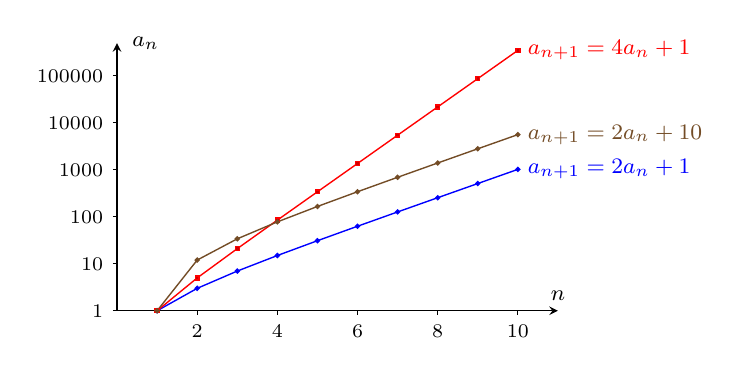
\begin{tikzpicture}
      \begin{axis}[
          scale only axis,
          width=5.6cm,
          height=3.4cm,                     % 高さを抑える(旧 4.8cm)
          clip=false,                       % 線の先の式をはみ出して表示
          % --- 軸(矢印つき・枠なし・モノクロ) ---
          axis lines=left,
          axis line style={->,>=stealth,thin,black},
          ymode=log,
          xmin=0, xmax=11,
          ymin=1, ymax=500000,
          xtick={2,4,6,8,10},
          ytick={1,10,100,1000,10000,100000},
          yticklabels={1,10,100,1000,10000,100000},
          tick align=outside,
          major tick length=1.5pt,
          minor tick length=0pt,
          tick style={black,thin},
          tick label style={font=\scriptsize,black},
          % --- 線・点(すべて黒、細く小さく) ---
          every axis plot/.append style={
            black, line width=0.5pt,
            mark=*, mark size=0.7pt, mark options={solid,fill=black},
          },
        ]
        % 軸ラベル
        \node[above]     at (rel axis cs:1,0) {\footnotesize $n$};
        \node[right=2pt] at (rel axis cs:0,1) {\footnotesize $a_n$};
   
        % p=2, q=1
        \addplot coordinates {
          (1,1) (2,3) (3,7) (4,15) (5,31)
          (6,63) (7,127) (8,255) (9,511) (10,1023)
        } node[pos=1,right,font=\footnotesize] {$a_{n+1}=2a_n+1$};
   
        % p=4, q=1
        \addplot coordinates {
          (1,1) (2,5) (3,21) (4,85) (5,341)
          (6,1365) (7,5461) (8,21845) (9,87381) (10,349525)
        } node[pos=1,right,font=\footnotesize] {$a_{n+1}=4a_n+1$};
   
        % p=2, q=10
        \addplot coordinates {
          (1,1) (2,12) (3,34) (4,78) (5,166)
          (6,342) (7,694) (8,1398) (9,2806) (10,5622)
        } node[pos=1,right,font=\footnotesize] {$a_{n+1}=2a_n+10$};
      \end{axis}
    \end{tikzpicture}
    \caption{$p,q$の値による漸化式が成す値の変化}
  \end{figure}
  
  となる.
  これが対数グラフであることに注意して観察してみると,$p$の値が数列の成す値に関して支配的であることが分かる.
  また,$q$はそこまでグラフの値の変化に大きく影響するわけでないことも分かる.
  実際,$a_n$に対して$p$が掛けられることで$a_{n+1}$が作られるのだから,等比型の一般項のように,$p^n$のような形が一般項に含まれることは比較的想像しやすいだろう.

  等比型漸化式$a_{n+1}=ra_n$の一般項が$a_n=a_1r^{n-1}$であることを思い出すと,一般項に$p^n$が含まれることが想像できる.
  そこで,$q$や$a_1$分の補正を与えてやれば漸化式から一般項を得られると考え,その方法を検討しよう.
  
  $p$に関しておおよその推測がたった今,いかにして$q$を処理するかが争点になってくる.
  今,読者諸君らが持つ技は,等比型,等差型,階差型,階比型の漸化式を解くことといくつかの基本的な計算テクニックであろう.
  基本的な計算テクニックの内,邪魔なもの,つまりは$q$を消すためにはどのような手法があるだろうか.
  邪魔な項を消す場合は以下のような方法がよく用いられる.
  \begin{enumrate}
    \item 同じ値を引く
    \item 別の等式を用意して代入\footnote{\sectionref{節：総和型}ではこの発想が用いられている}
    \item 約分できるような数で割る\footnote{\sectionref{節：分数型}ではある意味でこの亜種のような計算をする}
    \item 平方完成や部分分数分解のようなテクニックでうまく消えるような項を作る
  \end{enumrate}
  平方完成や部分分数分解ができるような複雑な見た目をしていないし,約分しようにも$q$を消す約分をしたところで,問題の本質はそこまで変わらないだろう.\footnote{$\frac{a_{n+1}}{q}=\frac{p}{q}a_{n}+1$となるが,$a_n$が定数倍されたものに定数を足したものが次の項という構造に変化はない.}
  したがって,「同じ値を引く」「別の等式を用意して代入」の2つを試してみよう.
  
  ここからがやっと解法である.
  メジャーな解法は「同じ値を引く」の方なので,先にその方法で示してから,後に「別の等式を用意して代入」の方をお見せしよう.

  \noidnent \textbf{【同じ値を引く】}
  
  結論から述べよう.
  $q$がなくなるように式変形をしてやればよいのだから
  \[
    \begin{array}{rrl}
      &a_{n+1}={}&pa_n+q\\
      -\,)&\alpha={}&p\alpha+q\\ \hline
      &a_{n+1}-\alpha={}&p(a_n-\alpha)
    \end{array}
  \]
  となるような$\alpha$を考えればよいのだ.
  
  言い換えればある実数$\alpha$によって,
  \begin{aligin*}
    a_{n+1}=pa_n+q \iff a_{n+1}-\alpha=p(a_n-\alpha)
  \end{aligin*}
  となるような$\alpha$が存在しさえしてくれれば,漸化式は等比型に帰着する.
  $\alpha$を求めると
  \begin{aigin*}
    &\alpha=p\alpha+q\\
    &\therefore \quad \alpha=\frac{q}{1-p}
  \end{aligin*}
  その後の計算は$b_n=a_n-\alpha$と置くことでもとの漸化式は公比$p$,初項$a_1-\alpha$の等比型漸化式に帰着する.
  \begin{aligin*}
    &b_{n+1}=pb_n\\
    &\therefore \quad b_n=b_1p^{n-1}\\
    &\therefore \quad a_n=(a_1-\alpha)p^{n-1}+\alpha
    &\therefore \quad a_n=(a_1-\frac{q}{1-p})p^{n-1}+\frac{q}{1-p}
  \end{aligin*}
  以上より一般項を得る.
  
  この式変形の図形的意味を考えてみよう.
  少々突飛な発想だが,
  \[
    a_{n+1}=pa_n+q
  \]
  の式を
  \[
    y=px+q
  \]
  として考えてみよう.
  つまり,$a_n$の値による$a_{n+1}$の値の変化をグラフに落とし込むということだ.
  図示すると
  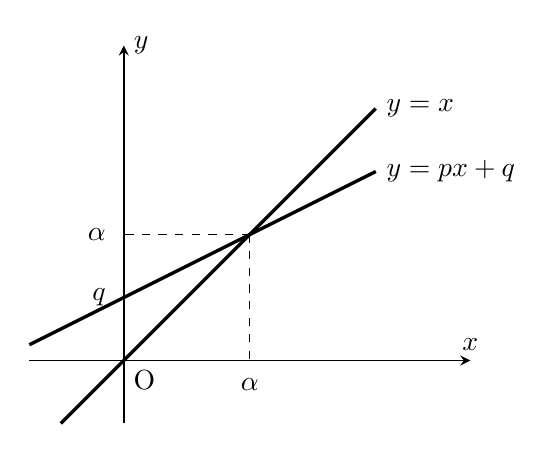
\begin{tikzpicture}[scale=0.8]
    \draw[->,>=stealth,semithick] (-1.5,0)--(5.5,0)node[above]{$x$};
    \draw[->,>=stealth,semithick] (0,-1)--(0,5)node[right]{$y$};
    \draw (0,0)node[below right]{O};
  
    \draw[very thick,domain=-1:4]
    plot(\x,\x)node[right]{$y=x$};
  
    \draw[very thick,domain=-1.5:4]
    plot(\x,\x/2+1) node[right] {$y=px+q$};
  
    % q
    \node[left=3pt] at (0,1) {$q$};
  
    % 交点から各軸へ点線
    \draw[dashed] (2,2) -- (2,0);
    \draw[dashed] (2,2) -- (0,2);
  
    % α
    \node[below=3pt] at (2,0) {$\alpha$};
    \node[left=3pt] at (0,2) {$\alpha$};
  \end{tikzpicture}
  \begin{center}
    \BookFigureCaption{直線の交点として捉える\bookterm{fixed}{不動点}}
  \end{center}

  となる.
  $y=x$のグラフは$a_{n+1}=a_n$という公比1の等比数列としてみなしたときに,これらのグラフの交点を原点と思って漸化式を見直してやれば,点$(\alpha,\alpha)$が原点であるような等比数列となるのだ.

  このような点$(\alpha,\alpha)$を不動点という.
  特性方程式は不動点を求める漸化式で,不動点は特性方程式型漸化式を等比型漸化式としてみなせるようになる(ずらすことで"きれい"にできる)点である.
  
  初項が$\alpha$なら定数解,異なるなら$|p|>1$でずれが増大し,$|p|<1$で$0$へ近づく.
  後者では$a_n\to\alpha$となる.

  \noidnent \textbf{【別の等式を用意して代入】}
  
  同じ$q$を消すには,隣り合う二つの漸化式をを引く方法もある.
  \begin{align*}
    &a_{n+1}=pa_n+q \booktag{affine-difference-1}{♡}\\
    &a_{n+2}=pa_{n+1}+q \booktag{affine-difference-2}{♢}\\
  \end{align*}
  $\bookeqbackref{affine-difference-2}{(♢)}-\bookeqbackref{affine-difference-1}{(♡)}$をし
  \[
    a_{n+2}-a_{n+1}=p(a_{n+1}-a_n)
  \]
  ここで,$d_n=a_{n+1}-a_n$と置くと,
  \[
    d_{n+1}=pd_n,\qquad d_1=(p-1)a_1+q
  \]
  となる.等比型になった\textbf{階差}$d_n=d_1p^{n-1}$を,\sectionref*{節：階差型}と同じように足し戻す.
  \begin{align*}
    a_n&=a_1+\sum_{k=1}^{n-1}d_k\\
    &=a_1+d_1\frac{p^{n-1}-1}{p-1}\\
    &=\alpha+(a_1-\alpha)p^{n-1}
  \end{align*}
  $d_1=(p-1)(a_1-\alpha)$より,不動点を引く方法と一致する.
  $p=1$の場合も階差は一定なので,$a_n=a_1+(n-1)q$と足し戻せる.
  
  二つの直線$y=px$と$y=px+q$の差は$q$である.一方,更新式どうしの引き算では異なる入力を比べる.
  $f(x)=px+q$なら,
  \[
    f(x)-f(y)=(px+q)-(py+q)=p(x-y)
  \]
  となる.$x=a_{n+1},\ y=a_n$としたものが\bookeqref{affine-difference-2}{(2)}から\bookeqref{affine-difference-1}{(1)}を引いた式である.\footnote{添字を一つずらして引く操作は,付録\sectionref{節：和と差から微積分へ}で扱う\bookterm{difference-operator}{差分}の考え方につながる.}
  共通の$q$が消えた.二つの直線も確認しよう.
  
  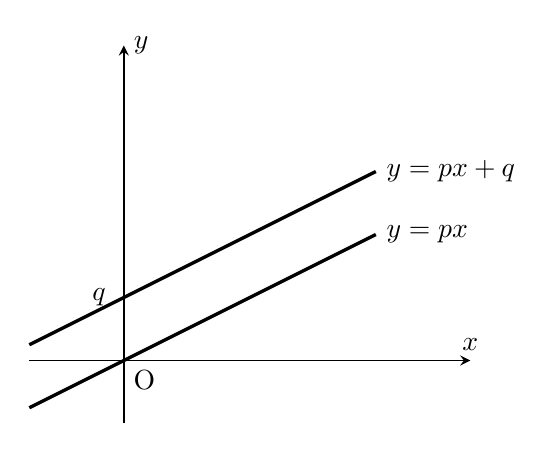
\begin{tikzpicture}[scale=0.8]
    \draw[->,>=stealth,semithick] (-1.5,0)--(5.5,0)node[above]{$x$};
    \draw[->,>=stealth,semithick] (0,-1)--(0,5)node[right]{$y$};
    \draw (0,0)node[below right]{O};
  
    \draw[very thick,domain=-1.5:4]
    plot(\x,\x/2)node[right]{$y=px$};
  
    \draw[very thick,domain=-1.5:4]
    plot(\x,\x/2+1) node[right] {$y=px+q$};
  
    % q
    \node[left=3pt] at (0,1) {$q$};
  
  \end{tikzpicture}
  \begin{center}
    \BookFigureCaption{定数項の違いを表す平行な直線}
  \end{center}
  
  不動点からのずれと隣り合う項の差は,同じ定数項を消す二つの見方である.
  この先では引く量が一次式などへ広がり,二項をまとめる際には倍率を求める\mbox{\bookterm{characteristic}{特性方程式}}が現れる.
  今の$\alpha$は変わらない値,後の根は更新の倍率である.付録の\bookterm{matrix}{行列}でもつながりを見直す.

  \noident \textbf{【$p$へのアプローチ】}
  
  ここまで$q$を消す試みを続けてきたが,$p$にたいしてうまく操作できないだろうか.
  \sectionref{節：階差階比複合型}でも使われる式変形を用いればうまく解くことができる.
  \[
    a_{n+1}=pa_n+q
  \]
  について,$p^{n+1}$で割って,
  \[
    \frac{a_{n+1}}{p^{n+1}}=\frac{a_n}{p^n}+\frac{q}{p^{n+1}}
  \]
  ここで$\displaystyle b_n=\frac{a_n}{p^n}$と置くと
  \[
    b_{n+1}=b_n+\frac{q}{p^{n+1}}
  \]
  となって階差型となる.

% subsection: 階差等比複合型 \, $\displaystyle a_{n+1}=pa_n+f(n)$

\subsection{\texorpdfstring{階差等比複合型  $\displaystyle a_{n+1}=pa_n+f(n)$}{階差等比複合型}}\label{節：階差等比複合型}
\begin{bookpoint}
  \textbf{共通の付加項を消す}\par
  同じ更新をする多項式を引くと,付加項が消える.指数の付加項には,その指数で割る方法も使える.
\end{bookpoint}
\subsubsection{\texorpdfstring{多項式を引く  $\displaystyle a_{n+1}=pa_n+f(n)$}{多項式を引く}}
\sectionref*{節：特性方程式型}では,同じ更新をする定数を引いた.
今回は付加項$f(n)$が$n$によって変わるため,引く量も$n$によって変えてみる.
\sectionref*{節：補助数列を作る}と同じく,同じ更新をする量を探す.
$f(n)$を多項式とし,$p\ne1$を考えよう.$p=1$なら\bookterm{difference}{階差}型である.

\bookstep{引く量を選ぶ}
$b_n=a_n-g(n)$を等比型にするための条件は
\[
  g(n+1)=pg(n)+f(n)
\]
である.この条件なら,
\[
  \begin{array}{rrl}
    &a_{n+1}={}&pa_n+f(n)\\
    -\,)&g(n+1)={}&pg(n)+f(n)\\ \hline
    &a_{n+1}-g(n+1)={}&p\{a_n-g(n)\}
  \end{array}
\]
となり,付加項が消える.
$a_n=g(n)+b_n$は,\sectionref*{節：解の差を取る}の「既知の解と\bookterm{homogeneous}{同次}の解」の分解である.
$g(n)$を探し,$b_n$を\bookterm{initial}{初期条件}から決める.

まず$a_{n+1}=2a_n+n-1$で試してみよう.
付加項が一次式なので,引く量も$g(n)=un+v$と置く.
一次式は添字を一つずらしても一次式のままである.
元の付加項と次数をそろえ,未知の係数$u,v$で残る項を消そう.
条件$g(n+1)=2g(n)+n-1$に代入すると,
\[
  un+u+v=(2u+1)n+2v-1
\]
となる.すべての$n\ge1$で成り立つよう係数を合わせると,
\[
  u=2u+1,\qquad u+v=2v-1
\]
より$u=-1,\ v=0$,すなわち$g(n)=-n$を得る.
従って
\[
  a_{n+1}+(n+1)=2(a_n+n)
\]
となる.初項$a_1+1$から,
\[
  a_n=(a_1+1)2^{n-1}-n
\]
と元へ戻せる.この例は\bookproblemref{practice-basic}{4}{標準問4}でも扱う.

\bookstep{多項式へ広げる}
同じ手順を,$f(n)$が$m$次式の場合に広げよう.
$p\ne1$のときは$m$次の多項式
\[
  g(n)=x_0+x_1n+\cdots+x_mn^m
\]
を候補にする.$g(n+1)-pg(n)$の最高次の係数は$(1-p)x_m$である.
これを$f(n)$の最高次の係数に合わせ,次に一段低い係数を合わせる.
$1-p\ne0$なので,この順に$x_m,x_{m-1},\ldots,x_0$を決められる.\footnote{未知の係数を比較して求めるこの方法を\bookterm{undetermined}{未定係数法}という.}

\bookstep{変形と復元}
$b_{n+1}=pb_n$を解き,$a_n=b_n+g(n)$へ戻す.
$p\ne0,1$なら
\[
  a_n=\{a_1-g(1)\}p^{n-1}+g(n)
\]
となる.\footnote{$p=0$なら初項を別に扱い,$n\ge2$で$a_n=f(n-1)$と直接求める.}
一方,$p=1$で$f(n)$が$m$次なら,付加項を足し戻す多項式は通常$m+1$次になる.
例えば$a_{n+1}=a_n+n$では,$g(n)=\frac{n(n-1)}2$が同じ更新を満たす.

\subsubsection{\texorpdfstring{指数で割る   $\displaystyle a_{n+1}=pa_n+q^n$}{指数で割る}}
$a_{n+1}=pa_n+q^n$では,指数で割ると付加項が定数になる.$q\ne0$とする.\footnote{$q=0$なら$n\ge1$で$q^n=0$なので等比型になる.}
付加項$q^n$を$1$にするために,両辺を$q^n$で割る.
左辺の添字は$n+1$なので,それに合わせて第$n$項を割る量は$q^{n-1}$とする.
両辺を$q^n$で割り,$b_n=\dfrac{a_n}{q^{n-1}}$と置くと,
\[
  \begin{aligned}
    \frac{a_{n+1}}{q^n}&=\frac pq\frac{a_n}{q^{n-1}}+1,\\
    b_{n+1}&=\frac pq b_n+1.
  \end{aligned}
\]
\booknavref{節：特性方程式型}{特性方程式型}へ戻った.
ただし$p=q$のときは$b_{n+1}=b_n+1$(\bookterm{arithmetic}{等差数列})になり,\bookterm{fixed}{不動点}$\alpha$が存在しない.\footnote{\bookproblemref{example-characteristic-1}{3}{先ほどの例題(3)}と同じ状況である.}
この場合は$b_n=b_1+(n-1)$として直接求まる.
いずれの場合も,求めた$b_n$に$q^{n-1}$を掛ければ元の$a_n$に戻る.
例えば$a_1=1,\,a_{n+1}=2a_n+2^n$($p=q=2$)ならば$b_n=\dfrac{a_n}{2^{n-1}}$が\bookterm{arithmetic}{等差数列}となり,$a_n=n\cdot2^{n-1}$が得られる.

% subsection: 対数型 \, $a_{n+1}=pa_n^q$

\subsection{\texorpdfstring{対数型  $a_{n+1}=pa_n^q$}{対数型}}\label{節：対数型}
  今までは$a_n$に対して$f(n)$を足したり掛けたりしてきたが,$a_n$自体を掛けたり足したりしたらどうなるだろう.

  まずはシンプルに
  \[
    a_{n+1}=pa_n^q
  \]
  という漸化式を考えてみることにする.
  さて,いかにして既知の形に帰着させようか.
  $n$倍であったり,$n$を足すことに関してはここまでの内容を押さえた読者ならばできることだろう.
  しかし$n$乗をするという操作については今までしたことがない.
  この$n$乗という操作を足したり掛けたりすることにできれば解くことができそうだ.
  ここで1つの知識を思い出そう.
  対数は積を指数の足し算や掛け算としてあつかうことができるようにするものだった.
  だから,今回のように積を和の形に変換するのにはうってつけの道具であろう.\footnote{ \sectionref*{節：指数と対数}で対数について扱っている.対数に自身がない人は参照すると良い.}

  ここで1つ断りをいれておこう.
  対数の真数条件から,この節で扱う$a_n$はすべて0より大きい実数であるとする.
  以後断りなしに対数をとるが,答案等に書く際は常に真数条件を確かめる.\footnote{$a_n>0$ならば$p a_n^q>0$であるから,\bookterm{induction}{数学的帰納法}によりすべての項が正となり,\bookterm{logarithm}{対数}を取ることができる.}こと.
  

  実際に両辺の対数を取ってみると,
  \begin{align*}
      \log_pa_{n+1}&=\log_pp+q\log_pa_n\\
      &=q\log_pa_n+1.
  \end{align*}
  ここで底を$p$とする対数をとったが,底は何を選んでもよい.しかし,後の計算のためになるべく$p$や$r$などの数を底としておくとよい.
  $b_n=\log_pa_n$とおくと
  \[
    b_{n+1}=qb_n+1
  \]
  を得る.
  よってこの漸化式は特性方程式漸化式になったので,これを解くと
  \[
    b_n=\left(a_1-\frac{1}{1-q}\right)q^{n-1}+\frac{1}{1-q}
  \]\
  となる.\footnote{$q=1$のときはそもそも特性方程式漸化式ではなく,等差型漸化式に帰着させて解く}
  したがって
  \[
    b_n=\log_p a_n  \iff a_n=p^{b_n}
  \]
  であることから,一般項を得る.
  
  \noindent\bookblocklink{example-logarithmic-1}{problem}{answer}{【例題】}\par\nobreak
  \begin{enumerate}[label=(\arabic*),parsep=3pt,format=\bookitemlink{example-logarithmic-1}{problem}{answer}]
    \item $\displaystyle a_1=2,\quad a_{n+1}=2a_n^2$
    \item $\displaystyle a_1=\frac{1}{2},\quad a_{n+1}=\frac{1}{a_n}$
    \item $\displaystyle a_1=1,\quad a_{n+1}=2^na_n$
    \item $\displaystyle a_1=5,\quad a_{n+1}=a_n^2-2a_n+2$
    \item $\displaystyle a_1=2,\quad a_{n+1}=\frac{a_n^2}{2^n}$
    \item $\displaystyle a_1=1,\quad a_{n+1}=(n+1)a_n$
  \end{enumerate}
  
  \noindent\bookblocklink{example-logarithmic-1}{hint}{problem}{【方針】}\par\nobreak
  \begin{enumerate}[label=(\arabic*),parsep=3pt,format=\bookitemlink{example-logarithmic-1}{hint}{problem}]
    \item $b_n=\log_2a_n$で$b_{n+1}=2b_n+1$に変え,定数項を消します.
    \item 逆数を\bookterm{logarithm}{対数}で符号反転に変えます.
    \item $f(n)=2^n$が指数関数なので,\bookterm{logarithm}{対数}を取ると和の形に帰着できます.
    \item \bookterm{square}{平方完成}で$a_{n+1}-1=(a_n-1)^2$を作ります.\bookterm{logarithm}{対数}を取る量は$a_n$ではなく$a_n-1$であり,その正値を先に確認します.
    \item $b_n=\log_2a_n$から一次式$n+1$を引くと等比型になります.
    \item 積を直接まとめる方法と,\bookterm{logarithm}{対数}で和に変える方法を比べましょう.最後には同じ積$n!$を計算します.
  \end{enumerate}
  
  \noindent\bookblocklink{example-logarithmic-1}{answer}{problem}{【解答】}\par\nobreak
  \begin{enumerate}[label=(\arabic*),parsep=3pt,format=\bookitemlink{example-logarithmic-1}{answer}{problem}]
    \item $\displaystyle a_n=2^{2^{n}-1}$
    \item $a_n=2^{(-1)^{n}}$
    \item $a_n=2^{\frac{n(n-1)}{2}}$
    \item $a_n=2^{2^n}+1$
    \item $\displaystyle a_n=2^{\,n+1-2^{n-1}}$
    \item $a_n=n!$
  \end{enumerate}
  
  \noindent\bookblocklink{example-logarithmic-1}{solution}{problem}{【解法】}\par\nobreak
  
  (1),(2),(3),(5),(6)は初項が正で,正の項から次も正になる.\bookterm{induction}{数学的帰納法}より全項が正である.
  (4)は$a_1-1=4>0$と$a_{n+1}-1=(a_n-1)^2$から,$a_n-1>0$を保つ.この量に\bookterm{logarithm}{対数}を取る.
  \begin{enumerate}[label=(\arabic*),parsep=3pt,format=\bookitemlink{example-logarithmic-1}{solution}{problem}]
    \item $b_n=\log_2a_n$と置くと,
      \[
        b_{n+1}=2b_n+1,\qquad b_1=1.
      \]
      $b_n+1$は初項$2$,公比$2$の等比型なので,
      \[
        b_n+1=2^n,\qquad a_n=2^{b_n}=2^{2^n-1}.
      \]
    \item $b_n=\log_2a_n$と置くと,逆数は
      \[
        b_{n+1}=-b_n,\qquad b_1=\log_2\frac12=-1
      \]
      に変わる.従って$b_n=(-1)^n$であり,$a_n=2^{(-1)^n}$となる.
    \item 自然\bookterm{logarithm}{対数}を取れば$\log a_{n+1}=\log a_n+n\log2$である.差を足すと,
      \[
        \log a_n=\sum_{k=1}^{n-1}k\log2=\frac{n(n-1)}2\log2.
      \]
      従って$a_n=2^{\dfrac{n(n-1)}{2}}$となる.
    \item \bookterm{square}{平方完成}で$a_{n+1}-1=(a_n-1)^2$となる.\bookterm{logarithm}{対数}を取ると,
      \[
        \log_2(a_{n+1}-1)=2\log_2(a_n-1).
      \]
      初項は$\log_2(a_1-1)=2$だから,$\log_2(a_n-1)=2^n$であり,$a_n=2^{2^n}+1$となる.
    \item $b_n=\log_2a_n$と置くと,$b_{n+1}=2b_n-n,\ b_1=1$である.
      一次式$n+1$を引けば,
      \[
        b_{n+1}-(n+2)=2\{b_n-(n+1)\}.
      \]
      $c_n=b_n-(n+1)$は$c_{n+1}=2c_n,\ c_1=-1$を満たすので,
      \[
        c_n=-2^{n-1},\quad b_n=n+1-2^{n-1}.
      \]
      戻すと$a_n=2^{\,n+1-2^{n-1}}$となる.
    \item 自然\bookterm{logarithm}{対数}を取れば$\log a_{n+1}=\log a_n+\log(n+1)$である.
      \[
        \log a_n=\log1+\log2+\cdots+\log n=\log n!.
      \]
      従って$a_n=n!$となる.直接積を取っても同じ結果が得られる.
  \end{enumerate}
  \noindent\textbf{【補足】}
  
  (3),(6)の$\log$は底が$e$の自然\bookterm{logarithm}{対数}である.
  変形後の真数が$0$や負なら,実数の\bookterm{logarithm}{対数}は取れない.例えば(4)で初項が$1$なら定数\bookterm{sequence}{数列}$a_n=1$となり,$\log(a_n-1)$を取らずに扱う.
  
  \noindent\bookblocklink{check-log-domain}{problem}{answer}{【確認問題】}\par\nobreak
  \begin{enumerate}[format=\bookitemlink{check-log-domain}{problem}{answer}]
    \item $a_{n+1}=a_n^2$で,初項が$2,0,-2$の場合を比較せよ.
      最初から実数の\bookterm{logarithm}{対数}を取れるのはどの場合か.取れない場合にも\bookterm{sequence}{数列}は定義されるか.
  \end{enumerate}
  \noindent\bookblocklink{check-log-domain}{answer}{problem}{【確認の解答】}\par\nobreak
  \begin{enumerate}[format=\bookitemlink{check-log-domain}{answer}{problem}]
    \item 初項$2$ならすべての項が正である.
      初項$0$なら零列,初項$-2$なら第2項以降が正である.
      いずれも元の\bookterm{recurrence}{漸化式}は定義される.\bookterm{logarithm}{対数}を取る条件と,元の\bookterm{sequence}{数列}が存在する条件は区別する.
  \end{enumerate}

% parent file: 分数型
\subsection{分数型}\label{節：分数型}
\begin{bookpoint}
  \textbf{分母を簡単にする}\par
  逆数,または\bookterm{fixed}{不動点}からの二つの差の比を追う.
  分母が零になる初期値と定数解の分岐を確かめてから,置き換えを使う.
\end{bookpoint}
% subsubsection: 逆数型  \, $\displaystyle a_{n+1}=\frac{pa_n}{qa_n+r}$

\subsubsection{\texorpdfstring{逆数型   $\displaystyle a_{n+1}=\frac{pa_n}{qa_n+r}$}{逆数型}}\label{節：逆数型}
分子が$a_n$の定数倍である\bookterm{recurrence}{漸化式}を考えよう.
逆数を取れば,分母にあった一次式を$a_n$で割り,定数と$\frac1{a_n}$の和に分けられる.
以下では,$p\ne0$かつ$a_n\ne0$であり,$qa_n+r\ne0$として議論する.\footnote{$a_1=0$は逆数を取る前に分ける.$r\ne0$ならすべての項が$0$となる.$r=0$なら最初の更新から分母が$0$となり,そのままでは定義できない.}
両辺の逆数を取り,$b_n=\dfrac{1}{a_n}$と置くと,
\begin{align*}
  \frac{1}{a_{n+1}}&=\frac{qa_n+r}{pa_n}
  =\frac{q}{p}+\frac{r}{p}\cdot\frac{1}{a_n},\\
  b_{n+1}&=\frac{r}{p}b_n+\frac{q}{p}
\end{align*}
ここから特性方程式型または等差型として$b_n$を求め,最後に$a_n=\dfrac{1}{b_n}$へ戻す.
ただし$b_n=0$となる項は逆数を戻せないため,元の漸化式が定義されるかも確認する.

\noindent \bookblocklink{example-reciprocal-1}{problem}{answer}{【例題】}\par\nobreak
\begin{enumerate}[label=(\arabic*),parsep=3pt,format=\bookitemlink{example-reciprocal-1}{problem}{answer}]
  \item $\displaystyle a_1=1,\, a_{n+1}=\frac{a_n}{a_n+1}$
  \item $\displaystyle a_1=1,\, a_{n+1}=\frac{-a_n}{2a_n+1}$
\end{enumerate}

\noindent\bookblocklink{example-reciprocal-1}{hint}{problem}{【方針】}\par\nobreak
\begin{enumerate}[label=(\arabic*),parsep=3pt,format=\bookitemlink{example-reciprocal-1}{hint}{problem}]
  \item 逆数を取ると,$\dfrac{1}{a_n}$が毎回$1$ずつ増える形になります.
  \item 逆数を取って一次の\bookterm{recurrence}{漸化式}に帰着させましょう.
\end{enumerate}

\noindent\bookblocklink{example-reciprocal-1}{answer}{problem}{【解答】}\par\nobreak
\begin{enumerate}[label=(\arabic*),parsep=3pt,format=\bookitemlink{example-reciprocal-1}{answer}{problem}]
  \item $\displaystyle a_n=\frac{1}{n}$
  \item $\displaystyle a_n=\frac{1}{2(-1)^{n-1}-1}$
\end{enumerate}

\noindent\bookblocklink{example-reciprocal-1}{solution}{problem}{【解法】}\par\nobreak
\begin{enumerate}[label=(\arabic*),parsep=3pt,format=\bookitemlink{example-reciprocal-1}{solution}{problem}]
  \item $\displaystyle a_1=1,\, a_{n+1}=\frac{a_n}{a_n+1}$\\
    正の項と分母が続くので,逆数を取れる.$b_n=\dfrac{1}{a_n}$と置くと,
    \begin{align*}
      &\frac{1}{a_{n+1}}=1+\frac{1}{a_n},\\
      &b_{n+1}=b_n+1,\quad b_1=1\\
      &\therefore \quad b_n=n,\quad a_n=\frac1n
    \end{align*}
  \item $\displaystyle a_1=1,\, a_{n+1}=\frac{-a_n}{2a_n+1}$\\
    初めの更新は$1\longmapsto-\dfrac{1}{3}\longmapsto1$となる.
    項も分母も零でないので,$b_n=\dfrac{1}{a_n}$と置くと,
    \begin{align*}
      &\frac{1}{a_{n+1}}=-2-\frac{1}{a_n},\\
      &b_{n+1}=-b_n-2,\quad b_1=1
    \end{align*}
    \bookterm{fixed}{不動点}は$-1$なので,$c_n=b_n+1$と置き,定数項を消す.
    \begin{align*}
      &c_{n+1}=-c_n,\quad c_1=2\\
      &\therefore \quad b_n=c_n-1=2(-1)^{n-1}-1,\\
      &a_n=\frac{1}{2(-1)^{n-1}-1}
    \end{align*}
\end{enumerate}

% subsubsection: 1次分数型  \, $\displaystyle a_{n+1}=\frac{pa_n+q}{ra_n+s}$

\subsubsection{\texorpdfstring{一次分数型   $\displaystyle a_{n+1}=\frac{pa_n+q}{ra_n+s}$}{一次分数型}}\label{節：一次分数型}
分子にも定数項がある\bookterm{recurrence}{漸化式}を考えよう.
以下では$r\ne0$, $ps-qr\ne0$とし,元の分母が$0$にならない範囲で議論する.\footnote{$r=0,\ s\ne0$なら特性方程式型へ戻る.
  $r\ne0,\ ps-qr=0$なら,分母が非零の入力に対して右辺は定数$\dfrac{p}{r}$になる.次の分母も確認する.例えば$\dfrac{a_n-1}{a_n-1}$は,初項が$1$でなくても次項が$1$になり,次の更新は定義できない.}
分子の定数項$q$を消せれば,逆数型として解ける.
逆数型という既知の行き先ができたので,定数を引く方法をここでも試す.
$\alpha$は変形後の分子を見て決める.

\bookstep{一つの差を追う}
\sectionref{節：特性方程式型}と同じく,各項から定数を引いてみよう.
$u_n=a_n-\alpha$と置き,分子の定数項が消えるように$\alpha$を選ぶ.
$a_n=u_n+\alpha$を代入すると,
\BookMathLayout{\begin{align*}
    u_{n+1}&=\frac{p(u_n+\alpha)+q}{r(u_n+\alpha)+s}-\alpha\\
    &=\frac{(p-r\alpha)u_n+p\alpha+q-r\alpha^2-s\alpha}
    {ru_n+r\alpha+s}
  \end{align*}}{\[
    \begin{aligned}
      &u_{n+1}\\
      &{}=\frac{p(u_n+\alpha)+q}{r(u_n+\alpha)+s}-\alpha\\
      &{}=\frac{(p-r\alpha)u_n+p\alpha+q-r\alpha^2-s\alpha}
      {ru_n+r\alpha+s}
    \end{aligned}
  \]}
従って,
\[
  r\alpha^2+(s-p)\alpha-q=0
  \quad\Longleftrightarrow\quad
  \alpha=\frac{p\alpha+q}{r\alpha+s}
\]
を満たす$\alpha$,すなわち元の\bookterm{fixed}{不動点}を引けば,
\[
  u_{n+1}=\frac{(p-r\alpha)u_n}{ru_n+r\alpha+s}
\]
という逆数型になる.ここで,$p-r\alpha$も$r\alpha+s$も零でない.\footnote{不動点の方程式より,$(p-r\alpha)(r\alpha+s)=ps-qr\ne0$.}
初項が$\alpha$なら定数列である.それ以外では$u_n$は途中で零にならず,逆数を取って解ける.

\bookstep{二つの差の比を追う}
不動点の方程式
\[
  rx^2+(s-p)x-q=0
\]
が異なる二つの実数解$\alpha,\beta$を持つとしよう.
どちらも定数項を消せるので,先ほどの変形を$a_n$で書けば,
\begin{align*}
  a_{n+1}-\alpha
  &=\frac{p-r\alpha}{ra_n+s}(a_n-\alpha),\\
  a_{n+1}-\beta
  &=\frac{p-r\beta}{ra_n+s}(a_n-\beta)
\end{align*}
となる.倍率に$a_n$が含まれるため,各々の差は一般には\bookterm{geometric}{等比数列}にならない.
しかし,\textbf{二つの式の比を取れば,共通の分母が消える}.
一つの差を作っても残った分母を,もう一つの差と組み合わせて取り除くのである.

初項が$\alpha$または$\beta$なら定数\bookterm{sequence}{数列}として分けておく.
それ以外では,$p-r\beta\ne0$なので,$a_n\ne\beta$から$a_{n+1}\ne\beta$が続く.
従って,差の比を取れる.
\begin{align*}
  \frac{a_{n+1}-\alpha}{a_{n+1}-\beta}
  &=\frac{p-r\alpha}{p-r\beta}
  \frac{a_n-\alpha}{a_n-\beta}
\end{align*}
ここで$b_n=\dfrac{a_n-\alpha}{a_n-\beta}$と置けば,
\[
  b_{n+1}=\frac{p-r\alpha}{p-r\beta}b_n
\]
となる.一つの差を逆数型として解く代わりに,二つの差の比を直接等比型にできた.\footnote{二つの解のどちらを$\alpha,\beta$と名付けてもよい.}
初項$b_1=\dfrac{a_1-\alpha}{a_1-\beta}$を用いて,
\[
  b_n=\frac{a_1-\alpha}{a_1-\beta}\left(\frac{p-r\alpha}{p-r\beta}\right)^{n-1} \booktag{mobius-geometric}{＊}
\]
を得る.

\bookstep{元の項へ戻す}
$b_n(a_n-\beta)=a_n-\alpha$を$a_n$について解くと,
\[
  a_n=\frac{\beta b_n-\alpha}{b_n-1}
\]
となる.有限の$a_n$では$\alpha\ne\beta$より$b_n\ne1$なので,この割り算ができる.
\bookeqbackref{mobius-geometric}{(＊)}を代入すればよい.
逆に,公式上で$b_n=1$となる項は復元できず,元の更新をそこまで定義できない.

不動点の方程式が重解$\alpha$を持つ場合は,異なる差を作れない.
一つの差$u_n=a_n-\alpha$に戻り,逆数を取れば等差型になる.
例題(3)で計算し,例題の後で一般の係数でも確かめよう.

\noindent \bookblocklink{example-mobius-1}{problem}{answer}{【例題】}\par\nobreak
\begin{enumerate}[label=(\arabic*),parsep=3pt,format=\bookitemlink{example-mobius-1}{problem}{answer}]
  \item $\displaystyle a_1=3,\, a_{n+1}=\frac{2a_n+1}{a_n+2}$
  \item $\displaystyle a_1=0,\, a_{n+1}=\frac{a_n+4}{a_n+1}$
  \item $\displaystyle a_1=5,\, a_{n+1}=\dfrac{4a_{n}-9}{a_{n}-2}$
  \item $\displaystyle a_1=1,\, a_{n+1}=1+\frac{1}{a_n}$
\end{enumerate}

\noindent\bookblocklink{example-mobius-1}{hint}{problem}{【方針】}\par\nobreak
\begin{enumerate}[label=(\arabic*),parsep=3pt,format=\bookitemlink{example-mobius-1}{hint}{problem}]
  \item 不動点$1,-1$からの差の比を作ると,共通の分母$a_n+2$が消えます.
  \item 同様に\bookterm{fixed}{不動点}$\alpha,\beta$を求めましょう.今回は片方が負の値になります.
  \item 今回は\bookterm{fixed}{不動点}の方程式が重解になります.$\dfrac{a_n-\alpha}{a_n-\beta}$は使えないので,$b_n=a_n-\alpha$と置いてから逆数型に帰着させる別の手法を使います.
  \item このような形も一次分数型です.解と係数の関係を活用して解きましょう.
\end{enumerate}

\noindent\bookblocklink{example-mobius-1}{answer}{problem}{【解答】}\par\nobreak
\begin{enumerate}[label=(\arabic*),parsep=3pt,format=\bookitemlink{example-mobius-1}{answer}{problem}]
  \item $\displaystyle a_n=\frac{2\cdot3^{n-1}+1}{2\cdot3^{n-1}-1}$
  \item $\displaystyle a_n=\frac{2\left(3^{n-1}+(-1)^n\right)}{3^{n-1}-(-1)^n}$
  \item $a_{n}=\dfrac{6n-1}{2n-1}$
  \item $\displaystyle a_n=\cfrac{\left(\cfrac{1-\sqrt{5}}{2}\right)^{n+1}-\left(\cfrac{1+\sqrt{5}}{2}\right)^{n+1}}{\left(\cfrac{1-\sqrt{5}}{2}\right)^n-\left(\cfrac{1+\sqrt{5}}{2}\right)^n}$
\end{enumerate}

\noindent\bookblocklink{example-mobius-1}{solution}{problem}{【解法】}\par\nobreak
\begin{enumerate}[label=(\arabic*),parsep=3pt,format=\bookitemlink{example-mobius-1}{solution}{problem}]
  \item $\displaystyle a_1=3,\, a_{n+1}=\frac{2a_n+1}{a_n+2}$\\
    \bookterm{fixed}{不動点}の方程式$x=\dfrac{2x+1}{x+2}$の解は$1,-1$である.
    $b_n=\dfrac{a_n-1}{a_n+1}$と置くと,
    \begin{align*}
      b_{n+1}&=\cfrac{\cfrac{2a_n+1}{a_n+2}-1}{\cfrac{2a_n+1}{a_n+2}+1}\\
      &=\frac{2a_n+1-(a_n+2)}{2a_n+1+(a_n+2)}\\
      &=\frac13\frac{a_n-1}{a_n+1}=\frac13b_n
    \end{align*}
    $b_1=\dfrac{3-1}{3+1}=\dfrac{1}{2}$なので,
    \[
      b_n=\frac12\left(\frac13\right)^{n-1}
      =\frac1{2\cdot3^{n-1}}
    \]
    である.元の項への復元は,
    \begin{align*}
      b_n(a_n+1)&=a_n-1,\\
      a_n&=\frac{1+b_n}{1-b_n}
      =\frac{2\cdot3^{n-1}+1}{2\cdot3^{n-1}-1}
    \end{align*}
    となる.
  \item $\displaystyle a_1=0,\, a_{n+1}=\frac{a_n+4}{a_n+1}$\\
    \bookterm{fixed}{不動点}の方程式$x=\dfrac{x+4}{x+1}$の解は$2,-2$である.
    倍率は$\dfrac{1-2}{1+2}=-\dfrac{1}{3}$なので,$b_n=\dfrac{a_n-2}{a_n+2}$と置くと,
    \begin{align*}
      b_{n+1}&=-\frac13b_n,\quad b_1=-1,\\
      b_n&=(-1)\left(-\frac13\right)^{n-1}
      =\frac{(-1)^n}{3^{n-1}}
    \end{align*}
    を得る.$b_n(a_n+2)=a_n-2$から復元して,
    \begin{align*}
      a_n&=\frac{2(1+b_n)}{1-b_n}\\
      &=\frac{2\left(3^{n-1}+(-1)^n\right)}{3^{n-1}-(-1)^n}
    \end{align*}
    となる.
  \item $\displaystyle a_1=5,\, a_{n+1}=\dfrac{4a_n-9}{a_n-2}$\\
    \bookterm{fixed}{不動点}の方程式$x=\dfrac{4x-9}{x-2}$は重解$3$を持つ.
    $b_n=a_n-3$と置くと,
    \begin{align*}
      b_{n+1}&=\frac{4a_n-9}{a_n-2}-3
      =\frac{a_n-3}{a_n-2}\\
      &=\frac{b_n}{b_n+1},\quad b_1=2
    \end{align*}
    となる.正の$b_n$が続くので,$b_n$も元の分母$b_n+1$も零でない.
    逆数を取れば,
    \begin{align*}
      \frac1{b_{n+1}}&=\frac1{b_n}+1,\\
      \frac1{b_n}&=\frac12+(n-1)=\frac{2n-1}{2}
    \end{align*}
    である.従って,
    \[
      a_n=3+b_n=3+\frac2{2n-1}=\frac{6n-1}{2n-1}
    \]
    を得る.
  \item $\displaystyle a_1=1,\, a_{n+1}=1+\frac1{a_n}$\\
    右辺を$\dfrac{a_n+1}{a_n}$と書けば,一次分数型である.
    \bookterm{fixed}{不動点}の方程式
    \[
      x=\frac{x+1}{x}\booktag{mobius-example-fixed}{1}
    \]
    の解を
    \[
      \alpha=\frac{1+\sqrt5}{2},\qquad
      \beta=\frac{1-\sqrt5}{2}
    \]
    とする.\bookeqbackref{mobius-example-fixed}{(1)}の解と係数の関係から,
    \[
      \alpha+\beta=1,\qquad \alpha\beta=-1
      \booktag{mobius-example-roots}{2}
    \]
    である.$b_n=\dfrac{a_n-\alpha}{a_n-\beta}$と置くと,
    \begin{align*}
      b_{n+1}&=\frac{a_n+1-\alpha a_n}{a_n+1-\beta a_n}\\
      &=\frac{(1-\alpha)a_n+1}{(1-\beta)a_n+1}
      \booktag{mobius-example-ratio}{3}
    \end{align*}
    となる.\bookeqbackref{mobius-example-roots}{(2)}を\bookeqbackref{mobius-example-ratio}{(3)}に使えば,
    \begin{align*}
      b_{n+1}&=\frac{\beta a_n-\alpha\beta}{\alpha a_n-\alpha\beta}\\
      &=\frac{\beta(a_n-\alpha)}{\alpha(a_n-\beta)}
      =\frac\beta\alpha b_n
    \end{align*}
    である.$b_1=\dfrac{1-\alpha}{1-\beta}=\dfrac{\beta}{\alpha}$より,
    \[
      b_n=\left(\frac\beta\alpha\right)^n
    \]
    となる.復元式$a_n=\dfrac{\beta b_n-\alpha}{b_n-1}$に代入し,分母分子に$\alpha^n$を掛けると,
    \begin{align*}
      a_n&=\frac{\beta^{n+1}-\alpha^{n+1}}{\beta^n-\alpha^n}\\
      &=\cfrac{\left(\cfrac{1-\sqrt5}{2}\right)^{n+1}-\left(\cfrac{1+\sqrt5}{2}\right)^{n+1}}
      {\left(\cfrac{1-\sqrt5}{2}\right)^n-\left(\cfrac{1+\sqrt5}{2}\right)^n}
    \end{align*}
    を得る.
\end{enumerate}
\bookstep{一つの不動点から進む}
不動点の方程式が重解$\alpha$を持つときは,差の比を作れない.
$\alpha=\dfrac{p-s}{2r}$なので,$c=p-r\alpha=r\alpha+s\ne0$と置けば,
\[
  a_{n+1}-\alpha
  =\frac{c(a_n-\alpha)}{r(a_n-\alpha)+c}
\]
となる.$a_1=\alpha$なら定数\bookterm{sequence}{数列}として分ける.
それ以外では,分母が非零の範囲で$c\ne0$より
\[
  a_{n+1}-\alpha=0
  \quad\Longleftrightarrow\quad a_n-\alpha=0
\]
であり,途中で$\alpha$に到達しない.従って逆数を取れて,
\[
  \frac1{a_{n+1}-\alpha}
  =\frac1{a_n-\alpha}+\frac rc
\]
という\bookterm{arithmetic}{等差数列}に帰着する.
\textbf{異なる不動点なら二つの差の比,重解なら一つの差の逆数}を追えばよい.
例題(3)は$\alpha=3,\ r=c=1$なので,逆数が毎回$1$ずつ増えた.

\bookstep{比から見える数列}
例題(4)は,フィボナッチ\bookterm{sequence}{数列}$F_1=F_2=1,\ F_{n+2}=F_{n+1}+F_n$とつながる.
隣接項の比$\dfrac{F_{n+1}}{F_n}$は同じ更新$a_{n+1}=1+\dfrac{1}{a_n}$と初項$1$を満たすので,$a_n=\dfrac{F_{n+1}}{F_n}$である.
この比の\bookterm{limit}{極限}は黄金比$\dfrac{1+\sqrt5}{2}$となる.\footnote{リュカ数列も同じ\bookterm{characteristic}{特性方程式}$x^2=x+1$を持ち,隣接項の比が黄金比へ収束する.
  トリボナッチ数列では$x^3=x^2+x+1$となり,比の極限は約$1.839$のトリボナッチ定数になる.}

\bookstep{項を並べて予想する}
一次分数型では,初めの数項から一般項を予想し,帰納法で確かめる方法もある.
数項を求める誘導があれば,分母と分子の増え方にも注目しよう.例題(3)で試す.\\
\noindent\bookblocklink{example-mobius-2}{problem}{answer}{【例題】}\par\nobreak
\begin{quote}
  以下の\bookterm{recurrence}{漸化式}
  \[
    a_1=5,\, a_{n+1}=\dfrac{4a_{n}-9}{a_{n}-2}
  \]
  を満たす\bookterm{sequence}{数列}$a_n$の\bookterm{general}{一般項}を帰納法を用いて求めよ.
\end{quote}
\bookblocklink{example-mobius-2}{hint}{problem}{【方針】}
\begin{quote}
  実験的に代入計算をしてみると,
  \[
    a_1=\frac{5}{1},\,a_2=\frac{11}{3},\,a_3=\frac{17}{5},\,a_4=\frac{23}{7},\,a_5=\frac{29}{9}
  \]
  となる.分母が2ずつ,分子が6ずつ増えていることから,\bookterm{general}{一般項}は
  \[
    a_n=\frac{6n-1}{2n-1}
  \]
  と予想する.
\end{quote}
\bookblocklink{example-mobius-2}{answer}{problem}{【解答】}
\begin{quote}
  予想した\bookterm{general}{一般項}を確かめる.$n=1$では$\dfrac{6-1}{2-1}=5$なので成立する.
  正の整数$k$について,
  \[
    a_k=\frac{6k-1}{2k-1}
  \]
  が成り立つと仮定する.このとき,\bookterm{recurrence}{漸化式}より,
  \begin{align*}
    a_{k+1}&=\frac{4(6k-1)-9(2k-1)}{6k-1-2(2k-1)}\\
    &=\frac{6k+5}{2k+1}
    =\frac{6(k+1)-1}{2(k+1)-1}
  \end{align*}
  分母$a_k-2=\dfrac{2k+1}{2k-1}$も零でなく,$n=k+1$で成立する.
  帰納法より,$a_n=\dfrac{6n-1}{2n-1}$がすべての正の整数$n$で成り立つ.\qed

\end{quote}

% subsubsection: 極形式による図形的解釈

\subsubsection{複素平面で見る}

前節で追った二つの差の比
\[
  b_n=\frac{a_n-\alpha}{a_n-\beta}
\]
を,\bookterm{complex-plane}{複素平面}上で考えよう.
点$a_n$から二つの\bookterm{fixed}{不動点}までの距離の比は,
\[
  \frac{|a_n-\alpha|}{|a_n-\beta|}=|b_n|
\]
である.分母のベクトル$a_n-\beta$から分子のベクトル$a_n-\alpha$へ測る有向角は,
$b_n$の\bookterm{argument}{偏角}$\arg b_n$に対応する.
つまり,次の図の\textbf{長さの比と角度の差}を,一つの複素数$b_n$で表せる.
\BookFigMobius

$b_{n+1}=\lambda b_n$なら,長さの比は$|\lambda|$倍され,角度の差は$\arg\lambda$だけ増える.
特に$|\lambda|=1$なら,$b_n$は原点からの距離を保って回転する.

係数$p,q,r,s$が実数で,不動点の方程式
\[
  rx^2+(s-p)x-q=0
\]
が非実の二解を持つ場合を考えよう.二解は\bookterm{conjugate}{共役}なので,$\beta=\overline\alpha$と選べる.
前節の変形から,
\[
  b_n=\frac{a_n-\alpha}{a_n-\overline\alpha},\qquad
  b_{n+1}=\lambda b_n,
\]
\[
  \lambda=\frac{p-r\alpha}{p-r\overline\alpha}
\]
となる.分子と分母も共役なので,$|\lambda|=1$である.
\bookterm{polar}{極形式}で
\begin{align*}
  \lambda&=\cos\theta+i\sin\theta,\\
  b_n&=\rho_n(\cos\varphi_n+i\sin\varphi_n)
\end{align*}
と書くと,掛け算は角度の和になる.
\[
  b_{n+1}=\rho_n\{\cos(\varphi_n+\theta)
  +i\sin(\varphi_n+\theta)\}
\]
従って,
\[
  \rho_{n+1}=\rho_n,\qquad
  \varphi_{n+1}=\varphi_n+\theta
\]
となる.角度は$\varphi_n=\varphi_1+(n-1)\theta$と選んでいる.\footnote{角度には$2\pi$の整数倍を加えても同じ点を表す.毎回$(-\pi,\pi]$へ戻すなら,角度の等式は$2\pi$の整数倍の違いを同一視して読む.}
こうして,\bookterm{geometric}{等比数列}への変換を\textbf{原点のまわりの一定角度の回転}として読める.

例えば,\bookterm{recurrence}{漸化式}
\[
  a_{n+1}=\frac{a_n+1}{1-a_n}
\]
の不動点は$x=\dfrac{x+1}{1-x}$,すなわち$x^2+1=0$の二解$i,-i$である.
そこで,
\[
  b_n=\frac{a_n-i}{a_n+i}
\]
と置くと,
\[
  b_{n+1}=\frac{1+i}{1-i}b_n
  =\frac{(1+i)^2}{2}b_n=ib_n
\]
を得る.$i=\cos\left(\dfrac{\pi}{2}\right)+i\sin\left(\dfrac{\pi}{2}\right)$なので,毎回反時計回りに$\dfrac{\pi}{2}$だけ回転する.

$a_1=\dfrac{1}{2}$なら,元の項は
\[
  \frac12\longrightarrow3\longrightarrow-2
  \longrightarrow-\frac13\longrightarrow\frac12\longrightarrow\cdots
\]
と変化する.どの項でも分母$1-a_n$は零でない.
これを$b_n$で見れば,
\[
  b_1\longrightarrow ib_1\longrightarrow-b_1
  \longrightarrow-ib_1\longrightarrow b_1\longrightarrow\cdots
\]
という単純な回転である.
実数上の分数の更新が,二つの不動点からの差の比によって,複素平面上の運動へつながった.


% subsection: 隣接3項間漸化式型 \, $\displaystyle a_{n+2}+pa_{n+1}+qa_n=0$

\subsection{\texorpdfstring{隣接3項型  $\displaystyle a_{n+2}+pa_{n+1}+qa_n=0$}{隣接3項型}}\label{節：隣接3項型}
\begin{bookpoint}
  \textbf{二項をまとめる}\par
  等比型になる組合せを目標に係数を決める.異なる根と重解では,必要な独立な解の作り方が変わる.
\end{bookpoint}

\subsubsection{\texorpdfstring{付加項がない場合  $\displaystyle a_{n+2}+pa_{n+1}+qa_n=0$}{付加項がない場合}}\label{節：付加項がない場合}
一項だけでは更新が閉じないので,\sectionref*{節：補助数列を作る}のように二項をまとめる.
$a_{n+1}-\alpha a_n$を一つの量として追い,次でも同じ組合せが一定倍される形を目指す.
掛ける倍率$\beta$もまだ決めず,元の式と係数が合うように選ぶ.
\[
  a_{n+2}-\alpha a_{n+1}=\beta(a_{n+1}-\alpha a_n)
\]
を展開すると$a_{n+2}-(\alpha+\beta)a_{n+1}+\alpha\beta a_n=0$になる.
元の\bookterm{recurrence}{漸化式}と係数を合わせれば,
\[
  \alpha+\beta=-p,\qquad\alpha\beta=q.
\]
解と係数の関係より,$\alpha,\beta$は$x^2+px+q=0$の二根である.
この方程式を\bookterm{characteristic}{特性方程式}という.

$q=0$なら先に元の式を使う.$a_{n+2}=-pa_{n+1}$なので,$p\ne0$では
\[
  a_n=a_2(-p)^{n-2}\quad(n\ge2)
\]
となり,$a_1$は与えられた値を保つ.$p=0$でもあるなら$n\ge3$で$a_n=0$である.
以下では$q\ne0$,すなわち二根とも非零とする.

$\alpha\ne\beta$なら,
\[
  \begin{aligned}
    b_n&=a_{n+1}-\alpha a_n,\\
    c_n&=a_{n+1}-\beta a_n
  \end{aligned}
\]
はそれぞれ公比$\beta,\alpha$の\bookterm{geometric}{等比数列}になる.
\begin{align*}
  b_{n+1}&=\beta b_n,& b_1&=a_2-\alpha a_1,\\
  c_{n+1}&=\alpha c_n,& c_1&=a_2-\beta a_1.
\end{align*}
求まったのは元の数列ではなく,二項をまとめた量である.図の上段は元の二項の組,下段は$b_n$だけの更新を表す.
\BookFigThreeTerm

$b_n-c_n=(\beta-\alpha)a_n$だから,
\BookMathLayout{\[
    a_n=\frac{(a_2-\alpha a_1)\beta^{n-1}-(a_2-\beta a_1)\alpha^{n-1}}{\beta-\alpha}.
  \]}{\[
    \begin{aligned}
      a_n&=\frac{a_2-\alpha a_1}{\beta-\alpha}\beta^{n-1}\\
      &\quad-\frac{a_2-\beta a_1}{\beta-\alpha}\alpha^{n-1}.
    \end{aligned}
  \]}
係数は$n$によらないので,$a_n=A\alpha^{n-1}+B\beta^{n-1}$と書ける.
重解では$\beta-\alpha$で割れず,同じ冪を二つ並べても\bookterm{independent}{一次独立}にはならない.
作れた一つの等比数列から,$a_{n+1}-\alpha a_n$の値は分かる.
そこで,今度はこの関係を$a_n$についての更新式として解けばよい.
$b_n=a_{n+1}-\alpha a_n$を等比型として解き,残る式から復元する.例題(2)で確かめよう.

\noindent \bookblocklink{example-three-term-1}{problem}{answer}{【例題】}\par\nobreak
\begin{enumerate}[label=(\arabic*),parsep=3pt,format=\bookitemlink{example-three-term-1}{problem}{answer}]
  \item $\displaystyle a_1=1,\,a_2=1,\, a_{n+2}=5a_{n+1}-6a_n$
  \item $\displaystyle a_1=1,\,a_2=4,\, a_{n+2}=4a_{n+1}-4a_n$
  \item $\displaystyle a_1=2,\,a_2=1,\, a_{n+2}=a_{n+1}+6a_n$
\end{enumerate}

\noindent\bookblocklink{example-three-term-1}{hint}{problem}{【方針】}\par\nobreak
\begin{enumerate}[label=(\arabic*),parsep=3pt,format=\bookitemlink{example-three-term-1}{hint}{problem}]
  \item \bookterm{characteristic}{特性方程式}$x^2-5x+6=0$の解は異なる2つの実数解です.それぞれの根で二項をまとめ,2本の\bookterm{geometric}{等比数列}を作りましょう.
  \item \bookterm{characteristic}{特性方程式}$x^2-4x+4=0$を解くと重解になります.\bookterm{geometric}{等比数列}は1本しか作れないことに注意しましょう.
  \item \bookterm{characteristic}{特性方程式}の解の1つが負になるパターンです.符号に注意して計算しましょう.
\end{enumerate}

\noindent\bookblocklink{example-three-term-1}{answer}{problem}{【解答】}\par\nobreak
\begin{enumerate}[label=(\arabic*),parsep=3pt,format=\bookitemlink{example-three-term-1}{answer}{problem}]
  \item $\displaystyle a_n=2^n-3^{n-1}$
  \item $\displaystyle a_n=n\cdot2^{n-1}$
  \item $\displaystyle a_n=(-2)^{n-1}+3^{n-1}$
\end{enumerate}

\noindent\bookblocklink{example-three-term-1}{solution}{problem}{【解法】}\par\nobreak
\begin{enumerate}[label=(\arabic*),parsep=3pt,format=\bookitemlink{example-three-term-1}{solution}{problem}]
  \item \bookterm{characteristic}{特性方程式}$x^2-5x+6=(x-2)(x-3)=0$の根は$2,3$である.
    \begin{align*}
      a_{n+2}-2a_{n+1}&=3(a_{n+1}-2a_n),\\
      a_{n+2}-3a_{n+1}&=2(a_{n+1}-3a_n).
    \end{align*}
    $b_n=a_{n+1}-2a_n,\ c_n=a_{n+1}-3a_n$と置くと,
    \[
      \begin{aligned}
        b_1&=-1,& b_n&=-3^{n-1},\\
        c_1&=-2,& c_n&=-2^n.
      \end{aligned}
    \]
    $b_n-c_n=a_n$より,$a_n=2^n-3^{n-1}$を得る.
  \item \bookterm{characteristic}{特性方程式}$x^2-4x+4=(x-2)^2=0$は重解$2$を持つ.
    $b_n=a_{n+1}-2a_n$と置くと,
    \[
      \begin{aligned}
        b_{n+1}&=2(a_{n+1}-2a_n)=2b_n,\\
        b_1&=4-2=2.
      \end{aligned}
    \]
    従って$b_n=2^n$であり,$a_{n+1}-2a_n=2^n$となる.
    $2^{n+1}$で割り,$c_n=\dfrac{a_n}{2^n}$と置けば,
    \[
      c_{n+1}-c_n=\frac12,\qquad c_1=\frac12.
    \]
    差を足すと$c_n=\dfrac{n}{2}$なので,$a_n=2^nc_n=n2^{n-1}$となる.
  \item \bookterm{characteristic}{特性方程式}$x^2-x-6=(x-3)(x+2)=0$の根は$3,-2$である.
    \begin{align*}
      a_{n+2}-3a_{n+1}&=-2(a_{n+1}-3a_n),\\
      a_{n+2}+2a_{n+1}&=3(a_{n+1}+2a_n).
    \end{align*}
    $b_n=a_{n+1}-3a_n,\ c_n=a_{n+1}+2a_n$と置くと,
    \[
      \begin{aligned}
        b_1&=-5,& b_n&=-5(-2)^{n-1},\\
        c_1&=5,& c_n&=5\cdot3^{n-1}.
      \end{aligned}
    \]
    $c_n-b_n=5a_n$より,$a_n=(-2)^{n-1}+3^{n-1}$を得る.
\end{enumerate}

\bookstep{二つの解を組み合わせる}\label{解釈：三項間と解全体}
先ほどの$a_n=A\alpha^{n-1}+B\beta^{n-1}$という形は,\sectionref*{節：解を組み合わせる}で学んだ,二つの解の\bookterm{combination}{線形結合}である.
異なる非零の根では,初めの二項$(1,\alpha)$と$(1,\beta)$から\bookterm{independent}{一次独立}と分かり,\bookterm{basis}{基底}になる.\bookterm{initial}{初期条件}で$A,B$を選ぶことは,2\bookterm{dimension}{次元}の解全体から一つを選ぶことである.

\bookstep{重解で一次式が残る理由}
例題(2)で$n$が掛かった理由を,一般の非零の重解$\alpha$でも確かめよう.
$b_n=a_{n+1}-\alpha a_n$は公比$\alpha$の等比型なので,
\[
  a_{n+1}-\alpha a_n=(a_2-\alpha a_1)\alpha^{n-1}
\]
である.ここで$c_n=\dfrac{a_n}{\alpha^{n-1}}$と置く.
両辺を$\alpha^n$で割ると,
\[
  c_{n+1}-c_n=\frac{a_2-\alpha a_1}{\alpha}
\]
となる.指数の部分をそろえると,残る量は一定の差で増える.
$c_1=a_1$から足し戻して,
\BookMathLayout{\[
    a_n=\left\{a_1+(n-1)\left(\frac{a_2}{\alpha}-a_1\right)\right\}\alpha^{n-1}
  \]}{\[
    \begin{aligned}
      a_n&=\left\{a_1+(n-1)\left(\frac{a_2}{\alpha}-a_1\right)\right\}\\
      &\qquad\cdot\alpha^{n-1}
    \end{aligned}
  \]}
を得る.この一定の差を$n-1$回足したことが,一次式を作ったのである.
$\alpha^{n-1}$と$(n-1)\alpha^{n-1}$の初めの二項は$(1,\alpha)$と$(0,\alpha)$である.
$\alpha\ne0$なので\bookterm{independent}{一次独立}な二つの解となり,重解でも2\bookterm{dimension}{次元}の解全体を表せる.

\subsubsection{\texorpdfstring{定数の付加項がある場合  $\displaystyle a_{n+2}+pa_{n+1}+qa_n=r$}{定数の付加項がある場合}}\label{節：定数の付加項がある場合}
定数の付加項$r$も,\bookterm{fixed}{不動点}となる定数解$\alpha$を引いて消す.
$b_n=a_n-\alpha$が$b_{n+2}+pb_{n+1}+qb_n=0$を満たす条件は,
\[
  r=(1+p+q)\alpha.
\]
$1+p+q\ne0$なら$\alpha=\dfrac{r}{1+p+q}$である.
$b_1=a_1-\alpha,\ b_2=a_2-\alpha$から前節の隣接3項型を解き,$a_n=b_n+\alpha$へ戻す.
$1+p+q=0$の場合は,例題の後で階差を使って考える.

\noindent \bookblocklink{example-three-term-2}{problem}{answer}{【例題】}\par\nobreak
\begin{enumerate}[label=(\arabic*),parsep=3pt,format=\bookitemlink{example-three-term-2}{problem}{answer}]
  \item $\displaystyle a_1=2,\,a_2=2,\, a_{n+2}=5a_{n+1}-6a_n+2$
  \item $\displaystyle a_1=1,\,a_2=2,\, a_{n+2}=4a_{n+1}-4a_n+3$
\end{enumerate}

\noindent\bookblocklink{example-three-term-2}{hint}{problem}{【方針】}\par\nobreak
\begin{enumerate}[label=(\arabic*),parsep=3pt,format=\bookitemlink{example-three-term-2}{hint}{problem}]
  \item まず\bookterm{fixed}{不動点}$\alpha$を求め,$b_n=a_n-\alpha$と置いて前節の二次\bookterm{characteristic}{特性方程式}型に帰着させましょう.
  \item こちらは重解のパターンです.同じ手順で$\alpha$を求めてから前節の重解の場合の処理を行いましょう.
\end{enumerate}

\noindent\bookblocklink{example-three-term-2}{answer}{problem}{【解答】}\par\nobreak
\begin{enumerate}[label=(\arabic*),parsep=3pt,format=\bookitemlink{example-three-term-2}{answer}{problem}]
  \item $\displaystyle a_n=1+2^n-3^{n-1}$
  \item $\displaystyle a_n=3+2^{n-2}(3n-7)$
\end{enumerate}

\noindent\bookblocklink{example-three-term-2}{solution}{problem}{【解法】}\par\nobreak
\begin{enumerate}[label=(\arabic*),parsep=3pt,format=\bookitemlink{example-three-term-2}{solution}{problem}]
  \item $r=2,\ p=-5,\ q=6$より\BookMathLayout{}{\\}%
    $\alpha=\dfrac{2}{1-5+6}=1$である.
    $b_n=a_n-1$と置くと,
    \[
      b_{n+2}=5b_{n+1}-6b_n,\qquad b_1=b_2=1.
    \]
    \bookproblemref{example-three-term-1}{1}{前の例題(1)}と同じ更新式・初期条件だから,$b_n=2^n-3^{n-1}$となる.
    従って$a_n=1+2^n-3^{n-1}$である.
  \item $r=3,\ p=-4,\ q=4$より$\alpha=3$である.$b_n=a_n-3$と置くと,
    \[
      b_{n+2}=4b_{n+1}-4b_n,\qquad b_1=-2,\quad b_2=-1.
    \]
    特性方程式は重解$2$を持つ.$c_n=b_{n+1}-2b_n$なら$c_{n+1}=2c_n,\ c_1=3$なので,$c_n=3\cdot2^{n-1}$である.
    $b_{n+1}-2b_n=c_n$を$2^{n+1}$で割り,$f_n=\dfrac{b_n}{2^n}$と置くと,
    \[
      f_{n+1}-f_n=\frac34,\qquad f_1=-1.
    \]
    従って$f_n=-1+\frac34(n-1)=\dfrac{3n-7}{4}$であり,
    \[
      a_n=3+b_n=3+2^{n-2}(3n-7).
    \]
\end{enumerate}


\bookstep{定数でずれを戻せないとき}
$p+q+1=0$かつ$r\ne0$のときは,$r=(p+q+1)\alpha$を満たす定数$\alpha$が存在しない.
一方,$r=0$なら任意の定数が条件を満たし,元の式はすでに付加項のない形である.

定数解が存在しない場合は,隣り合う項の差$d_n=a_{n+1}-a_n$を追う.
$-(p+1)=q$を使うと,
\[
  \begin{aligned}
    d_{n+1}&=a_{n+2}-a_{n+1}\\
    &=-(p+1)a_{n+1}-qa_n+r\\
    &=q(a_{n+1}-a_n)+r=qd_n+r
  \end{aligned}
\]
となり,特性方程式型または\bookterm{difference}{階差}型に帰着できる.
$d_1=a_2-a_1$から解き,$a_n=a_1+\sum_{k=1}^{n-1}d_k$として足し戻す.

% subsection: 総和型

\subsection{総和型}\label{節：総和型}
\begin{bookpoint}
  \textbf{和を消す}\par
  添字を一つずらして引けば,総和の増分が一項として現れる.引き算で落とした\bookterm{initial}{初期条件}も忘れずに戻す.
\end{bookpoint}
\subsubsection{\texorpdfstring{和と項の関係 \, $S_n=pa_n+f(n)$}{和と項の関係}}
\bookterm{sequence}{数列}$a_n$の和$S_n=\sum_{k=1}^n a_k$が,
\[
  S_n=pa_n+f(n)
\]
を満たす場合を考えよう.
$S_{n+1}$には$S_n$までと同じ項が並び,最後に$a_{n+1}$だけが加わる.
二つの和を引くと,共通する部分が消えて一項が残る.
$S_{n+1}-S_n=a_{n+1}$を使えば,$a_n$だけの\bookterm{recurrence}{漸化式}にできる.
ただし,差を取ると定数分の情報が消えるので,先に$n=1$の条件
\[
  a_1=pa_1+f(1),\qquad (1-p)a_1=f(1)
\]
を残しておく.$p\ne1$のとき,
\begin{align*}
  S_n&=pa_n+f(n) \booktag{sum-relation-1}{1}\\
  S_{n+1}&=pa_{n+1}+f(n+1) \booktag{sum-relation-2}{2}
\end{align*}
の$\bookeqbackref{sum-relation-2}{(2)}-\bookeqbackref{sum-relation-1}{(1)}$から,
\begin{align*}
  a_{n+1}&=pa_{n+1}-pa_n+f(n+1)-f(n),\\
  a_{n+1}&=\frac p{p-1}a_n+\frac{f(n+1)-f(n)}{1-p}
\end{align*}
を得る.付加項を$g(n)=\dfrac{f(n+1)-f(n)}{1-p}$と書けば,$a_{n+1}=\frac p{p-1}a_n+g(n)$である.
多項式や指数の付加項なら,\booknavref{節：階差等比複合型}{付加項を引く・指数で割る方法}を使える.\footnote{係数$\dfrac{p}{p-1}$は決して$1$にならない.}
それ以外も,係数が非零なら\booknavref{節：変数係数の一次型}{倍率をそろえて和を取る方法}で表示できる.$p=0$なら次項を直接求めればよい.

$p=1$では割れない.$S_n=a_n+f(n)$と$S_n=S_{n-1}+a_n$を比較すると,
\[
  a_{n-1}=f(n)-f(n-1)\quad(n\ge2)
\]
となる.$n-1$を$n$と読み替えれば,
\[
  a_n=f(n+1)-f(n)\quad(n\ge1)
\]
を得る.元の$n=1$の式から,$f(1)=0$も必要である.

逆に,得られた漸化式と最初の条件から元の和の関係を戻せる.
$T_n=S_n-pa_n-f(n)$と置くと,差の式は$T_{n+1}-T_n=0$を意味する.
最初の条件が$T_1=0$を与えるので,すべての$n$で$T_n=0$となる.
\textbf{差を求めた後には,初めの値が必要になる.}

例題(3)では二つを選ぶ個数を表す記号
\[
  \binom n2=\frac{n(n-1)}2
\]
を使う.$n=1$では二つを選べないので,$\binom12=0$とする.\footnote{この記号を\booknavref{節：二項定理}{二項係数}という.一般の定義と公式は参照先にある.}
\noindent \bookblocklink{example-summation-1}{problem}{answer}{【例題】}\par\nobreak
\begin{enumerate}[label=(\arabic*),parsep=3pt,format=\bookitemlink{example-summation-1}{problem}{answer}]
  \item $\displaystyle S_n=2a_n-n$
  \item $\displaystyle S_n=\frac12a_n+n$
  \item $\displaystyle S_n=a_n+\binom n2$
\end{enumerate}

\noindent\bookblocklink{example-summation-1}{hint}{problem}{【方針】}\par\nobreak
\begin{enumerate}[label=(\arabic*),parsep=3pt,format=\bookitemlink{example-summation-1}{hint}{problem}]
  \item まず$n=1$を代入して$a_1$を求めてから,本文の変形をなぞって$a_{n+1}$と$a_n$だけの\bookterm{recurrence}{漸化式}を作りましょう.
  \item 同様です.できた\bookterm{recurrence}{漸化式}では,不動点を引いて定数項を消します.
  \item $p=1$の場合です.$S_n-S_{n-1}=a_n$と比較して,$a_{n-1}$を直接求めましょう.
\end{enumerate}

\noindent\bookblocklink{example-summation-1}{answer}{problem}{【解答】}\par\nobreak
\begin{enumerate}[label=(\arabic*),parsep=3pt,format=\bookitemlink{example-summation-1}{answer}{problem}]
  \item $\displaystyle a_n=2^n-1$
  \item $\displaystyle a_n=1+(-1)^{n-1}$
  \item $\displaystyle a_n=n$
\end{enumerate}

\noindent\bookblocklink{example-summation-1}{solution}{problem}{【解法】}\par\nobreak
\begin{enumerate}[label=(\arabic*),parsep=3pt,format=\bookitemlink{example-summation-1}{solution}{problem}]
  \item $\displaystyle S_n=2a_n-n$\\
    $n=1$の式$a_1=2a_1-1$から,$a_1=1$である.差を取ると,
    \begin{align*}
      a_{n+1}&=\{2a_{n+1}-(n+1)\}-(2a_n-n)\\
      &=2a_{n+1}-2a_n-1
    \end{align*}
    より,$a_{n+1}=2a_n+1$となる.$b_n=a_n+1$と置けば,
    \[
      b_{n+1}=2b_n,\quad b_1=2
    \]
    なので,$b_n=2^n$,従って$a_n=2^n-1$を得る.
  \item $\displaystyle S_n=\frac12a_n+n$\\
    $n=1$の式$a_1=\frac12a_1+1$から,$a_1=2$である.
    本文の公式に$p=\dfrac{1}{2},\ f(n)=n$を入れると,$a_{n+1}=-a_n+2$となる.
    不動点$1$を引き,$b_n=a_n-1$と置けば,
    \[
      b_{n+1}=-b_n,\quad b_1=1
    \]
    なので,$b_n=(-1)^{n-1}$,従って$a_n=1+(-1)^{n-1}$を得る.
  \item $\displaystyle S_n=a_n+\binom n2$\\
    $n=1$では$a_1=a_1+0$となり,この式だけでは$a_1$は定まらない.
    $n\ge2$で差を取ると,
    \begin{align*}
      a_n&=S_n-S_{n-1}\\
      &=a_n-a_{n-1}+\binom n2-\binom{n-1}2\\
      &=a_n-a_{n-1}+n-1
    \end{align*}
    より,$a_{n-1}=n-1$を得る.$n-1$を$n$と読み替えれば,$a_n=n$は$n\ge1$で成り立つ.
\end{enumerate}

\subsubsection{\texorpdfstring{和の漸化式 \, $S_{n+1}=pS_n+f(n) $}{和の漸化式}}
両辺が総和でも,添字をずらして引けば一項ずつの式になる.
\begin{align*}
  S_{n+1}&=pS_n+f(n) \booktag{sum-pure-1}{1}\\
  S_n&=pS_{n-1}+f(n-1) \booktag{sum-pure-2}{2}
\end{align*}
$\bookeqbackref{sum-pure-1}{(1)}-\bookeqbackref{sum-pure-2}{(2)}$から,
\[
  a_{n+1}=pa_n+f(n)-f(n-1)\quad(n\ge2)
\]
を得る.\bookeqref{sum-pure-2}{(2)}は\bookeqref{sum-pure-1}{(1)}の添字を一つ戻した式なので,$n=1$には使えない.
$a_1=S_1$を保ち,
\[
  a_2=S_2-S_1=(p-1)S_1+f(1)
\]
を別に求め,$a_2$から解く.
あとは\bookterm{difference}{階差}等比複合型の計算である($p=1$なら\bookterm{difference}{階差}\bookterm{sequence}{数列}型).
$S_n$を先に解き,$a_1=S_1,\ a_n=S_n-S_{n-1}$($n\ge2$)と戻してもよい.
\textbf{$S_n$と$a_n$のどちらが解きやすいかで選ぶ.}

\noindent \bookblocklink{example-summation-2}{problem}{answer}{【例題】}\par\nobreak
\begin{enumerate}[label=(\arabic*),parsep=3pt,format=\bookitemlink{example-summation-2}{problem}{answer}]
  \item $\displaystyle S_1=1,\ S_{n+1}=2S_n+n$
  \item $\displaystyle S_1=0,\ S_{n+1}=2S_n+n$
\end{enumerate}

\noindent\bookblocklink{example-summation-2}{hint}{problem}{【方針】}\par\nobreak
\begin{enumerate}[label=(\arabic*),parsep=3pt,format=\bookitemlink{example-summation-2}{hint}{problem}]
  \item 本文の式は$n\ge2$でしか使えないことに注意し,$a_2$だけは$S_2=2S_1+1$から別に求めましょう.
  \item 同様に$n\ge2$で\bookterm{recurrence}{漸化式}を作り,$a_2$から解きます.$a_1$も含む\bookterm{general}{一般項}になるか最後に確認しましょう.
\end{enumerate}

\noindent\bookblocklink{example-summation-2}{answer}{problem}{【解答】}\par\nobreak
\begin{enumerate}[label=(\arabic*),parsep=3pt,format=\bookitemlink{example-summation-2}{answer}{problem}]
  \item $\displaystyle a_1=1,\quad a_n=3\cdot2^{n-2}-1\ (n\ge2)$
  \item $\displaystyle a_n=2^{n-1}-1\ (n\ge1)$
\end{enumerate}

\noindent\bookblocklink{example-summation-2}{solution}{problem}{【解法】}\par\nobreak
\begin{enumerate}[label=(\arabic*),parsep=3pt,format=\bookitemlink{example-summation-2}{solution}{problem}]
  \item $\displaystyle S_1=1,\ S_{n+1}=2S_n+n$\\
    $a_1=S_1=1,\ S_2=2S_1+1=3$から,$a_2=2$である.
    本文の公式に$p=2,\ f(n)=n$を入れると,
    \[
      a_{n+1}=2a_n+1\quad(n\ge2)
    \]
    となる.$b_n=a_n+1$と置けば,$b_{n+1}=2b_n,\ b_2=3$なので,
    \[
      a_1=1,\qquad a_n=3\cdot2^{n-2}-1\quad(n\ge2)
    \]
    を得る.この一般項の式は$n=1$には使えない.
  \item $\displaystyle S_1=0,\ S_{n+1}=2S_n+n$\\
    $a_1=0,\ S_2=1$から,$a_2=1$である.
    (1)と同じ更新$a_{n+1}=2a_n+1$($n\ge2$)を,$b_2=a_2+1=2$から解けば,
    \[
      a_n=2^{n-1}-1\quad(n\ge2)
    \]
    となる.$n=1$でも$2^0-1=0=a_1$なので,今回は同じ式が$n\ge1$で成り立つ.
\end{enumerate}

% subsection: 連立型

\subsection{連立型}\label{節：連立型}
\begin{bookpoint}
  \textbf{和と差を追う}\par
  和・差など,一つずつ更新できる組合せを選ぶ.元の二つの\bookterm{sequence}{数列}へ戻せる関係と初期値も確かめる.
\end{bookpoint}
\subsubsection{和と差で分ける}
二つの式の係数が入れ替わっているときは,まず足し引きを試そう.
足すと$a_n,b_n$の係数がそろい,引くと同じ大きさで符号が反対になる.
そのため,二つの項が和や差という一つの量にまとまる.
和と差をそれぞれ求め,元の二つの数列へ戻すところまで計算する.

\noindent \bookblocklink{example-system-1}{problem}{answer}{【例題】}\par\nobreak
\begin{enumerate}[label=(\arabic*),parsep=3pt,format=\bookitemlink{example-system-1}{problem}{answer}]
  \item $\displaystyle a_1=1,\,b_1=1.\ \begin{cases}a_{n+1}=3a_n+b_n\\ b_{n+1}=a_n+3b_n\end{cases}$
\end{enumerate}

\noindent \bookblocklink{example-system-1}{hint}{problem}{【方針】}\par\nobreak
\begin{enumerate}[label=(\arabic*),parsep=3pt,format=\bookitemlink{example-system-1}{hint}{problem}]
  \item 係数$3,1$が入れ替わるので,和と差がそれぞれ等比型になります.和と差の初項を求めてから,$a_n,b_n$へ戻します.
\end{enumerate}

\noindent \bookblocklink{example-system-1}{answer}{problem}{【解答】}\par\nobreak
\begin{enumerate}[label=(\arabic*),parsep=3pt,format=\bookitemlink{example-system-1}{answer}{problem}]
  \item $\displaystyle a_n=4^{n-1},\qquad b_n=a_n=4^{n-1}$
\end{enumerate}

\noindent \bookblocklink{example-system-1}{solution}{problem}{【解法】}\par\nobreak
\begin{enumerate}[label=(\arabic*),parsep=3pt,format=\bookitemlink{example-system-1}{solution}{problem}]
  \item 二つの式を足すと$a_{n+1}+b_{n+1}=4(a_n+b_n)$なので,
    \[
      a_n+b_n=(a_1+b_1)4^{n-1}=2\cdot4^{n-1}.
      \booktag{sim-example-sum}{1}
    \]
    引くと$a_{n+1}-b_{n+1}=2(a_n-b_n)$なので,
    \[
      a_n-b_n=(a_1-b_1)2^{n-1}=0.
      \booktag{sim-example-difference}{2}
    \]
    $\bookeqbackref{sim-example-sum}{(1)}+\bookeqbackref{sim-example-difference}{(2)}$から$2a_n=2\cdot4^{n-1}$,
    $\bookeqref{sim-example-sum}{(1)}-\bookeqref{sim-example-difference}{(2)}$から$2b_n=2\cdot4^{n-1}$を得る.
    従って,$a_n=b_n=4^{n-1}$である.
\end{enumerate}

\bookstep{係数が対称な場合へ広げる}
一般に,係数の位置が入れ替わった\bookterm{recurrence}{漸化式}
\[
  \begin{cases}
    a_{n+1}=pa_n+qb_n\\
    b_{n+1}=qa_n+pb_n
  \end{cases}
\]
では,足すと両方の係数が$p+q$,引くと$p-q$とその符号反転になる.
従って,和と差を単独で更新できる.
以下の冪の式は$p+q,p-q$が非零の場合に使う.零になる方は,初項を別に保ち,$n\ge2$で$0$とする.
\begin{align*}
  &a_{n+1}+b_{n+1}=(p+q)(a_n+b_n),\\
  &a_n+b_n=(a_1+b_1)(p+q)^{n-1}
  \booktag{sim-general-sum}{1}
\end{align*}
\begin{align*}
  &a_{n+1}-b_{n+1}=(p-q)(a_n-b_n),\\
  &a_n-b_n=(a_1-b_1)(p-q)^{n-1}
  \booktag{sim-general-difference}{2}
\end{align*}
$\bookeqbackref{sim-general-sum}{(1)}+\bookeqbackref{sim-general-difference}{(2)}$から,
\[
  \begin{aligned}
    a_n&=\frac12\bigl\{(a_1+b_1)(p+q)^{n-1}\\
    &\qquad+(a_1-b_1)(p-q)^{n-1}\bigr\}
  \end{aligned}
\]
を得る.$\bookeqref{sim-general-sum}{(1)}-\bookeqref{sim-general-difference}{(2)}$からは,
\[
  \begin{aligned}
    b_n&=\frac12\bigl\{(a_1+b_1)(p+q)^{n-1}\\
    &\qquad-(a_1-b_1)(p-q)^{n-1}\bigr\}
  \end{aligned}
\]
となる.次は係数が対称でない場合へ広げよう.

\subsubsection{重みを付けて分ける}
一般の連立\bookterm{recurrence}{漸化式}
\[
  \begin{cases}
    a_{n+1}=pa_n+qb_n\\
    b_{n+1}=ra_n+sb_n
  \end{cases}
\]
でも,\bookterm{geometric}{等比数列}になる組合せを探そう.単に足すと,
\[
  a_{n+1}+b_{n+1}=(p+r)a_n+(q+s)b_n
\]
となり,$p+r=q+s$でなければ和を単独で更新できない.
そこで重み$\alpha,\beta$を付け,$\alpha a_n+\beta b_n$を追う.
\[
  \begin{aligned}
    \alpha a_{n+1}+\beta b_{n+1}
    &=(p\alpha+r\beta)a_n\\
    &\quad+(q\alpha+s\beta)b_n
  \end{aligned}
\]
これを$\gamma(\alpha a_n+\beta b_n)$にそろえるには,係数を比較して
\[
  \begin{cases}
    (p-\gamma)\alpha+r\beta=0\\
    q\alpha+(s-\gamma)\beta=0
  \end{cases}
\]
を満たす重みを選べばよい.$\alpha=\beta=0$では何も取り出せないので,非零の組を探す.

まず$\gamma$を決めよう.第1式を$s-\gamma$倍し,第2式の$r$倍を引けば$\beta$が消える.
同様に$\alpha$を消去すると,
\begin{align*}
  \{(p-\gamma)(s-\gamma)-qr\}\alpha&=0,\\
  \{(p-\gamma)(s-\gamma)-qr\}\beta&=0
\end{align*}
を得る.重みは同時に零でないので,共通の係数が零,すなわち
\[
  \gamma^2-(p+s)\gamma+(ps-qr)=0
\]
が必要になる.これを連立漸化式の\bookterm{characteristic}{特性方程式}と呼ぶ.

その解$\gamma_1,\gamma_2$を順に重みの条件へ入れ,非零の組$(\alpha,\beta),(\alpha',\beta')$を選ぶ.
\begin{align*}
  c_n&=\alpha a_n+\beta b_n,\\
  d_n&=\alpha'a_n+\beta'b_n
\end{align*}
と置けば,$c_{n+1}=\gamma_1c_n,\ d_{n+1}=\gamma_2d_n$なので,倍率が非零なら,
\[
  c_n=c_1\gamma_1^{n-1},\qquad
  d_n=d_1\gamma_2^{n-1}
\]
となる.初項は元の$a_1,b_1$から求める.倍率が零の場合は,その量の初項を別に保ち,$n\ge2$で$0$とする.

元の項へは,
\[
  \begin{cases}
    c_n=\alpha a_n+\beta b_n\\
    d_n=\alpha'a_n+\beta'b_n
  \end{cases}
\]
を解いて戻す.一意に復元するには,重みの二組が比例しないこと,すなわち$\alpha\beta'-\alpha'\beta\ne0$が必要である.
\textbf{異なる二根なら,重みは比例しない.}
もし比例すれば,同じ非零の重みが両方の係数条件を満たす.条件を引くと
\[
  (\gamma_1-\gamma_2)\alpha=(\gamma_1-\gamma_2)\beta=0
\]
となり,$\gamma_1\ne\gamma_2$より$\alpha=\beta=0$.非零の重みを選んだことに矛盾する.
異なる根は十分条件であり,必要条件ではない.
重解では比例しない二組を取れるかで分かれる.\footnote{例えば$a_{n+1}=2a_n,\ b_{n+1}=2b_n$では$(1,0),(0,1)$を選べる.
  二組を取れない場合は,一方の量を先に求め,残る式へ代入する.\bookproblemref{practice-basic}{25}{標準問25}では,その式を指数の付加項として解く.\booknavref{節：付加項がない場合}{隣接3項型の重解}とも比べられる.}
重みを付けた組合せなら,連立していた更新を一つずつの等比型へ分けられる.\footnote{非実の二根でもこの方法を使える.実数の形への復元は\sectionref{節：特性根が虚数の場合}で扱う.}

\noindent \hyperlink{book:example-system-1:answer:2}{\textbf{【例題】}}\par\nobreak
\begin{enumerate}[start=2,label=(\arabic*),parsep=3pt,format=\bookitemlink{example-system-1}{problem}{answer}]
  \item $\displaystyle a_1=1,\,b_1=0,\ \begin{cases}a_{n+1}=3a_n+b_n\\ b_{n+1}=2a_n+2b_n\end{cases}$
\end{enumerate}

\noindent \hyperlink{book:example-system-1:problem:2}{\textbf{【方針】}}\par\nobreak
\begin{enumerate}[start=2,label=(\arabic*),parsep=3pt,format=\bookitemlink{example-system-1}{hint}{problem}]
  \item $\gamma$を求めてから重みを選ぶと,$a_n-b_n$と$2a_n+b_n$をそれぞれ単独で更新できます.
\end{enumerate}

\noindent \hyperlink{book:example-system-1:problem:2}{\textbf{【解答】}}\par\nobreak
\begin{enumerate}[start=2,label=(\arabic*),parsep=3pt,format=\bookitemlink{example-system-1}{answer}{problem}]
  \item $\displaystyle a_n=\frac{2\cdot4^{n-1}+1}{3},\qquad b_n=\frac{2\cdot4^{n-1}-2}{3}$
\end{enumerate}

\noindent \hyperlink{book:example-system-1:problem:2}{\textbf{【解法】}}\par\nobreak
\begin{enumerate}[start=2,label=(\arabic*),parsep=3pt,format=\bookitemlink{example-system-1}{solution}{problem}]
  \item $\displaystyle a_1=1,\,b_1=0,\ \begin{cases}a_{n+1}=3a_n+b_n\\ b_{n+1}=2a_n+2b_n\end{cases}$\\
    本文の係数条件は,
    \[
      \begin{cases}
        (3-\gamma)\alpha+2\beta=0\\
        \alpha+(2-\gamma)\beta=0
      \end{cases}
    \]
    となる.非零の重みを取るための方程式は,
    \begin{align*}
      0&=(3-\gamma)(2-\gamma)-2\\
      &=\gamma^2-5\gamma+4=(\gamma-1)(\gamma-4)
    \end{align*}
    なので,$\gamma_1=1,\ \gamma_2=4$である.

    $\gamma=1$では$\alpha+\beta=0$となり,$(\alpha,\beta)=(1,-1)$を選べる.
    $c_n=a_n-b_n$と置くと,
    \[
      c_{n+1}=c_n,\quad c_1=1
      \quad\Longrightarrow\quad c_n=1
    \]
    である.$\gamma=4$では$\alpha=2\beta$となり,$(2,1)$を選べる.
    $d_n=2a_n+b_n$と置くと,
    \[
      \begin{aligned}
        &d_{n+1}=4d_n,\quad d_1=2,\\
        &\therefore\quad d_n=2\cdot4^{n-1}
      \end{aligned}
    \]
    を得る.復元は$c_n+d_n=3a_n,\ b_n=a_n-c_n$から,
    \begin{align*}
      a_n&=\frac{2\cdot4^{n-1}+1}{3},\\
      b_n&=\frac{2\cdot4^{n-1}-2}{3}
    \end{align*}
    となる.
\end{enumerate}

\bookstep{和と差は重みの一例}
\bookproblemref{example-system-1}{1}{最初の例題}へ戻ろう.
$p=s=3,\ q=r=1$を特性方程式へ入れると,
\[
  \gamma^2-6\gamma+8=(\gamma-2)(\gamma-4)=0
\]
となる.$\gamma=2$なら$\alpha+\beta=0$より重み$(1,-1)$,
$\gamma=4$なら$\alpha=\beta$より$(1,1)$を選べる.
従って取り出す量は,
\[
  c_n=a_n-b_n,\qquad d_n=a_n+b_n
\]
であり,更新は$c_{n+1}=2c_n,\ d_{n+1}=4d_n$となる.
初項$c_1=0,\ d_1=2$も最初の解法と一致する.
対称な係数なら足し引きが早い.重みを求める方法は,非対称な例題(2)にも使える.
和と差も重みを付ける方法の一例なのである.


  % section: 発展的な解法

\section{発展的な解法}\label{節：発展的な解法}
倍率が変わる場合,整数に丸める場合,更新に使う項が増える場合へ進もう.
追う量を変え,更新を求めて元へ戻す流れは共通している.\footnote{ここで扱う\bookterm{recurrence}{漸化式}は,一部の難関大でも出題される.
  基本的に誘導がつくので,何を簡単にしているかを読むことが大切である.}
最初は変わる倍率を除き,\bookterm{ratio}{階比}型と\bookterm{difference}{階差}型を組み合わせる.
数表の横と縦で階差を取る広がりは,付録の\sectionref*{節：二方向の階差}で扱う.
\subsection{変数係数の一次型}\label{節：変数係数の一次型}
倍率と付加項が添字に依存する式を,\sectionref*{節：階比型}の積と\sectionref*{節：階差等比複合型}の引き算で解く.

\subsubsection{例題：倍率をそろえる}
まず
\BookMathLayout{\[
    a_1=2,\qquad
    a_{n+1}=\frac{n+2}{n}a_n+(n+1)(n+2)
    \quad(n\ge1)
  \]}{\[
    \begin{aligned}
      a_1&=2,\\
      a_{n+1}&=\frac{n+2}{n}a_n+(n+1)(n+2)\\
      &\quad(n\ge1)
    \end{aligned}
  \]}
を考える.
倍率の分母$n$と分子$n+2$の間には$n+1$がある.
$n(n+1)$と一つ先の$(n+1)(n+2)$を比べれば,共通する$n+1$が消えて元の倍率を作れる.
\[
  \frac{(n+1)(n+2)}{n(n+1)}=\frac{n+2}{n}
\]
から,\textbf{隣り合う比が元の倍率になる量}$h_n=n(n+1)$を選ぶ(\sectionref*{節：補助数列・正規化}).
$n\ge1$で非零なので,$b_n=\dfrac{a_n}{h_n}$と置いて割ると,
\[
  \frac{a_{n+1}}{(n+1)(n+2)}
  =\frac{a_n}{n(n+1)}+1
\]
となる.従って$b_1=1$, $b_{n+1}=b_n+1$より$b_n=n$であり,
\[
  a_n=n^2(n+1)
\]
を得る.

\bookstep{初項を変える}
初項を一般の$a_1=s$に変えると,$b_1=\dfrac{s}{2}$となる.
同じ更新から$b_n=\dfrac{s}{2}+n-1$なので,
\[
  a_n=n(n+1)\left(n+\frac{s-2}{2}\right)
\]
となる.

\subsubsection{一般の式への拡張}
$a_{n+1}=p_na_n+q_n$ $(n\ge1)$に対して,
$h_1=1$, $h_{n+1}=p_nh_n$とする.
すべての$p_n$が非零なら,$h_n$も非零であり,
\[
  h_n=\prod_{k=1}^{n-1}p_k
\]
である.\footnote{空積は$1$とする.}元の式を$h_{n+1}$で割ると,
\[
  b_n=\frac{a_n}{h_n},\qquad
  b_{n+1}-b_n=\frac{q_n}{h_{n+1}}
\]
となる.$b_1=a_1$から\bookterm{difference}{階差}を足すと,
\[
  b_n=a_1+\sum_{k=1}^{n-1}\frac{q_k}{h_{k+1}}
\]
となり,$a_n=h_nb_n$へ戻して,
\[
  a_n=h_n\left(a_1+\sum_{k=1}^{n-1}\frac{q_k}{h_{k+1}}\right)
\]
を得る.\footnote{先ほどは定数倍して$h_n=n(n+1)$を選んだが,
  その場合の$b_1$を正しく合わせれば同じ答えになる.}
\begin{bookpoint}
  \textbf{\bookterm{normalize}{正規化}の役割}\par
  倍率を取り除くと,残った付加項を足す問題になる.
  積・和の表示を得ることと,最後まで簡単な式で計算できることは別である.
\end{bookpoint}
もし$p_j=0$なら,$a_{j+1}=q_j$はそれ以前の項によらず決まる.
零となる更新で区間を分け,非零の倍率が続く範囲で割る方法を使う.

\subsubsection{別解：同じ更新を引く}
同じ例で,正規化から見つけた$v_n=n^2(n+1)$は元の更新を満たす.
今度は$d_n=a_n-v_n$と引けば,
\[
  d_{n+1}=\frac{n+2}{n}d_n
\]
となり,\bookterm{ratio}{階比}型へ戻る.初項$a_1=s$なら$d_1=s-2$であり,
\[
  d_n=\frac{s-2}{2}n(n+1),\qquad a_n=v_n+d_n
\]
から同じ答えを得る.一つの解$v_n$と\bookterm{homogeneous}{同次}の解の定数倍に分かれた(\sectionref*{節：階差等比複合型}).

\begin{bookpoint}
  \textbf{引くか,割るか}\par
  隣り合う比から割る因子を探すか,同じ更新をする量を引く.
  どちらも,付加項と倍率を分ける操作である.
\end{bookpoint}
操作だけの比較は\sectionref*{節：操作を選ぶ練習},
\bookterm{general}{一般項}まで求める練習は\bookproblemref{practice-connections}{1}{接続演習問1}へ進もう.

\subsection{ガウス記号を含む式}\label{節：ガウス記号を含む式}
\bookterm{floor}{ガウス記号}を含む\bookterm{recurrence}{漸化式}も,既知の更新へ帰着させて解く.
手掛かりは整数性,不等式,余り,偶奇,数え上げである.
\textbf{記号が式の中で何をしているか}から十の使い方を整理し,それぞれに例題を置く.
群と数え上げのように,一つの問題に複数の見方が重なることもある.

\subsubsection{基本性質と使い方}\label{節：基本性質と使い方}
\bookterm{floor}{ガウス記号}$\lfloor x\rfloor$または$[x]$は,実数$x$を超えない最大の整数を表し,\bookterm{floor-function}{床関数}と呼ばれる.\footnote{対になる記号として,天井関数$\lceil x\rceil$は$x$以上の最小の整数を表す.
  整数$k$について$\lceil x\rceil=k\iff k-1<x\le k$である.以下の例題では床関数を使う.}
整数$k$について,
\[
  \lfloor x\rfloor=k\iff k\le x<k+1
\]
である.\,$x\ge0$では小数点以下の切り捨てに一致するが,負数では$\lfloor-1.5\rfloor=-2$となる.

\BookFigFloorGraph

\bookterm{floor-function}{床関数}が\textbf{項の値,添字,付加項のどれに作用するか}を確かめ,次の一覧を手掛かりに読む.
\begin{enumerate}[label=(\arabic*)]
  \item 整数性・不等式で整数部分を確定する.
  \item 同じ値を取る区間を群としてまとめる.
  \item 余りを取り出し,有限個の値と周期を調べる.
  \item \bookterm{floor-function}{床関数}の差で境界・条件・繰り上がりを検出する.
  \item 丸め誤差と係数の関係を使う.
  \item 整数への丸めで\bookterm{fixed}{不動点}と停止を調べる.
  \item 添字を二つに分割する.
  \item 商と余りで整数の桁を読む.
  \item 小数部分を残し,回転として読む.
  \item 条件を満たす整数や格子点の個数を数える.
\end{enumerate}
桁を読む例題では,添字$n$の商と余りを使う.
\bookterm{general}{一般項}だけでなく,周期,止まる値,数えている対象も調べる.

整数$k$について$\lfloor x+k\rfloor=\lfloor x\rfloor+k$だが,実数同士では和に分配できない.
数項から得た予想は,不等式や帰納法で確かめる.

\subsubsection{整数部分を確定する}\label{節：整数部分を確定する}
\bookterm{floor}{ガウス記号}の中の整数部分を探す.
整数$k$と実数$x$に対して,
\[
  \lfloor k+x\rfloor=k+\lfloor x\rfloor
\]
が成り立つ.整数$a_n$なら$\lfloor a_n+\sqrt3\rfloor=a_n+1$である.
先に,初項から整数性が保たれることを確かめる.

中身を$k\le X<k+1$に挟んでもよい.平方根なら隣り合う平方数を使う.
\textbf{\bookterm{floor-function}{床関数}の値を確定し,既知の\bookterm{recurrence}{漸化式}へ戻す.}

\noindent \bookblocklink{example-gauss-role-1}{problem}{answer}{【例題】}\par\nobreak
\begin{enumerate}[label=(\arabic*),parsep=3pt,beginpenalty=10000,format=\bookitemlink{example-gauss-role-1}{problem}{answer}]
  \item \bookterm{sequence}{数列}を次のように定める.\bookterm{general}{一般項}を求めよ.
    \BookMathLayout{            \[
        a_1=1,\qquad
        a_{n+1}=\left\lfloor\sqrt{a_n^2+4a_n+5}\right\rfloor
        \quad(n\ge1).
      \]}{            \[
        \begin{aligned}
          a_1&=1,\\
          a_{n+1}&=\left\lfloor\sqrt{a_n^2+4a_n+5}\right\rfloor
          \\              &\quad(n\ge1).
        \end{aligned}
      \]}
\end{enumerate}

\noindent \bookblocklink{example-gauss-role-1}{hint}{problem}{【方針】}\par\nobreak
\begin{enumerate}[label=(\arabic*),parsep=3pt,beginpenalty=10000,format=\bookitemlink{example-gauss-role-1}{hint}{problem}]
  \item 整数$a_n$に対して,平方根の中身を$(a_n+2)^2$と$(a_n+3)^2$で挟みます.
    まず各項が非負整数であることを確かめましょう.
\end{enumerate}

\noindent \bookblocklink{example-gauss-role-1}{answer}{problem}{【解答】}\par\nobreak
\begin{enumerate}[label=(\arabic*),parsep=3pt,beginpenalty=10000,format=\bookitemlink{example-gauss-role-1}{answer}{problem}]
  \item \[
      a_n=2n-1\quad(n\ge1).
    \]
\end{enumerate}

\noindent \bookblocklink{example-gauss-role-1}{solution}{problem}{【解法】}\par\nobreak
\begin{enumerate}[label=(\arabic*),parsep=3pt,beginpenalty=10000,format=\bookitemlink{example-gauss-role-1}{solution}{problem}]
  \item 初項と更新から,帰納的に各項は非負整数となる.
    非負整数$x$について,
    \[
      (x+2)^2\le x^2+4x+5<(x+3)^2
    \]
    である(左の差は1,右の差は$2x+4>0$).平方根を取ると,
    \[
      x+2\le\sqrt{x^2+4x+5}<x+3
    \]
    より$a_{n+1}=a_n+2$.\sectionref{節：等差型}に帰着し,$a_n=2n-1$を得る.
\end{enumerate}

\subsubsection{同じ値を群にまとめる}\label{節：同じ値を群にまとめる}
\bookterm{floor-function}{床関数}が同じ値を取る項を一つの群にまとめる.
まず,一般項に\bookterm{floor}{ガウス記号}がある\bookterm{sequence}{数列}を見よう.

\noindent\phantomsection\label{証明：ガウス型の群数列}\textbf{【命題1】}\par\nobreak
\begin{smallquote}
  一般項が
  \[
    a_n=\lfloor \sqrt{n} \rfloor\quad(n\ge1)
  \]
  と定義される\bookterm{sequence}{数列}$a_n$は群\bookterm{sequence}{数列}を成す.
\end{smallquote}
\noindent \textbf{【証明1】}\par\nobreak
\begin{smallquote}
  正整数$k$について,$a_n=k$となる番号$n$は,
  \[
    k\le\sqrt{n}<k+1
  \]
  $n,k\ge1$から,
  \begin{align*}
    & k^2\le n <(k+1)^2                      \\
    & \therefore\quad k^2\le n \le (k+1)^2-1
  \end{align*}
  この範囲にある整数$n$の個数は
  \[
    \{(k+1)^2-1\}-k^2+1=2k+1
  \]
  である.値$k$が$n=k^2$から$2k+1$個並び,次の群では$k+1$となる. \qed
\end{smallquote}

実際の並びも,
\[
  \underbrace{1,1,1}_{3\text{個}},\,
  \underbrace{2,2,2,2,2}_{5\text{個}},\,
  \underbrace{3,3,3,3,3,3,3}_{7\text{個}},\,4,\ldots
\]
となる.

\bookterm{difference}{階差}なら\sectionref{節：階差型}として足す.
\textbf{群の境界と,和の上端が最後の群のどこにあるか}を区別する.

\noindent \bookblocklink{example-gauss-role-2}{problem}{answer}{【例題】}\par\nobreak
\begin{enumerate}[label=(\arabic*),parsep=3pt,beginpenalty=10000,format=\bookitemlink{example-gauss-role-2}{problem}{answer}]
  \item \bookterm{sequence}{数列}を次のように定める.\bookterm{general}{一般項}を求めよ.
    \[
      a_1=2,\qquad
      a_{n+1}=a_n+\lfloor\sqrt{n+2}\rfloor
      \quad(n\ge1).
    \]
    必要ならば,\,$m=\lfloor\sqrt{n+1}\rfloor$を用いてよい.
\end{enumerate}

\noindent \bookblocklink{example-gauss-role-2}{hint}{problem}{【方針】}\par\nobreak
\begin{enumerate}[label=(\arabic*),parsep=3pt,beginpenalty=10000,format=\bookitemlink{example-gauss-role-2}{hint}{problem}]
  \item \bookterm{difference}{階差}を足し,\,$\lfloor\sqrt k\rfloor$の和にします.
    \,$k=1,2$で値がともに1であることを使い,和の範囲をそろえましょう.
\end{enumerate}

\noindent \bookblocklink{example-gauss-role-2}{answer}{problem}{【解答】}\par\nobreak
\begin{enumerate}[label=(\arabic*),parsep=3pt,beginpenalty=10000,format=\bookitemlink{example-gauss-role-2}{answer}{problem}]
  \item \,$m=\lfloor\sqrt{n+1}\rfloor$とおくと,
    \[
      a_n=m(n+2)-\frac{m(m+1)(2m+1)}6.
    \]
\end{enumerate}

\noindent \bookblocklink{example-gauss-role-2}{solution}{problem}{【解法】}\par\nobreak
\begin{enumerate}[label=(\arabic*),parsep=3pt,beginpenalty=10000,format=\bookitemlink{example-gauss-role-2}{solution}{problem}]
  \item \bookterm{difference}{階差}を足すと,
    \[
      a_n=2+\sum_{k=3}^{n+1}\lfloor\sqrt k\rfloor
      =\sum_{k=1}^{n+1}\lfloor\sqrt k\rfloor.
    \]\footnote{\,$n=1$では最初の和を空の和として0とする.}
    \,$N=n+1,\ m=\lfloor\sqrt N\rfloor$とおく.
    項番号$k$で足し,第$m-1$群までは全部,第$m$群は$N$までを使う.
    \[
      \begin{array}{c|c|c}
        \text{群}&\text{足す項番号}&\text{個数}\\ \hline
        j<m&\substack{j^2\le k\\ k<(j+1)^2}&2j+1\\
        m&\substack{m^2\le k\\ k\le N}&N-m^2+1
      \end{array}
    \]
    最後の群は両端を含むので$N-m^2+1$個.値と個数を掛けて足すと,
    \begin{align*}
      a_n&=\sum_{j=1}^{m-1}j(2j+1)+m(N-m^2+1)\\
      &=\frac{(m-1)m(4m+1)}6\\
      &\quad+m(N-m^2+1)\\
      &=m(N+1)-\frac{m(m+1)(2m+1)}6.
    \end{align*}
    \,$N=n+1$を戻す.\,$m=1$では最初の和が0となり,初項にも合う.

    \noindent \textbf{【別解】}\\
    \,$\lfloor\sqrt k\rfloor$は$j^2\le k$を満たす正整数$j$の個数でもある.
    組$(j,k)$の条件$1\le k\le N$, $1\le j$, $j^2\le k$を,$j$ごとに数え直す.
    $k=j^2,\ldots,N$の$N-j^2+1$個から,
    \begin{align*}
      a_n&=\sum_{j=1}^{m}(N-j^2+1)\\
      &=m(N+1)-\frac{m(m+1)(2m+1)}6.
    \end{align*}
    群の和と,整数の組の数え直しが同じ答えを与えた.
\end{enumerate}

\subsubsection{余りと周期}\label{節：余りと周期}
整数$X$と正整数$m$に対して,
\[
  X-m\left\lfloor\frac Xm\right\rfloor
\]
は$X$を$m$で割った余りであり,$0,1,\ldots,m-1$のいずれかである.
\bookterm{floor-function}{床関数}の定義から,\textbf{値は0以上$m$未満の整数に限られる}.

$x\equiv y\pmod m$は,$x-y$が$m$の倍数であることを表す合同式である.
更新が$n$にも依存するなら,$a_n$と$n$の余りを組にして追う.
同じ組から次が一意に決まれば,戻った後は繰り返す.初項から周期的とは限らない.

\noindent \bookblocklink{example-gauss-role-3}{problem}{answer}{【例題】}\par\nobreak
\begin{enumerate}[label=(\arabic*),parsep=3pt,beginpenalty=10000,format=\bookitemlink{example-gauss-role-3}{problem}{answer}]
  \item \bookterm{sequence}{数列}を次のように定める.\bookterm{general}{一般項}と最小の正の周期を求めよ.
    \[
      a_1=1,\qquad
      a_{n+1}=X_n-4\left\lfloor\frac{X_n}{4}\right\rfloor,
    \]
    \[
      X_n=a_n^2+n^2+n\quad(n\ge1).
    \]
\end{enumerate}

\noindent \bookblocklink{example-gauss-role-3}{hint}{problem}{【方針】}\par\nobreak
\begin{enumerate}[label=(\arabic*),parsep=3pt,beginpenalty=10000,format=\bookitemlink{example-gauss-role-3}{hint}{problem}]
  \item 次の項は$X_n$を4で割った余りです.
    $(a_n,n\bmod4)$の組を追うと,同じ状態への戻りを確かめられます.
\end{enumerate}

\noindent \bookblocklink{example-gauss-role-3}{answer}{problem}{【解答】}\par\nobreak
\begin{enumerate}[label=(\arabic*),parsep=3pt,beginpenalty=10000,format=\bookitemlink{example-gauss-role-3}{answer}{problem}]
  \item \[
      a_n=
      \begin{cases}
        1 & (n\equiv0,1\pmod4),\\
        3 & (n\equiv2,3\pmod4).
      \end{cases}
    \]
    最小の正の周期は4である.
\end{enumerate}

\noindent \bookblocklink{example-gauss-role-3}{solution}{problem}{【解法】}\par\nobreak
\begin{enumerate}[label=(\arabic*),parsep=3pt,beginpenalty=10000,format=\bookitemlink{example-gauss-role-3}{solution}{problem}]
  \item 初項と更新から各項は整数で,第2項以降は$0\le a_n<4$である.
    \[
      a_{n+1}\equiv a_n^2+n(n+1)\pmod4
    \]
    となる.順に追うと,
    \[
      a_1,a_2,a_3,a_4,a_5=1,3,3,1,1.
    \]
    第1項と第5項では$(a_n,n\bmod4)=(1,1)$が一致する.
    同じ組から同じ次の組が決まるので,帰納的に$a_{n+4}=a_n$となり,【解答】を得る.
    第4項は値だけが同じで,添字の余りが違う.

    $a_1\ne a_2,a_3$と$a_2\ne a_5$より,1,2,3は周期でない.従って最小周期は4である.
\end{enumerate}

\subsubsection{境界と繰り上がり}\label{節：境界と繰り上がり}
正整数$n$と整数$m\ge2$に対して,
\[
  \left\lfloor\frac nm\right\rfloor-
  \left\lfloor\frac{n-1}{m}\right\rfloor
  =\begin{cases}
    1 & (n\text{が}m\text{の倍数}),\\
    0 & (\text{それ以外})
  \end{cases}
\]
となり,商が増える境界を検出する.
\,$\lfloor\sqrt n\rfloor-\lfloor\sqrt{n-1}\rfloor$なら平方数のときだけ1になる.
\textbf{条件を式で表し,\bookterm{recurrence}{漸化式}に組み込める.}

和の繰り上がりも検出できる.小数部分を$\{x\}=x-\lfloor x\rfloor$と書けば,
\begin{align*}
  &\lfloor x+y\rfloor-\lfloor x\rfloor-\lfloor y\rfloor\\
  &\qquad=\lfloor\{x\}+\{y\}\rfloor\in\{0,1\}.
\end{align*}
は小数部分の和が1以上のときだけ1となる.
\bookterm{floor-function}{床関数}を和に分配したときのずれは,繰り上がりを表す.

\noindent \bookblocklink{example-gauss-role-4}{problem}{answer}{【例題】}\par\nobreak
\begin{enumerate}[label=(\arabic*),parsep=3pt,beginpenalty=10000,format=\bookitemlink{example-gauss-role-4}{problem}{answer}]
  \item \bookterm{sequence}{数列}を次のように定める.\bookterm{general}{一般項}を求め,\bookterm{difference}{階差}の意味を説明せよ.
    \[
      a_0=0,\qquad a_n=a_{n-1}+d_n\quad(n\ge1),
    \]
    \[
      \begin{aligned}
        d_n={}&\left\lfloor\frac n4\right\rfloor
        -\left\lfloor\frac{n-1}{4}\right\rfloor\\
        &-\left\lfloor\frac n6\right\rfloor
        +\left\lfloor\frac{n-1}{6}\right\rfloor.
      \end{aligned}
    \]
\end{enumerate}

\noindent \bookblocklink{example-gauss-role-4}{hint}{problem}{【方針】}\par\nobreak
\begin{enumerate}[label=(\arabic*),parsep=3pt,beginpenalty=10000,format=\bookitemlink{example-gauss-role-4}{hint}{problem}]
  \item 各差を倍数かどうかの判定として読みます.
    和を取ると,途中の\bookterm{floor-function}{床関数}が打ち消し合います.
\end{enumerate}

\noindent \bookblocklink{example-gauss-role-4}{answer}{problem}{【解答】}\par\nobreak
\begin{enumerate}[label=(\arabic*),parsep=3pt,beginpenalty=10000,format=\bookitemlink{example-gauss-role-4}{answer}{problem}]
  \item \[
      a_n=\left\lfloor\frac n4\right\rfloor
      -\left\lfloor\frac n6\right\rfloor.
    \]
    \,$d_n$は4の倍数だけなら1,6の倍数だけなら$-1$,両方またはいずれでもないなら0である.
\end{enumerate}

\noindent \bookblocklink{example-gauss-role-4}{solution}{problem}{【解法】}\par\nobreak
\begin{enumerate}[label=(\arabic*),parsep=3pt,beginpenalty=10000,format=\bookitemlink{example-gauss-role-4}{solution}{problem}]
  \item \bookterm{floor-function}{床関数}の差の性質から,\,$d_n$は【解答】に述べた条件を表す.
    また,\,$a_n=\sum_{k=1}^{n}d_k$であり,
    \begin{align*}
      \sum_{k=1}^{n}\left(
      \left\lfloor\frac k4\right\rfloor-
      \left\lfloor\frac{k-1}{4}\right\rfloor\right)
      &=\left\lfloor\frac n4\right\rfloor,\\
      \sum_{k=1}^{n}\left(
      \left\lfloor\frac k6\right\rfloor-
      \left\lfloor\frac{k-1}{6}\right\rfloor\right)
      &=\left\lfloor\frac n6\right\rfloor.
    \end{align*}
    両式の差が【解答】となり,$n=0$にも合う.
    条件ごとの計算を,差の和で一度に処理した.
\end{enumerate}

\subsubsection{丸め誤差を使う}\label{節：丸め誤差を使う}
\,$a_{n+1}=\lfloor\lambda a_n\rfloor$では,$\lambda$の整数部分だけを取り出せない.そこで,
\[
  \varepsilon_n=\lambda a_n-a_{n+1},
  \qquad 0\le\varepsilon_n<1
\]
と置く.\textbf{捨てた部分の範囲から,次の整数部分を確定する.}

$\lambda^2$を$\lambda$と整数で表せる係数が手掛かりになる.
ただし,誤差の範囲を示せて初めて隣接3項間\bookterm{recurrence}{漸化式}へ帰着できる.

\noindent \bookblocklink{example-gauss-role-5}{problem}{answer}{【例題】}\par\nobreak
\begin{enumerate}[label=(\arabic*),parsep=3pt,beginpenalty=10000,format=\bookitemlink{example-gauss-role-5}{problem}{answer}]
  \item \bookterm{sequence}{数列}を次のように定める.\bookterm{floor}{ガウス記号}を含まない\bookterm{recurrence}{漸化式}に帰着させ,\bookterm{general}{一般項}を求めよ.
    \[
      a_1=1,\qquad
      a_{n+1}=\lfloor(1+\sqrt2)a_n\rfloor
      \quad(n\ge1).
    \]
\end{enumerate}

\noindent \bookblocklink{example-gauss-role-5}{hint}{problem}{【方針】}\par\nobreak
\begin{enumerate}[label=(\arabic*),parsep=3pt,beginpenalty=10000,format=\bookitemlink{example-gauss-role-5}{hint}{problem}]
  \item \,$\lambda=1+\sqrt2$とおき,\,$\lambda^2=2\lambda+1$を使います.
    整数から正の1未満の誤差を引く形にして,\bookterm{floor-function}{床関数}の値を確定しましょう.
\end{enumerate}

\noindent \bookblocklink{example-gauss-role-5}{answer}{problem}{【解答】}\par\nobreak
\begin{enumerate}[label=(\arabic*),parsep=3pt,beginpenalty=10000,format=\bookitemlink{example-gauss-role-5}{answer}{problem}]
  \item \[
      a_1=1,\quad a_2=2,\qquad
      a_{n+2}=2a_{n+1}+a_n-1.
    \]
    \,$\alpha=1+\sqrt2,\ \beta=1-\sqrt2$とおくと,
    \[
      a_n=\frac12+\frac{\alpha^n+\beta^n}{4}.
    \]
\end{enumerate}

\noindent \bookblocklink{example-gauss-role-5}{solution}{problem}{【解法】}\par\nobreak
\begin{enumerate}[label=(\arabic*),parsep=3pt,beginpenalty=10000,format=\bookitemlink{example-gauss-role-5}{solution}{problem}]
  \item \,$\lambda=1+\sqrt2>2$とおく.正整数$a_n$から次の項も正整数となる.
    また,\,$\lambda a_n$は無理数なので,
    \[
      \varepsilon_n=\lambda a_n-a_{n+1}
    \]
    は$0<\varepsilon_n<1$を満たす.
    \,$\lambda^2=2\lambda+1$を使うと,
    \begin{align*}
      \lambda a_{n+1}
      &=\lambda(\lambda a_n-\varepsilon_n)\\
      &=2a_{n+1}+a_n-(\lambda-2)\varepsilon_n.
    \end{align*}
    $M_n=2a_{n+1}+a_n$は整数で,$0<(\lambda-2)\varepsilon_n<1$だから,
    \[
      M_n-1<\lambda a_{n+1}<M_n.
    \]
    より$a_{n+2}=M_n-1$.\bookterm{initial}{初期条件}は$a_2=\lfloor1+\sqrt2\rfloor=2$である.

    定数項を消すため$b_n=a_n-\frac12$とおくと,
    \[
      b_{n+2}=2b_{n+1}+b_n,
      \qquad b_1=\frac12,\quad b_2=\frac32.
    \]
    \sectionref{節：隣接3項型}で学んだ\bookterm{characteristic}{特性方程式}は$x^2-2x-1=0$で,
    その解が$\alpha,\beta$である.
    \,$\alpha+\beta=2,\ \alpha^2+\beta^2=6$より,
    \[
      b_n=\frac{\alpha^n+\beta^n}{4}
    \]
    は初期値と更新を満たし,一意性から求める解となる.
    $a_n=b_n+\frac12$に戻せば【解答】を得る.
\end{enumerate}

\subsubsection{止まる値を調べる}\label{節：止まる値を調べる}
次の値が今の値と等しい\bookterm{fixed}{不動点}に達すると,\bookterm{sequence}{数列}は止まる.
丸めを外した実数の\bookterm{recurrence}{漸化式}とは,止まる値が異なることがある.

整数$K$を引いて,
\[
  b_{n+1}=\left\lfloor\frac{b_n}{2}\right\rfloor
\]
に帰着できる場合がある.
正整数$m$に対して,
\[
  \left\lfloor\frac{\lfloor x\rfloor}{m}\right\rfloor
  =\left\lfloor\frac xm\right\rfloor
\]
が成り立つ.$\lfloor x\rfloor=mq+r\ (0\le r<m)$と書けば,$x=mq+r+t\ (0\le t<1)$.
$0\le r+t<m$より,両方の\bookterm{floor-function}{床関数}が$q$となるからである.

\textbf{負数にも注意する.}$-1<x<0$なら$\lfloor x\rfloor=-1$である.

\noindent \bookblocklink{example-gauss-role-6}{problem}{answer}{【例題】}\par\nobreak
\begin{enumerate}[label=(\arabic*),parsep=3pt,beginpenalty=10000,format=\bookitemlink{example-gauss-role-6}{problem}{answer}]
  \item 非負整数$M$に対し,\bookterm{sequence}{数列}を次のように定める.
    \[
      a_1=M,\qquad
      a_{n+1}=\left\lfloor\frac{a_n+6}{2}\right\rfloor
      \quad(n\ge1).
    \]
    \bookterm{general}{一般項}と,最終的に一定になる値を求めよ.
\end{enumerate}

\noindent \bookblocklink{example-gauss-role-6}{hint}{problem}{【方針】}\par\nobreak
\begin{enumerate}[label=(\arabic*),parsep=3pt,beginpenalty=10000,format=\bookitemlink{example-gauss-role-6}{hint}{problem}]
  \item 6を引くと,\bookterm{floor-function}{床関数}によって半分にする\bookterm{recurrence}{漸化式}になります.
    初項が6より小さい場合は,負の数の\bookterm{floor-function}{床関数}を使って考えましょう.
\end{enumerate}

\noindent \bookblocklink{example-gauss-role-6}{answer}{problem}{【解答】}\par\nobreak
\begin{enumerate}[label=(\arabic*),parsep=3pt,beginpenalty=10000,format=\bookitemlink{example-gauss-role-6}{answer}{problem}]
  \item \[
      a_n=6+\left\lfloor\frac{M-6}{2^{n-1}}\right\rfloor.
    \]
    有限回の操作の後で,$M<6$なら5,$M\ge6$なら6に固定される.
\end{enumerate}

\noindent \bookblocklink{example-gauss-role-6}{solution}{problem}{【解法】}\par\nobreak
\begin{enumerate}[label=(\arabic*),parsep=3pt,beginpenalty=10000,format=\bookitemlink{example-gauss-role-6}{solution}{problem}]
  \item 初項からすべての項が非負整数となる.
    $b_n=a_n-6$とおくと,整数6を\bookterm{floor-function}{床関数}の外に出せるので,
    \begin{align*}
      b_{n+1}
      &=\left\lfloor\frac{b_n+12}{2}\right\rfloor-6\\
      &=\left\lfloor\frac{b_n}{2}\right\rfloor.
    \end{align*}
    \bookterm{floor-function}{床関数}の合成の性質と帰納法により,
    \[
      b_n=\left\lfloor\frac{M-6}{2^{n-1}}\right\rfloor.
    \]
    十分大きな$n$で,中身は$M\ge6$なら$[0,1)$,$M<6$なら$(-1,0)$に入る.
    床はそれぞれ0,$-1$なので,6または5に有限回で到達する.

    実際,整数$x$が\bookterm{fixed}{不動点}となる条件は,
    \[
      x\le\frac{x+6}{2}<x+1
      \iff 4<x\le6
    \]
    より5と6が\bookterm{fixed}{不動点}となる.初項による分岐は\sectionref{節：初項による違い}でも見る.
\end{enumerate}

\subsubsection{添字を分ける}\label{節：添字を分ける}
\bookterm{floor-function}{床関数}で,\textbf{参照する項}を指定する場合もある.
正整数$n$に対して,
\[
  \left\lfloor\frac{n+1}{2}\right\rfloor
  +\left\lfloor\frac n2\right\rfloor=n
\]
は$n$の二分割である.偶数なら同じ添字,奇数なら隣り合う添字になる.

偶奇で分けて床を外し,\bookterm{difference}{階差}を取る.
半分の添字との関係が出れば,$1,\ 2\le n<4,\ 4\le n<8,\ldots$の群で整理できる.
ただし,元と同じ添字を参照する式だけでは初項が決まらないこともある.

\noindent \bookblocklink{example-gauss-role-7}{problem}{answer}{【例題】}\par\nobreak
\begin{enumerate}[label=(\arabic*),parsep=3pt,beginpenalty=10000,format=\bookitemlink{example-gauss-role-7}{problem}{answer}]
  \item \bookterm{sequence}{数列}を次のように定める.\bookterm{general}{一般項}を求めよ.
    \BookMathLayout{            \[
        a_1=2,\qquad
        a_n=a_{\left\lfloor\frac{n+1}{2}\right\rfloor}
        +a_{\left\lfloor\frac n2\right\rfloor}+n-1
        \quad(n\ge2).
      \]}{            \[
        \begin{aligned}
          a_1&=2,\\
          a_n&=a_{\left\lfloor\frac{n+1}{2}\right\rfloor}
          +a_{\left\lfloor\frac n2\right\rfloor}+n-1
          \\              &\quad(n\ge2).
        \end{aligned}
      \]}
    必要ならば,$2^m\le n<2^{m+1}$を満たす整数$m\ge0$を用いてよい.
\end{enumerate}

\noindent \bookblocklink{example-gauss-role-7}{hint}{problem}{【方針】}\par\nobreak
\begin{enumerate}[label=(\arabic*),parsep=3pt,beginpenalty=10000,format=\bookitemlink{example-gauss-role-7}{hint}{problem}]
  \item 偶奇で式を分け,$b_n=a_{n+1}-a_n$を考えます.
    $b_{2k}$と$b_{2k+1}$が$b_k+1$になることを示し,群ごとに足しましょう.
\end{enumerate}

\noindent \bookblocklink{example-gauss-role-7}{answer}{problem}{【解答】}\par\nobreak
\begin{enumerate}[label=(\arabic*),parsep=3pt,beginpenalty=10000,format=\bookitemlink{example-gauss-role-7}{answer}{problem}]
  \item $2^m\le n<2^{m+1}$を満たす整数$m\ge0$に対して,
    \[
      a_n=(m+3)n-2^{m+1}+1.
    \]
\end{enumerate}

\noindent \bookblocklink{example-gauss-role-7}{solution}{problem}{【解法】}\par\nobreak
\begin{enumerate}[label=(\arabic*),parsep=3pt,beginpenalty=10000,format=\bookitemlink{example-gauss-role-7}{solution}{problem}]
  \item $n\ge2$では二つの添字は1以上$n-1$以下なので,\bookterm{sequence}{数列}は順に定義できる.
    偶奇で分けると,$k\ge1$について,
    \[
      \begin{aligned}
        a_{2k}&=2a_k+2k-1,\\
        a_{2k+1}&=a_{k+1}+a_k+2k.
      \end{aligned}
    \]
    $b_n=a_{n+1}-a_n$とおくと,両式の差から$b_{2k}=b_k+1$.
    また,$a_{2k+2}=2a_{k+1}+2k+1$を使うと$b_{2k+1}=b_k+1$である.
    $a_2=5$より$b_1=3$なので,
    \[
      b_{2k}=b_{2k+1}=b_k+1,\qquad b_1=3.
    \]

    $m=0$では$b_1=3$.次の群の添字を半分にすると前の群へ入り,値が1増える.
    群番号$m$について帰納的に,$2^m\le n<2^{m+1}$で$b_n=m+3$となる.

    従って,完全な群と最後の群を分けて足すと,
    \begin{align*}
      a_n={}&2+\sum_{j=0}^{m-1}2^j(j+3)\\
      &+(n-2^m)(m+3).
    \end{align*}
    ここで,
    \[
      \sum_{j=0}^{m-1}2^j=2^m-1,
    \]
    \[
      \sum_{j=0}^{m-1}j2^j=(m-2)2^m+2
    \]
    を使う(後者は和$T$に対する$2T-T$から得る).$m=0$でも空の和として成立する.
    代入すると,
    \[
      a_n=(m+3)n-2^{m+1}+1
    \]
    を得る.添字の分割が,階差の群\bookterm{sequence}{数列}へつながった.
\end{enumerate}

\subsubsection{桁を取り出す}\label{節：桁を取り出す}
正整数$b\ge2$に対し,非負整数$n$を$b$で割って,
\[
  q=\left\lfloor\frac nb\right\rfloor,
  \qquad r=n-b\left\lfloor\frac nb\right\rfloor
\]
とおくと,$n=bq+r,\ 0\le r<b$である.
$b$進法は,数字0から$b-1$を使い,位を$b$倍ずつにする表し方である.
$q$は最後の桁を除いた整数,$r$はその桁の数字となる.十進法なら一の位に当たる.
\textbf{床で添字を小さくし,余りで最後の桁を処理する.}

\noindent \bookblocklink{example-gauss-role-8}{problem}{answer}{【例題】}\par\nobreak
\begin{enumerate}[label=(\arabic*),parsep=3pt,beginpenalty=10000,format=\bookitemlink{example-gauss-role-8}{problem}{answer}]
  \item \bookterm{sequence}{数列}を次のように定める.
    \[
      a_0=0,\qquad
      a_n=a_{\left\lfloor\frac n3\right\rfloor}
      +n-3\left\lfloor\frac n3\right\rfloor
      \quad(n\ge1).
    \]
    $a_n$が$n$の3進表示とどのような関係を持つか説明し,$a_{14}$を求めよ.
\end{enumerate}

\noindent \bookblocklink{example-gauss-role-8}{hint}{problem}{【方針】}\par\nobreak
\begin{enumerate}[label=(\arabic*),parsep=3pt,beginpenalty=10000,format=\bookitemlink{example-gauss-role-8}{hint}{problem}]
  \item $n=3q+r\ (0\le r<3)$と書くと,\bookterm{recurrence}{漸化式}は$a_n=a_q+r$になります.
    $q$の3進表示に最後の桁$r$を付けると$n$になることを使いましょう.
\end{enumerate}

\noindent \bookblocklink{example-gauss-role-8}{answer}{problem}{【解答】}\par\nobreak
\begin{enumerate}[label=(\arabic*),parsep=3pt,beginpenalty=10000,format=\bookitemlink{example-gauss-role-8}{answer}{problem}]
  \item $a_n$は$n$の3進表示の各桁の数字の和である.
    $14=(112)_3$より,
    \[
      a_{14}=1+1+2=4.
    \]
\end{enumerate}

\noindent \bookblocklink{example-gauss-role-8}{solution}{problem}{【解法】}\par\nobreak
\begin{enumerate}[label=(\arabic*),parsep=3pt,beginpenalty=10000,format=\bookitemlink{example-gauss-role-8}{solution}{problem}]
  \item $n\ge1$では$0\le q=\lfloor\frac n3\rfloor<n$なので,初期値$a_0$から各項を定義できる.
    $r=n-3q$とおけば$r$は0,1,2のいずれかで,
    \[
      a_n=a_q+r.
    \]
    0の桁の和を0とする.$n=3q+r$の表示は,$q$の最後に$r$を付けたものなので,桁の和も$r$増える.
    $q<n$と$a_0=0$から,強い帰納法により各項は桁の和に一致する.

    実際,$14=3\cdot4+2,\ 4=3\cdot1+1,\ 1=3\cdot0+1$なので,
    \[
      a_{14}=a_4+2=a_1+3=a_0+4=4.
    \]
    値の意味を読むことも,\bookterm{sequence}{数列}を理解する方法である.
\end{enumerate}

\subsubsection{小数部分と回転}\label{節：小数部分と回転}
\,$\{x\}=x-\lfloor x\rfloor$は$x$の小数部分を表し,\,$0\le\{x\}<1$である.
例えば,\,$\{-0.2\}=0.8$となる.
一定の量を加えて整数部分を捨てれば,$[0,1)$へ戻る.
両端をつないで円周と見れば,\textbf{境界を越えても同じ割合で進む回転}である.
越えた回数は\bookterm{floor-function}{床関数}が記録する.周期は,進む割合が有理数かどうかで決まる.

\noindent \bookblocklink{example-gauss-role-9}{problem}{answer}{【例題】}\par\nobreak
\begin{enumerate}[label=(\arabic*),parsep=3pt,beginpenalty=10000,format=\bookitemlink{example-gauss-role-9}{problem}{answer}]
  \item \,$\alpha=\sqrt2-1$とし,\bookterm{sequence}{数列}を次のように定める.
    \[
      a_0=0,\qquad
      a_{n+1}=a_n+\alpha-\lfloor a_n+\alpha\rfloor
      \quad(n\ge0).
    \]
    \bookterm{general}{一般項}を求め,異なる添字の項が同じ値になるか調べよ.
\end{enumerate}

\noindent \bookblocklink{example-gauss-role-9}{hint}{problem}{【方針】}\par\nobreak
\begin{enumerate}[label=(\arabic*),parsep=3pt,beginpenalty=10000,format=\bookitemlink{example-gauss-role-9}{hint}{problem}]
  \item 整数部分を捨てると小数部分だけが残ることから,\,$n\alpha$の小数部分を予想します.
    一致する二項があれば,添字の差と$\alpha$の積が整数になることを使いましょう.
\end{enumerate}

\noindent \bookblocklink{example-gauss-role-9}{answer}{problem}{【解答】}\par\nobreak
\begin{enumerate}[label=(\arabic*),parsep=3pt,beginpenalty=10000,format=\bookitemlink{example-gauss-role-9}{answer}{problem}]
  \item \[
      a_n=n\alpha-\lfloor n\alpha\rfloor\quad(n\ge0).
    \]
    異なる添字の項は同じ値にならず,周期的ではない.
\end{enumerate}

\noindent \bookblocklink{example-gauss-role-9}{solution}{problem}{【解法】}\par\nobreak
\begin{enumerate}[label=(\arabic*),parsep=3pt,beginpenalty=10000,format=\bookitemlink{example-gauss-role-9}{solution}{problem}]
  \item \,$n=0$では予想した式は$a_0=0$を与える.
    \,$a_n=n\alpha-\lfloor n\alpha\rfloor$とすると,整数との和の性質から,
    \begin{align*}
      \lfloor a_n+\alpha\rfloor
      &=\lfloor(n+1)\alpha\rfloor-\lfloor n\alpha\rfloor,\\
      a_{n+1}
      &=(n+1)\alpha-\lfloor(n+1)\alpha\rfloor.
    \end{align*}
    より帰納的に【解答】を得る.各項は$[0,1)$に入る.

    \,$a_{n+p}=a_n\ (p\ge1)$とすると,
    \[
      p\alpha=\lfloor(n+p)\alpha\rfloor-\lfloor n\alpha\rfloor
    \]
    が整数となり,$\alpha$が無理数であることに矛盾する.従って異なる項は一致しない.

    同じ\bookterm{recurrence}{漸化式}で$\alpha$が有理数$\frac pq\ (0<p<q)$であり,\,$p,q$が互いに素なら,
    最小周期は$q$となる.$q\alpha$は整数で,$T\alpha$が整数となる正整数$T$は$q$の倍数だからである.
\end{enumerate}

\subsubsection{整数の個数を数える}\label{節：整数の個数を数える}
$X\ge0$なら$\lfloor X\rfloor$は$1\le k\le X$を満たす整数の個数である.
$\lfloor \dfrac{n}{m}\rfloor$なら,$1,\ldots,n$の中の$m$の倍数を数える.
\textbf{\bookterm{floor-function}{床関数}の和を,個数として読み直せる.}

座標がともに整数の点を格子点という.
$c>0$で,$\sum_{k=1}^{n}\lfloor ck\rfloor$は,$x=k$ごとに$1\le y\le ck$の整数$y$を数えた和である.
群\bookterm{sequence}{数列}の別解と同じく,整数の組を数える見方になる.

\noindent \bookblocklink{example-gauss-role-10}{problem}{answer}{【例題】}\par\nobreak
\begin{enumerate}[label=(\arabic*),parsep=3pt,beginpenalty=10000,format=\bookitemlink{example-gauss-role-10}{problem}{answer}]
  \item \bookterm{sequence}{数列}を次のように定める.
    \[
      a_0=0,\qquad
      a_n=a_{n-1}+\left\lfloor\frac{5n}{2}\right\rfloor
      \quad(n\ge1).
    \]
    \bookterm{general}{一般項}を求め,$a_n$をある範囲の格子点の個数として説明せよ.
\end{enumerate}

\noindent \bookblocklink{example-gauss-role-10}{hint}{problem}{【方針】}\par\nobreak
\begin{enumerate}[label=(\arabic*),parsep=3pt,beginpenalty=10000,format=\bookitemlink{example-gauss-role-10}{hint}{problem}]
  \item $\lfloor\frac{5k}{2}\rfloor=2k+\lfloor\frac k2\rfloor$と分けます.
    後者の和を偶奇で求め,\bookterm{floor-function}{床関数}が数えている整数$y$の範囲も確認しましょう.
\end{enumerate}

\noindent \bookblocklink{example-gauss-role-10}{answer}{problem}{【解答】}\par\nobreak
\begin{enumerate}[label=(\arabic*),parsep=3pt,beginpenalty=10000,format=\bookitemlink{example-gauss-role-10}{answer}{problem}]
  \item \[
      a_n=n(n+1)+\left\lfloor\frac{n^2}{4}\right\rfloor.
    \]
    これは整数$x,y$で,
    \[
      1\le x\le n,\qquad 1\le y\le\frac{5x}{2}
    \]
    を満たす格子点の個数である.
\end{enumerate}

\noindent \bookblocklink{example-gauss-role-10}{solution}{problem}{【解法】}\par\nobreak
\begin{enumerate}[label=(\arabic*),parsep=3pt,beginpenalty=10000,format=\bookitemlink{example-gauss-role-10}{solution}{problem}]
  \item \bookterm{difference}{階差}を足し,整数$2k$を\bookterm{floor-function}{床関数}の外に出すと,
    \begin{align*}
      a_n&=\sum_{k=1}^{n}\left\lfloor\frac{5k}{2}\right\rfloor\\
      &=n(n+1)+\sum_{k=1}^{n}\left\lfloor\frac k2\right\rfloor.
    \end{align*}
    後ろの和は,$n=2m$なら,
    \[
      0+1+1+2+2+\cdots+(m-1)+(m-1)+m=m^2,
    \]
    $n=2m+1$なら$m^2+m$である.
    従っていずれの場合も,
    \[
      \sum_{k=1}^{n}\left\lfloor\frac k2\right\rfloor
      =\left\lfloor\frac{n^2}{4}\right\rfloor
    \]
    となり,【解答】を得る.$n=0$にも合う.

    $x=k$にある格子点は,$1\le y\le\dfrac{5k}{2}$の$\lfloor\dfrac{5k}{2}\rfloor$個.
    $k=1,\ldots,n$について足した$a_n$が,【解答】の範囲の点の個数となる.
\end{enumerate}


\medskip
\noindent \textbf{【着眼点のまとめ】}\\
記号の位置と役割から方法を選ぶ.
余りと桁,群\bookterm{sequence}{数列}と数え上げは,同じ量を異なる側から捉えている.

\subsection{隣接4項型}\label{節：隣接4項型}
更新に使う項を増やして,
\[
  a_{n+3}+pa_{n+2}+qa_{n+1}+ra_n=0
\]
のような\bookterm{recurrence}{漸化式}を,$n\ge1$で考える.
初めの三項を自由に選ぶ三階の\bookterm{homogeneous}{同次}\bookterm{linear}{線形}\bookterm{recurrence}{漸化式}なので,解全体は3\bookterm{dimension}{次元}である(\sectionref*{節：初期条件と解の数}).
\sectionref*{節：補助数列を作る}と同じく,$d_{n+1}=\gamma d_n$を目標に,
\bookterm{auxiliary}{補助数列}$d_n=a_{n+2}+\alpha a_{n+1}+\beta a_n$を作る.
その条件は
\BookMathLayout{\[
    a_{n+3}+\alpha a_{n+2}+\beta a_{n+1}=\gamma \left(a_{n+2}+\alpha a_{n+1}+\beta a_{n}\right)
  \]}{
  \[
    \begin{aligned}
      a_{n+3}+\alpha a_{n+2}+\beta a_{n+1}\\
      {}=\gamma\left(a_{n+2}+\alpha a_{n+1}+\beta a_n\right)
    \end{aligned}
  \]
}
である.両辺を左側に集め,元の\bookterm{recurrence}{漸化式}と係数を比べると,
\[
  \alpha-\gamma=p,\qquad
  \beta-\gamma\alpha=q,\qquad
  -\gamma\beta=r
\]
となる.最初の二式から
\[
  \alpha=p+\gamma,\qquad
  \beta=q+p\gamma+\gamma^2
\]
なので,最後の式へ代入すると
\[
  \gamma^3+p\gamma^2+q\gamma+r=0
\]
を得る.実数解を一つ選べば,$\alpha,\beta$も決まる.\footnote{三次方程式は少なくとも一つ実数解を持つが,計算しやすい値を見つけられるかは別の問題である.}
例題では因数分解や\bookterm{difference}{階差}を手掛かりに選ぶ.
$d_1=a_3+\alpha a_2+\beta a_1$から$d_n$を求めると,
\[
  a_{n+2}+\alpha a_{n+1}+\beta a_n=d_1\gamma^{\,n-1}
\]
という3項間\bookterm{recurrence}{漸化式}が得られる.\footnote{$\gamma=0$の場合は$d_1$を初項として,$n\ge2$では$d_n=0$と読む.
  また,\sectionref{節：定数の付加項がある場合}で扱ったのは右辺が定数$r$の場合であり,ここでは右辺が指数関数$d_1\gamma^{n-1}$になる点が異なる.}
$d_n$を求めた後,$a_n$へ戻す.
\[
  \begin{array}{c|c}
    \text{求める量}&\text{使う初期値}\\ \hline
    d_n&d_1\\
    a_n&a_1,a_2
  \end{array}
\]
$a_3$の情報は$d_1$に入っている.
得られた式は\sectionref{節：階差等比複合型}の考え方で,右辺と同じ更新をする量を引いて解ける場合がある.
例えば第1問では,$p=-3,q=3,r=-1$なので上の方程式は$(\gamma-1)^3=0$となり,
$\gamma=1,\alpha=-2,\beta=1$を得る.
こうして$d_n=a_{n+2}-2a_{n+1}+a_n$が決まる.
元の式を\mbox{三\bookterm{difference}{階差}}と見ても,同じ量が得られる.

\noindent \bookblocklink{example-four-term-1}{problem}{answer}{【例題】}\par\nobreak
\begin{enumerate}[label=(\arabic*),parsep=3pt,format=\bookitemlink{example-four-term-1}{problem}{answer}]
  \item $\displaystyle a_1=1,\,a_2=2,\,a_3=4$\\
    $a_{n+3}=3a_{n+2}-3a_{n+1}+a_n\quad(n\ge1)$
  \item $\displaystyle a_1=2,\,a_2=1,\,a_3=5$\\
    $a_{n+3}=2a_{n+2}+a_{n+1}-2a_n\quad(n\ge1)$
  \item $\displaystyle a_1=1,\,a_2=4,\,a_3=11$\\
    $a_{n+3}=5a_{n+2}-7a_{n+1}+3a_n\quad(n\ge1)$
\end{enumerate}

\noindent\bookblocklink{example-four-term-1}{hint}{problem}{【方針】}\par\nobreak
\begin{enumerate}[label=(\arabic*),parsep=3pt,format=\bookitemlink{example-four-term-1}{hint}{problem}]
  \item $d_n=a_{n+2}-2a_{n+1}+a_n$とおき,\bookterm{difference}{階差}をさらにとると一定になることを利用します.
  \item $d_n=a_{n+2}-a_{n+1}-2a_n$とおくと$d_{n+1}=d_n$となります.\bookterm{initial}{初期条件}から$d_n=0$を導き,3項間\bookterm{recurrence}{漸化式}として解きます.
  \item $d_n=a_{n+2}-2a_{n+1}+a_n$とおくと$d_{n+1}=3d_n$となります.得られた右辺を満たす\bookterm{sequence}{数列}を引き,\bookterm{difference}{階差}が一定の形に帰着させます.
\end{enumerate}

\noindent\bookblocklink{example-four-term-1}{answer}{problem}{【解答】}\par\nobreak
\begin{enumerate}[label=(\arabic*),parsep=3pt,format=\bookitemlink{example-four-term-1}{answer}{problem}]
  \item $\displaystyle a_n=\frac{n^2-n+2}{2}$
  \item $\displaystyle a_n=2^{n-1}+(-1)^{n-1}$
  \item $\displaystyle a_n=n-1+3^{n-1}$
\end{enumerate}

\noindent\bookblocklink{example-four-term-1}{solution}{problem}{【解法】}\par\nobreak
\begin{enumerate}[label=(\arabic*),parsep=3pt,format=\bookitemlink{example-four-term-1}{solution}{problem}]
  \item $d_n=a_{n+2}-2a_{n+1}+a_n$と置くと,
    \[
      d_{n+1}-d_n=a_{n+3}-3a_{n+2}+3a_{n+1}-a_n=0
    \]
    より$d_n=d_1=1$である.
    $e_n=a_{n+1}-a_n$と置けば,$e_{n+1}-e_n=1,e_1=1$より$e_n=n$.従って,
    \[
      a_n=a_1+\sum_{k=1}^{n-1}e_k
      =1+\sum_{k=1}^{n-1}k
      =\frac{n^2-n+2}{2}
    \]
    を得る.
  \item
    \[
      d_n=a_{n+2}-a_{n+1}-2a_n
    \]
    とおくと,
    \[
      d_{n+1}-d_n=a_{n+3}-2a_{n+2}-a_{n+1}+2a_n=0
    \]
    である.また,$d_1=5-1-2\cdot2=0$だから$d_n=0$であり,
    \[
      a_{n+2}-a_{n+1}-2a_n=0
    \]
    となる.\bookterm{characteristic}{特性方程式}$x^2-x-2=0$の解は$2,-1$なので,
    \[
      a_n=A\,2^{n-1}+B(-1)^{n-1}
    \]
    とおける.\bookterm{initial}{初期条件}より$A+B=2,\,2A-B=1$であるから$A=B=1$を得る.
  \item
    \[
      d_n=a_{n+2}-2a_{n+1}+a_n
    \]
    とおくと,与えられた\bookterm{recurrence}{漸化式}から$d_{n+1}=3d_n$である.\bookterm{initial}{初期条件}より$d_1=11-2\cdot4+1=4$なので,
    \[
      a_{n+2}-2a_{n+1}+a_n=4\cdot3^{n-1}
    \]
    となる.一方,$3^{n-1}$の2\bookterm{difference}{階差}も$4\cdot3^{n-1}$である.そこで$b_n=a_n-3^{n-1}$とおくと,
    \[
      b_{n+2}-2b_{n+1}+b_n=0
    \]
    となる.$b_1=0,\,b_2=1$より$b_n=n-1$であるから,
    \[
      a_n=b_n+3^{n-1}=n-1+3^{n-1}
    \]
    を得る.
\end{enumerate}

\subsection{特性根が虚数の場合}\label{節：特性根が虚数の場合}

隣接3\,項間\bookterm{recurrence}{漸化式}(\sectionref{節：隣接3項型})の式
$a_n=A\alpha^{n-1}+B\beta^{n-1}$は,異なる\bookterm{root}{特性根}が虚数でも成り立つ.
ここでは\bookterm{trigonometric}{三角関数}を使い,実数の式へ直す.

\[
  a_{n+2}+pa_{n+1}+qa_n=0\quad(n\ge1)
\]
の$p,q,a_1,a_2$を実数とする.\bookterm{characteristic}{特性方程式}$x^2+px+q=0$が
$p^2-4q<0$を満たすと,根は互いに\bookterm{conjugate}{共役}な$\alpha,\overline\alpha$となる.
例えば$a_{n+2}=2a_{n+1}-2a_n$では根が$1\pm i$なので,
\[
  a_n=A(1+i)^{n-1}+B(1-i)^{n-1}
\]
と書ける.この式の実数性を,\bookterm{polar}{極形式}から読み直そう.
初めの二項も更新の係数も実数だから,実際の各項も実数である.
複素数を使った二つの項の中で,虚部が打ち消し合う形を取り出したい.

虚部が正の根$\alpha$の距離を$\rho$,角度を$\theta$とする.
この角度が\bookterm{argument}{偏角}であり,$\rho>0$, $0<\theta<\pi$である.\footnote{$e^{it}=\cos t+i\sin t$という表記を使う.}
\[
  \alpha=\rho e^{i\theta},\qquad
  \overline\alpha=\rho e^{-i\theta}
\]
特性根を一回掛けると,距離は$\rho$倍,向きは$\theta$だけ進む.
従って,$t=(n-1)\theta$と置けば
\[
  \begin{aligned}
    \alpha^{n-1}&=\rho^{n-1}(\cos t+i\sin t),\\
    \overline\alpha^{\,n-1}&=\rho^{n-1}(\cos t-i\sin t)
  \end{aligned}
\]
となる.
\BookFigComplexRoots

根の二つの冪は共役で,余弦の部分は同じ,正弦につく虚数の符号は反対になっている.
$A,B$も\bookterm{conjugate}{共役}にして虚部を消す.
和$A+B$と$i(A-B)$が実数になるよう,その値を$C,D$と書く.
\par\noindent\begin{minipage}{\linewidth}
  実数$C,D$を用いて,
  \[
    A=\frac{C-iD}{2},\qquad B=\frac{C+iD}{2}
  \]
  と置く.
\end{minipage}\par
\BookMathLayout{\[
    \begin{aligned}
      &A\alpha^{n-1}+B\overline\alpha^{\,n-1}\\
      &\quad=\rho^{n-1}\{(A+B)\cos t\\
      &\qquad+i(A-B)\sin t\}\\
      &\quad=\rho^{n-1}(C\cos t+D\sin t)
    \end{aligned}
  \]}{\[
    \begin{aligned}
      &A\alpha^{n-1}+B\overline\alpha^{\,n-1}\\
      &\quad=\rho^{n-1}\{(A+B)\cos t\\
      &\qquad+i(A-B)\sin t\}\\
      &\quad=\rho^{n-1}(C\cos t+D\sin t)
    \end{aligned}
  \]}
より,
\BookMathLayout{\[
    a_n=\rho^{n-1}\{C\cos((n-1)\theta)+D\sin((n-1)\theta)\}
  \]}{\[
    \begin{aligned}
      a_n=\rho^{n-1}\{&C\cos((n-1)\theta)\\
      &+D\sin((n-1)\theta)\}
    \end{aligned}
  \]}
を得る.逆に実数列なら$B=\overline A$が必要なことは,
\hyperref[解釈：虚数解と基本解]{「二つの基本解を選び直す」}で確かめる.

\bookstep{初めの二項を合わせる}
$n=1,2$を代入すると,
\[
  a_1=C,\qquad a_2=\rho(C\cos\theta+D\sin\theta)
\]
なので,
\BookMathLayout{\[
    C=a_1,\qquad D=\cfrac{\frac{a_2}{\rho}-a_1\cos\theta}{\sin\theta}
  \]}{\[
    \begin{aligned}
      C&=a_1,\\
      D&=\cfrac{\frac{a_2}{\rho}-a_1\cos\theta}{\sin\theta}
    \end{aligned}
  \]}
と決まる.$\sin\theta\ne0$だから割れる.
根から$\rho,\theta$を読み,\bookterm{initial}{初期条件}を合わせればよい.

\noindent \bookblocklink{example-complex-1}{problem}{answer}{【例題】}\par\nobreak
\begin{enumerate}[label=(\arabic*),parsep=3pt,format=\bookitemlink{example-complex-1}{problem}{answer}]
  \item $\displaystyle a_1=1,\,a_2=0,\quad a_{n+2}=-a_n\quad(n\ge1)$
  \item \BookMathLayout{$\displaystyle a_1=0,\,a_2=1,\quad a_{n+2}=2a_{n+1}-2a_n\quad(n\ge1)$}{$\displaystyle a_1=0,\,a_2=1$\\ $\displaystyle a_{n+2}=2a_{n+1}-2a_n$\\ $\displaystyle(n\ge1)$}
  \item $\displaystyle a_1=1,\,a_2=2,\quad a_{n+2}=-4a_n\quad(n\ge1)$
  \item \BookMathLayout{$\displaystyle a_1=1,\,a_2=0,\quad a_{n+2}=2a_{n+1}-4a_n\quad(n\ge1)$}{$\displaystyle a_1=1,\,a_2=0$\\ $\displaystyle a_{n+2}=2a_{n+1}-4a_n$\\ $\displaystyle(n\ge1)$}
\end{enumerate}

\noindent\bookblocklink{example-complex-1}{hint}{problem}{【方針】}\par\nobreak
\begin{enumerate}[label=(\arabic*),parsep=3pt,format=\bookitemlink{example-complex-1}{hint}{problem}]
  \item 初項から数項を計算して\bookterm{periodic}{周期性}を見つけ,\bookterm{general}{一般項}を予想します.その後,\bookterm{induction}{数学的帰納法}で証明します.
  \item \bookterm{root}{特性根}を\bookterm{polar}{極形式}で表し,$\rho=\sqrt2,\,\theta=\dfrac{\pi}{4}$を用いて\bookterm{general}{一般項}を置きます.
  \item \bookterm{root}{特性根}は$\pm2i$です.$\rho=2,\,\theta=\dfrac{\pi}{2}$として\bookterm{initial}{初期条件}を代入します.
  \item \bookterm{root}{特性根}を\bookterm{polar}{極形式}で表し,$\rho=2,\,\theta=\dfrac{\pi}{3}$として係数を決定します.
\end{enumerate}

\noindent\bookblocklink{example-complex-1}{answer}{problem}{【解答】}\par\nobreak
\begin{enumerate}[label=(\arabic*),parsep=3pt,format=\bookitemlink{example-complex-1}{answer}{problem}]
  \item $\displaystyle a_n=\cos\frac{(n-1)\pi}{2}$
  \item $\displaystyle a_n=(\sqrt2)^{n-1}\sin\frac{(n-1)\pi}{4}$
  \item $\displaystyle a_n=2^{n-1}\left(\cos\frac{(n-1)\pi}{2}+\sin\frac{(n-1)\pi}{2}\right)$
  \item \BookMathLayout{$\displaystyle a_n=2^{n-1}\left(\cos\frac{(n-1)\pi}{3}-\frac1{\sqrt3}\sin\frac{(n-1)\pi}{3}\right)$}{$\displaystyle a_n=2^{n-1}\Bigl(\cos\frac{(n-1)\pi}{3}$\\
      $\displaystyle\hspace{3zw}-\frac1{\sqrt3}\sin\frac{(n-1)\pi}{3}\Bigr)$}
\end{enumerate}

\noindent\bookblocklink{example-complex-1}{solution}{problem}{【解法】}\par\nobreak
\begin{enumerate}[label=(\arabic*),parsep=3pt,format=\bookitemlink{example-complex-1}{solution}{problem}]
  \item 初めの並びは$1,0,-1,0,1,0,-1,0,\ldots$なので,
    $a_n=\cos\frac{(n-1)\pi}{2}$と予想する.
    $n=1,2$で初期値に合い,$a_k=\cos\frac{(k-1)\pi}{2}$なら,
    \[
      \begin{aligned}
        a_{k+2}&=-a_k=\cos\left(\frac{(k-1)\pi}{2}+\pi\right)\\
        &=\cos\frac{(k+1)\pi}{2}.
      \end{aligned}
    \]
    従って,奇数番目と偶数番目それぞれの\bookterm{induction}{数学的帰納法}で全項について成り立つ.
  \item \bookterm{characteristic}{特性方程式}$x^2-2x+2=0$の根は$1\pm i$.
    $\rho=\sqrt2,\theta=\dfrac{\pi}{4}$である.
    $a_1=0$から$C=0$,$a_2=1$から$D=1$と決まり,【解答】を得る.
  \item $x^2+4=0$の根は$\pm2i$なので,$\rho=2,\theta=\dfrac{\pi}{2}$.
    $a_1=1$から$C=1$,$a_2=2$から$2D=2$,従って$D=1$となる.
  \item $x^2-2x+4=0$の根は$1\pm\sqrt3\,i$なので,$\rho=2,\theta=\dfrac{\pi}{3}$.
    $a_1=1$から$C=1$,$a_2=0$から
    \[
      0=2\left(\frac12+D\frac{\sqrt3}{2}\right)
    \]
    となり,$D=-\dfrac{1}{\sqrt3}$を得る.
\end{enumerate}

\bookstep{加法定理による別解}\label{解釈：虚数解と加法定理}
複素数の冪を直す代わりに,更新そのものから三角関数を見つけよう.
解と係数の関係より,
\[
  p=-(\alpha+\overline\alpha)=-2\rho\cos\theta,
  \qquad q=\alpha\overline\alpha=\rho^2.
\]
そこで$b_n=\dfrac{a_n}{\rho^{n-1}}$と置き,元の式を$\rho^{n+1}$で割ると,
\[
  b_{n+2}+b_n=2\cos\theta\,b_{n+1}
\]
を得る.これは\bookterm{addition}{加法定理}
\[
  \begin{aligned}
    \cos(x+\theta)+\cos(x-\theta)&=2\cos\theta\cos x,\\
    \sin(x+\theta)+\sin(x-\theta)&=2\cos\theta\sin x
  \end{aligned}
\]
と同じ形である.$x=n\theta$を代入すれば,
$\cos((n-1)\theta)$も$\sin((n-1)\theta)$もこの更新を満たす.
従ってその組み合わせ
\[
  h_n=C\cos((n-1)\theta)+D\sin((n-1)\theta)
\]
も解になる.初めの二項は$b_1=a_1,b_2=\dfrac{a_2}{\rho}$なので,
$C=b_1$, $D=\dfrac{b_2-b_1\cos\theta}{\sin\theta}$と合わせる.

$b_1=h_1,b_2=h_2$であり,$b_n=h_n,b_{n+1}=h_{n+1}$なら,
\[
  b_{n+2}=2\cos\theta\,h_{n+1}-h_n=h_{n+2}.
\]
\textbf{加法定理で候補の更新を確かめ,帰納法で全項の一致を得た.}
最後に$a_n=\rho^{n-1}b_n$へ戻せば,前と同じ一般項になる.

\bookstep{振幅・位相・周期}
$C=D=0$なら零数列である.それ以外では$R=\sqrt{C^2+D^2}>0$とし,
\[
  \cos\varphi=\frac CR,\qquad \sin\varphi=\frac DR
\]
を満たす角$\varphi$を選ぶ.加法定理から,
\[
  a_n=R\rho^{n-1}\cos((n-1)\theta-\varphi)
\]
とまとまる.$\varphi$は波の位置をずらす角度(位相),$\theta$は一回で進む角度である.
振幅$R\rho^{n-1}$は,
\[
  \begin{cases}
    0<\rho<1 & \text{減衰する},\\
    \rho=1 & \text{一定である},\\
    \rho>1 & \text{増大する}.
  \end{cases}
\]
これは$|a_n|\le R\rho^{n-1}$という上限であり,各項の絶対値が同じ割合で変わるという意味ではない.

三角関数の式でも,整数添字で周期的とは限らない.
$\rho=1$かつ$\dfrac{\theta}{2\pi}$が有理数なら,$T\theta=2k\pi$となる正整数$T$と整数$k$が存在する.
角度が一周の整数倍だけ進むので,$a_{n+T}=a_n$となる.
零数列を除けば,この二条件は必要でもある.次に独立性から確かめる.

\bookstep{二つの基本解を選び直す}\phantomsection\label{解釈：虚数解と基本解}
\sectionref*{節：補助数列を作る}では,目標の更新に合う量を作った.
$b_n=\dfrac{a_n}{\rho^{n-1}}$も,根の絶対値から\bookterm{normalize}{正規化}の倍率を選び,
係数の$\rho,\rho^2$を取り除く操作である.残る更新が加法定理になった.

\sectionref*{節：初期条件と解の数}の見方では,解を表す\bookterm{basis}{基底}を選び直している.
$p^2-4q<0$から$q>0$で,根$\alpha,\overline\alpha$は異なる非零の数である.
二つの冪$\alpha^{n-1},\overline\alpha^{\,n-1}$の\bookterm{combination}{線形結合}が零数列なら,初めの二項から
\[
  U+V=0,\qquad U\alpha+V\overline\alpha=0
\]
となる.$\alpha\ne\overline\alpha$より$U=V=0$なので,\bookterm{independent}{一次独立}である.
同じ連立式で任意の初期二項を合わせられ,更新の一意性から全項も一致する.
従って二つの冪は複素数係数で考えた解全体の基底であり,解全体は2\bookterm{dimension}{次元}となる.

実数解なら$a_n=\overline{a_n}$より,
\[
  A\alpha^{n-1}+B\overline\alpha^{\,n-1}
  =\overline B\alpha^{n-1}+\overline A\,\overline\alpha^{\,n-1}.
\]
係数の一意性から$A=\overline B,B=\overline A$が必要である.
一方,実数解$\rho^{n-1}\cos((n-1)\theta)$と$\rho^{n-1}\sin((n-1)\theta)$の初めの二項は,
それぞれ$(1,\rho\cos\theta)$と$(0,\rho\sin\theta)$である.
$\rho\sin\theta\ne0$なので,こちらは実数係数で考えた解全体の基底となる.
虚部を消す計算は,実数の解を表す基底への変更だった.

\bookterm{periodic}{周期性}の必要条件も示せる.周期$T$があるなら,
\[
  A(\alpha^T-1)\alpha^{n-1}
  +\overline A(\overline\alpha^{\,T}-1)\overline\alpha^{\,n-1}=0.
\]
独立性から両係数が零となる.非零の実数解では$A,\overline A\ne0$なので,
$\alpha^T=\overline\alpha^{\,T}=1$.従って$\rho=1$,$\dfrac{\theta}{2\pi}$は有理数である.

\bookstep{補足：指数と初項の番号}
主な導出では$a_1,a_2$と指数$n-1$を使った.指数$n$の表示と,第0項から始める表示も区別しておこう.

\bookstep{同じ数列を指数$n$で表す}
非零の根なら$A\alpha^{n-1}=\left(\dfrac{A}{\alpha}\right)\alpha^n$と係数を取り直せる.
$\widetilde A=\dfrac{A}{\alpha}$, $\widetilde B=\dfrac{B}{\overline\alpha}$とすれば,
\[
  \begin{aligned}
    a_n&=\widetilde A\alpha^n+\widetilde B\overline\alpha^{\,n}\\
    &=\rho^n(c\cos n\theta+d\sin n\theta).
  \end{aligned}
\]
$c,d$は$C,D$と別の係数である.
$a_1=\rho(c\cos\theta+d\sin\theta)$,
$a_2=\rho^2(c\cos2\theta+d\sin2\theta)$から決まり,対応は
\BookMathLayout{\[
    c=\frac{C\cos\theta-D\sin\theta}{\rho},\qquad
    d=\frac{C\sin\theta+D\cos\theta}{\rho}
  \]}{\[
    \begin{aligned}
      c&=\frac{C\cos\theta-D\sin\theta}{\rho},\\
      d&=\frac{C\sin\theta+D\cos\theta}{\rho}
    \end{aligned}
  \]}
となる.変えたのは表示と係数であり,項の番号ではない.

\bookstep{第0項から始める場合}
初期条件を$a_0,a_1$とし,$n\ge0$で更新する場合は,別の係数$C_0,D_0$を使う.
指数$n$の形に$n=0,1$を代入して,
\[
  C_0=a_0,\qquad
  D_0=\cfrac{\frac{a_1}{\rho}-a_0\cos\theta}{\sin\theta}
\]
と決まる.例えば$a_{n+2}=2a_{n+1}-2a_n$,$a_0=1,a_1=2$では,
根$1\pm i$から$\rho=\sqrt2,\theta=\dfrac{\pi}{4}$.
$C_0=1$, $2=\dfrac{\sqrt2(C_0+D_0)}{\sqrt2}=1+D_0$より$D_0=1$なので,
\[
  a_n=(\sqrt2)^n\left(\cos\frac{n\pi}{4}+\sin\frac{n\pi}{4}\right)
\]
となる.

\subsection{非隣接2項型}\label{節：非隣接2項型}

非隣接2項間\bookterm{recurrence}{漸化式}
\[
  a_{n+2}=f(a_n)\qquad(n\ge1)
\]
では,$a_1$から奇数番目,$a_2$から偶数番目が決まる.
$u_k=a_{2k-1},v_k=a_{2k}$と部分列に分ける.
\[
  \begin{array}{c|cccc}
    k&1&2&3&\cdots\\ \hline
    u_k&a_1&a_3&a_5&\cdots\\
    v_k&a_2&a_4&a_6&\cdots
  \end{array}
\]
$n$が2進むと$k$は1進み,$u_{k+1}=f(u_k),v_{k+1}=f(v_k)$となる.
最後に奇数$n$では$k=\dfrac{n+1}{2}$,偶数$n$では$k=\dfrac{n}{2}$で戻す.

また,$a_{n+2}=qa_n$では,$a_{n+2}=0\cdot a_{n+1}+qa_n$と見て\bookterm{characteristic}{特性方程式}を使うこともできる.

\noindent \bookblocklink{example-nonadjacent-1}{problem}{answer}{【例題】}\par\nobreak
\begin{enumerate}[label=(\arabic*),parsep=3pt,format=\bookitemlink{example-nonadjacent-1}{problem}{answer}]
  \item $\displaystyle a_1=2,\,a_2=3,\,a_{n+2}=a_n^2$
  \item $\displaystyle a_1=1,\,a_2=2,\,a_{n+2}=2a_n+1$
  \item $\displaystyle a_1=1,\,a_2=3,\,a_{n+2}=4a_n$
\end{enumerate}

\noindent\bookblocklink{example-nonadjacent-1}{hint}{problem}{【方針】}\par\nobreak
\begin{enumerate}[label=(\arabic*),parsep=3pt,format=\bookitemlink{example-nonadjacent-1}{hint}{problem}]
  \item 奇数番目と偶数番目を別々の\bookterm{sequence}{数列}とみなし,それぞれの二乗関係を調べます.
  \item $b_n=a_n+1$とおいて定数項を消してから,奇数番目と偶数番目に分けます.
  \item $a_{n+2}=0\cdot a_{n+1}+4a_n$と見て,\bookterm{characteristic}{特性方程式}を解きます.
\end{enumerate}

\noindent\bookblocklink{example-nonadjacent-1}{answer}{problem}{【解答】}\par\nobreak
\begin{enumerate}[label=(\arabic*),parsep=3pt,format=\bookitemlink{example-nonadjacent-1}{answer}{problem}]
  \item $\displaystyle a_{2k-1}=2^{\,2^{k-1}},\quad a_{2k}=3^{\,2^{k-1}}\quad(k\ge1)$
  \item $\displaystyle a_{2k-1}=2^k-1,\quad a_{2k}=3\cdot2^{k-1}-1\quad(k\ge1)$
  \item $\displaystyle a_n=\frac54\,2^{n-1}-\frac14\,(-2)^{n-1}$
\end{enumerate}

\noindent\bookblocklink{example-nonadjacent-1}{solution}{problem}{【解法】}\par\nobreak
\begin{enumerate}[label=(\arabic*),parsep=3pt,format=\bookitemlink{example-nonadjacent-1}{solution}{problem}]
  \item $u_k=a_{2k-1},\,v_k=a_{2k}$とおくと,
    \[
      u_1=2,\quad v_1=3,\qquad
      u_{k+1}=u_k^2,\quad v_{k+1}=v_k^2
    \]
    となる.したがって,それぞれ順に2乗していくので,
    \[
      u_k=2^{\,2^{k-1}},\qquad v_k=3^{\,2^{k-1}}
    \]
    となり,$u_k=a_{2k-1},v_k=a_{2k}$で戻す.
  \item $b_n=a_n+1$とおくと,
    \[
      b_{n+2}=a_{n+2}+1=2a_n+2=2b_n
    \]
    であり,$b_1=2,\,b_2=3$である.
    よって,奇数番目と偶数番目で分けると,
    \[
      b_{2k-1}=2^k,\qquad b_{2k}=3\cdot2^{k-1}
    \]
    となる.$a_n=b_n-1$に戻せば【解答】を得る.
  \item \bookterm{characteristic}{特性方程式}は
    \[
      r^2-4=0
    \]
    であり,解は$r=2,-2$である.したがって,
    \[
      a_n=A\,2^{n-1}+B\,(-2)^{n-1}
    \]
    とおける.$a_1=1,\,a_2=3$を代入すると,
    \[
      A+B=1,\qquad 2A-2B=3
    \]
    より$A=\dfrac{5}{4},B=-\dfrac{1}{4}$と決まり,【解答】を得る.
\end{enumerate}

\subsubsection{一周期分をまとめる}\label{節：一周期分をまとめる}
更新の係数が奇数回と偶数回で変わる場合も,二回分をまとめられる.

\bookstep{例題：二回分をまとめる}
\[
  a_1=1,\qquad
  a_{n+1}=\begin{cases}
    2a_n+1&(n\text{が奇数}),\\
    3a_n+2&(n\text{が偶数})
  \end{cases}
\]
奇数番目を$x_k=a_{2k-1}$と置くと,$a_{2k}=2x_k+1$であり,
次の更新まで続けて
\[
  x_{k+1}=3(2x_k+1)+2=6x_k+5
\]
を得る.従って$x_1=1$から$x_k=2\cdot6^{k-1}-1$であり,
\BookMathLayout{\[
    a_{2k-1}=2\cdot6^{k-1}-1,\qquad
    a_{2k}=4\cdot6^{k-1}-1\quad(k\ge1)
  \]}{\[
    \begin{aligned}
      a_{2k-1}&=2\cdot6^{k-1}-1,\\
      a_{2k}&=4\cdot6^{k-1}-1\quad(k\ge1)
    \end{aligned}
  \]}
となる.偶数番目は更新の途中から戻した.
付加項も次の倍率を受けるため,二回分は$1+2$でなく$3\cdot1+2=5$である.

\bookstep{一周期への拡張}
$a_{n+1}=p_na_n+q_n$の係数が周期$L$をもつなら,
$x_k=a_{1+kL}$ $(k\ge0)$と置き,$x_0=a_1$から一周期分を合成する.
\[
  x_{k+1}=Px_k+Q
\]
の$P$は倍率の積,$Q$は各付加項にその後の倍率を掛けた寄与の和である.\footnote{最初の一周期の係数を$p_1,\ldots,p_L$, $q_1,\ldots,q_L$とすると,
  $P=\prod_{j=1}^L p_j$, $Q=\sum_{j=1}^L q_j\prod_{i=j+1}^L p_i$である.空積は$1$とする.
  この表示は倍率に$0$を含む場合も成り立つ.}
途中の項は元の一回ずつの更新から戻せる.
$P=0$なら$x_k=Q$ $(k\ge1)$,$P=1$なら$x_k=x_0+kQ$である.
それ以外は,\sectionref*{節：特性方程式型}と同じく不動点からの差を取る.

\begin{bookpoint}
  \textbf{更新の間隔を選ぶ}\par
  係数の一周期分をまとめる.係数の周期性は,項の値の周期性とは異なる.
\end{bookpoint}
付録の\sectionref*{節：二回分の更新}では,同じ計算を行列の積で読む.
符号も変わる例は\bookproblemref{practice-connections}{4}{接続演習問4}へ.


  % section: 式の構造を使う解法

\section{式の構造を使う}\label{節：式の構造を使う}

次の3つの\bookterm{recurrence}{漸化式}を見てほしい.
\[
  a_{n+1}=a_n^2,
  \quad
  a_{n+1}=a_n^2-1,
  \quad
  a_{n+1}=a_n^2-2
\]
1つ目は,更新するたびに指数が2倍になる.
繰り返し代入すれば
\[
  a_n=a_1^{2^{n-1}}
\]
と分かる.$a_1>0$なら\bookterm{logarithm}{対数}で\bookterm{geometric}{等比数列}にもできる.
$a_1\le0$では実数の対数を最初から取れないが,元の更新は定義される.

2つ目は$-1$が対数の利用を妨げる.\bookterm{fixed}{不動点}は
\[
  \alpha=\alpha^2-1
  \quad\Longleftrightarrow\quad
  \alpha=\frac{1\pm\sqrt5}{2}
\]
であり,初項をこれに選べば定数解となる(\sectionref{節：初項による違い}).
ただし,$b_n=a_n-\alpha$と置いても,
\[
  b_{n+1}=b_n^2+2\alpha b_n
\]
と二次の項が残り,\bookterm{linear}{線形}にはならない.
ここまでの手法では閉じた\bookterm{general}{一般項}を得られないが,他の解法まで否定したわけではない.\footnote{ここでいう閉じた式の意味と,「解く」ことの範囲については\sectionref{節：解法の分類}で考える.}

3つ目の$-2$は,ある恒等式にちょうど合う.
基本パターンへの変形が見つからなくても,\textbf{式に固有の構造}から解法が開けることがある.
この節では,その一致を見ていこう.

\subsection{対称式を使う}\label{節：対称式を使う}
先ほどの\bookterm{recurrence}{漸化式}を考える.
\[
  a_1=3, \quad a_{n+1}=a_n^2-2
\]
邪魔な$-2$を消すには,二乗の展開から$2$を生み出したい.そこで,
\[
  (a+b)^2=a^2+2ab+b^2
\]
の$2ab$に注目する.$ab=1$なら,ここからちょうど$2$が生まれる.
そこで積が$1$になる二数として,$a=\alpha,b=\dfrac{1}{\alpha}\ (\alpha\ne0)$と選ぶ.
\[
  \left(\alpha+\frac{1}{\alpha}\right)^2=\alpha^2+2+\frac{1}{\alpha^2}
\]
から,\textbf{二乗して2を引くと,二つのべきの指数が2倍になる}.
第$n$項の指数は$2^{n-1}$.あとは初項に合う$\alpha$を選ぶ.

\noindent \bookblocklink{example-symmetric-1}{problem}{answer}{【問題】}\par\nobreak
\begin{smallquote}
  次の\bookterm{recurrence}{漸化式}で定義される\bookterm{sequence}{数列}の\bookterm{general}{一般項}を求めよ.
  \[
    a_1=3, \quad a_{n+1}=a_n^2-2
  \]
\end{smallquote}
\bookblocklink{example-symmetric-1}{answer}{problem}{【解答】}
\begin{smallquote}
  \bookterm{general}{一般項}が
  \[
    b_n=\alpha^{2^{n-1}}+\alpha^{-2^{n-1}}
  \]
  で表される\bookterm{sequence}{数列}$b_n$を考える.
  \begin{align*}
    b_{n+1}&=\alpha^{2^{n}}+\alpha^{-2^{n}}\\
    &=\left(\alpha^{2^{n-1}}+\alpha^{-2^{n-1}}\right)^2-2\\
    &=b_n^2-2
  \end{align*}
  と更新が一致する.初項を合わせると,
  \begin{align*}
    &\alpha+\alpha^{-1}=3\\
    &\alpha^2-3\alpha+1=0\\
    &\therefore \quad \alpha=\frac{3\pm \sqrt{5}}{2}
  \end{align*}
  二つの根は互いに逆数で,同じ$b_n$を与える.初項と更新の一致から,
  \[
    a_n=\left(\frac{3+ \sqrt{5}}{2}\right)^{2^{n-1}}+\left(\frac{3- \sqrt{5}}{2}\right)^{2^{n-1}}
  \]
\end{smallquote}

ここで,定数を $-2$ から $-1$ に変えてみよう.
\[
  a_{n+1}=a_n^2-1
\]
同じ置換では,
\begin{align*}
  a_n^2-1
  &=\left(u+u^{-1}\right)^2-1\\
  &=u^2+u^{-2}+1,
\end{align*}
と余分な1が残り,同じ対称式の族へ戻らない.
係数が近いだけでは同じ方法を使えず,恒等式との一致が必要なのである.

同じ考え方は,三次式にも現れる.
\[
  \left(\alpha+\frac{1}{\alpha}\right)^3
  -3\left(\alpha+\frac{1}{\alpha}\right)
  =\alpha^3+\frac{1}{\alpha^3}
\]
対称な組み合わせを保ったまま,指数を3倍できる.

和を取るか差を取るかで,打ち消せる項の符号も変わる.
差の三乗を展開すれば,
\[
  \left(\alpha-\frac{1}{\alpha}\right)^3
  +3\left(\alpha-\frac{1}{\alpha}\right)
  =\alpha^3-\frac{1}{\alpha^3}
\]
となる.指数$3^{n-1}$の候補を例題で確かめよう.

\noindent\bookblocklink{example-symmetric-2}{problem}{answer}{【問題】}\par\nobreak
\begin{smallquote}
  $\displaystyle a_1=\frac{8}{3},\quad a_{n+1}=a_n^3+3a_n$
\end{smallquote}
\bookblocklink{example-symmetric-2}{answer}{problem}{【解答】}
\begin{smallquote}
  \bookterm{general}{一般項}が
  \[
    b_n=\alpha^{3^{n-1}}-\alpha^{-3^{n-1}}
  \]
  で表される\bookterm{sequence}{数列}$b_n$を考える.
  \begin{align*}
    b_{n+1}&=\alpha^{3^{n}}-\alpha^{-3^{n}}\\
    &=b_n^3+3b_n
  \end{align*}
  と更新が一致する.初項を合わせると,
  \begin{align*}
    &\alpha-\alpha^{-1}=\frac{8}{3}\\
    &3\alpha^2-8\alpha-3=0\\
    &\therefore \quad \alpha=3,\,-\frac13
  \end{align*}
  $3^{n-1}$は奇数なので,どちらを選んでも$b_n$は同じ値になる.
  初項と更新の一致から,$\alpha=3$を選べば,
  \[
    a_n=3^{3^{n-1}}-3^{-3^{n-1}}
  \]
\end{smallquote}

\subsection{三角関数型}\label{節：三角関数型}
\subsubsection{角度に置き換える}\label{節：角度に置き換える}
次の\bookterm{recurrence}{漸化式}を考える.
\[
  a_1=\frac{\sqrt{3}}{2},\quad a_{n+1}=2a_n^2-1
\]

$t_n=2a_n$なら$t_{n+1}=t_n^2-2$と前節につながる.
別の入口として,\bookterm{trigonometric}{三角関数}の公式$\cos2x=2\cos^2x-1$に注目する.
右辺の二乗と$-1$が,与えられた更新と一致している.
項を余弦の値として表せれば,次の項は角度を2倍した余弦になる.
初項も
\[
  a_1=\cos\frac{\pi}{6}
\]
と書ける.そこで $a_n=\cos\theta_n$ と置くと,
\[
  \theta_1=\frac{\pi}{6},
  \quad
  \theta_{n+1}=2\theta_n
\]
と選べばよい.$\cos$の値から角度は一意に決まらないので,倍角は更新を満たす候補を作るための選び方である.
候補は
\[
  a_n=\cos\left(2^{n-1}\frac{\pi}{6}\right)
\]
である.

$n=1$で初項に一致する.$n$で成り立つなら,
\begin{align*}
  a_{n+1}
  &=2a_n^2-1\\
  &=2\cos^2\left(2^{n-1}\frac{\pi}{6}\right)-1\\
  &=\cos\left(2^n\frac{\pi}{6}\right)
\end{align*}
となり,帰納法で示される.二次式の更新を,角度の2倍へ翻訳した.

\subsubsection{倍角と回転}\label{節：倍角と回転}
単位円上で,正の$x$軸からの角が$\theta$の点を
\[
  P(\theta)=(\cos\theta,\sin\theta)
\]
とする.原点$O$のまわりにさらに$\theta$回すと$P(2\theta)$へ移る.
倍角は,\textbf{現在の角度だけ,もう一度回す操作}である.

\begin{center}
  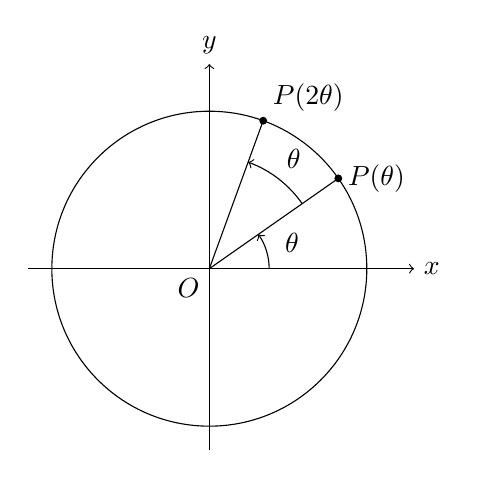
\begin{tikzpicture}[scale=2]
    \draw[->] (-1.15,0) -- (1.3,0) node[right] {$x$};
    \draw[->] (0,-1.15) -- (0,1.3) node[above] {$y$};
    \draw (0,0) circle (1);
    \node[below left] at (0,0) {$O$};
    \draw (0,0) -- (35:1);
    \draw (0,0) -- (70:1);
    \fill (35:1) circle (0.025) node[right] {$P(\theta)$};
    \fill (70:1) circle (0.025) node[above right] {$P(2\theta)$};
    \draw[->] (0.38,0) arc (0:35:0.38);
    \node at (17.5:0.55) {$\theta$};
    \draw[->] (35:0.72) arc (35:70:0.72);
    \node at (52.5:0.88) {$\theta$};
  \end{tikzpicture}
  \BookFigureCaption{単位円における角度の倍化}
\end{center}

先ほどの\bookterm{sequence}{数列}では,$a_n$は点$P(\theta_n)$の横座標である.
回転後の横座標が
\[
  \cos(2\theta_n)=2\cos^2\theta_n-1=2a_n^2-1
\]
となり,更新を満たす.初めの角度は
\[
  \frac{\pi}{6}\ \longrightarrow\ \frac{\pi}{3}
  \ \longrightarrow\ \frac{2\pi}{3}
  \ \longrightarrow\ \frac{4\pi}{3}
\]
と変わり,横座標は
\[
  \frac{\sqrt{3}}{2}\ \longrightarrow\ \frac12
  \ \longrightarrow\ -\frac12
  \ \longrightarrow\ -\frac12
\]
と変わる.最後の二点は異なるが横座標は同じであり,\bookterm{sequence}{数列}の値だけでは点の動きを捉えきれない.

一定角の回転なら$\theta_{n+1}=\theta_n+\phi$だが,倍角では回す角度が毎回変わる.
点の角度は$2\pi$ごとに読み替えてよい.$P(\theta)$と$P(\theta+\pi)$は倍角で同じ点へ移るため,円周全体の写像としても一定角の回転とは異なる.

\,\sectionref{節：複素平面と極形式}の見方を使えば,この操作はさらに短く書ける.
\[
  z_n=\cos\theta_n+i\sin\theta_n
\]
と置くと,\bookterm{de-moivre}{ド・モアブルの定理}より
\[
  z_{n+1}=z_n^2,\qquad z_n=z_1^{\,2^{n-1}}
\]
となる.絶対値1の$z_n$を自身に掛け,角度をもう一度加えた.$a_n$はその実部である.

\subsubsection{正接と傾き}\label{節：正接と傾き}
今度は
\[
  a_1=\tan\frac{\pi}{12}=2-\sqrt{3},
  \quad
  a_{n+1}=\frac{2a_n}{1-a_n^2}
\]
を考える.右辺は$\tan$の倍角公式そのものである.したがって,
\[
  a_n=\tan\left(2^{n-1}\frac{\pi}{12}\right)
\]
と予想できる.

初項に一致し,帰納法の段階では
\begin{align*}
  a_{n+1}
  &=\frac{2a_n}{1-a_n^2}\\
  &=\cfrac{2\tan\left(2^{n-1}\cfrac{\pi}{12}\right)}
  {1-\tan^2\left(2^{n-1}\cfrac{\pi}{12}\right)}\\
  &=\tan\left(2^n\frac{\pi}{12}\right)
\end{align*}
となる.分母が0にならないことは,角度から確かめる.

$a_n=\tan\theta_n$は,原点と$P(\theta_n)$を通る直線の傾きである.
倍角の動きを,今度は横座標でなく傾きで記録する.
直線の向きは$\pi$ごとに同じになるが,縦向きでは傾きが定義できない.
$a_n=\pm1$では$\cos(2\theta_n)=0$となり,この縦向きが分母$1-a_n^2=0$に対応する.
なお,この例の角度は,$n\geq2$では
\[
  \theta_n=\frac{2^{n-2}\pi}{6}
\]
である.$\displaystyle \theta_n=\frac{\pi}{2}+k\pi$となるには$2^{n-2}=3+6k$が必要だが,
2の累乗は3の倍数でないので不可能である.初項でも傾きは定義できるため,全項が定義される.

\subsubsection{角度の整数倍}\label{節：角度の整数倍}
両例の方針は,
\[
  a_n=\varphi(\theta_n),
  \quad
  \varphi(m\theta)=F_m(\varphi(\theta))
\]
を満たす関数と整数倍公式を探し,角度の更新を解くことである.

また,ここで現れた多項式
\[
  2x^2-1,
  \quad
  4x^3-3x
\]
も同じ族に属する.\bookterm{chebyshev}{チェビシェフ多項式}$T_m(x)$を
\[
  T_m(\cos\theta)=\cos(m\theta)
\]
で定義すれば,
\[
  T_0(x)=1,  T_1(x)=x,
\]
\[
  T_{m+1}(x)=2xT_m(x)-T_{m-1}(x)
\]
となる.例えば $T_2(x)=2x^2-1$ である.
$T$の添字は角度の倍率なので,$\cos$の例は
\[
  a_{n+1}=T_2(a_n),
  \quad
  a_n=T_{2^{n-1}}(a_1)
\]
と書ける.一回の更新では
\[
  T_2(T_m(\cos\theta))=T_{2m}(\cos\theta)
\]
となり,添字は$2,4,8,\ldots$と進む.
付録の\bookterm{chebyshev}{チェビシェフ多項式}では,この合成を一般の整数倍へ広げる.

\subsection{ニュートン法}\label{節：ニュートン法}

方程式の解へ近づく更新を,接線の傾き$f'(a)$から設計する.\footnote{微分が未習なら,接線と$x$軸の交点から次の近似値を作る図形的な発想と,得られた\bookterm{recurrence}{漸化式}の変形を先に読んでよい.}
曲線と$x$軸の交点を直接求める代わりに,今いる点の近くで曲線を接線に置き換える.
直線の交点なら一次方程式で求められる.その位置を次の近似値にし,同じ操作を繰り返す.
点$a$の近くでは,
\[
  f(a+h) \approx f(a)+f'(a)h
\]
と近似できる.方程式
\[
  f(x)=x^2-2=0
\]
の正の解を求めよう.正の近似値$a_n$での接線は,傾き$2a_n$より,
\[
  y=f(a_n)+2a_n(x-a_n)
\]
である.\,$y=0$ と置いて $x$ 軸との交点を求めると,
\begin{align*}
  a_{n+1}
  &=a_n-\frac{f(a_n)}{f'(a_n)}\\
  &=a_n-\frac{a_n^2-2}{2a_n}\\
  &=\frac{a_n^2+2}{2a_n}
\end{align*}
を得る.これが\bookterm{newton}{ニュートン法}の\bookterm{recurrence}{漸化式}である.
$a_1>0$から各項も正となり,分母は0にならない.
\BookFigNewton

例えば $a_1=2$ とすると,
\[
  a_2=\frac{3}{2},
  \quad
  a_3=\frac{17}{12},
  \quad
  a_4=\frac{577}{408}
\]
となり,これらは $\sqrt{2}$ に急速に近づく.この速さは,誤差を
$e_n=a_n-\sqrt{2}$ と置くと見える.
\begin{align*}
  e_{n+1}
  &=\frac{a_n^2+2}{2a_n}-\sqrt{2}\\
  &=\frac{(a_n-\sqrt{2})^2}{2a_n}\\
  &=\frac{e_n^2}{2a_n}
\end{align*}
誤差が小さくなると,分母は$2\sqrt2$に近づき,誤差は二乗に応じて減る.
\bookterm{general}{一般項}を求めるには,残る分母$a_n$を消したい.
$a_n-\sqrt2$と$a_n+\sqrt2$を並べると,
\BookMathLayout{
  \[
    \begin{aligned}
      a_{n+1}-\sqrt2&=\frac{(a_n-\sqrt2)^2}{2a_n},\\
      a_{n+1}+\sqrt2&=\frac{(a_n+\sqrt2)^2}{2a_n}
    \end{aligned}
  \]
}{
  \[
    \begin{aligned}
      a_{n+1}-\sqrt2&=\frac{(a_n-\sqrt2)^2}{2a_n},\\
      a_{n+1}+\sqrt2&=\frac{(a_n+\sqrt2)^2}{2a_n}
    \end{aligned}
  \]
}
となる.両辺の比を取ることで$2a_n$が消え,
\[
  \frac{a_{n+1}-\sqrt{2}}{a_{n+1}+\sqrt{2}}
  =\left(\frac{a_n-\sqrt{2}}{a_n+\sqrt{2}}\right)^{2}
\]
となる.そこで
\[
  b_n=\frac{a_n-\sqrt{2}}{a_n+\sqrt{2}}
\]
と置けば,$b_{n+1}=b_n^2$と\bookterm{logarithm}{対数}型(\sectionref{節：対数型})へ戻る.
\textbf{そのまま二乗されるのは誤差$e_n$ではなく,比$b_n$である.}

\,$a_1=2$のとき,\,$b_1=\dfrac{2-\sqrt2}{2+\sqrt2}=3-2\sqrt2=\dfrac1{3+2\sqrt2}$であるから,\,$u=3+2\sqrt2$とおくと$b_n=u^{-2^{n-1}}$である.これを$b_n=\dfrac{a_n-\sqrt2}{a_n+\sqrt2}$について$a_n$で解けば,
\[
  a_n=\sqrt{2}\,\frac{u^{2^{n-1}}+1}{u^{2^{n-1}}-1},\qquad u=3+2\sqrt2
\]
という閉じた式が得られる.
$u>1$なので,$u^{-2^{n-1}}$は$0$に近づき,$a_n$は$\sqrt2$に近づくことも分かる.

この閉じた式は$f(x)=x^2-2$に固有の変形から得たものである.
一般の\bookterm{newton}{ニュートン法}でも得られるとは限らないが,収束先や誤差は調べられる.
\sectionref*{節：和と差から微積分へ}では,更新の設計を収束,\bookterm{fixed}{不動点},誤差評価,微分方程式へ広げる.

\subsection{初項による違い}\label{節：初項による違い}

式の形に加えて,初項の選び方も解法を左右する.
\[
  a_1=c,
  \quad
  a_{n+1}=\frac{a_n^2-1}{2}
\]
初項を記号 $c$ のままにすると,
\begin{align*}
  a_2&=\frac{c^2-1}{2},\\
  a_3&=\frac{c^4-2c^2-3}{8},\\
  a_4&=\frac{c^8-4c^6-2c^4+12c^2-55}{128}
\end{align*}
一般に$a_n$は$c$の次数$2^{n-1}$の多項式となり,固定された簡単な表現が見えにくい.

特に $c=2$ と固定すると,
\[
  a_1=2,
  \quad
  a_2=\frac{3}{2},
  \quad
  a_3=\frac{5}{8},
  \quad
  a_4=-\frac{39}{128}
\]
となる.倍角や対称式の恒等式,接線近似はそのまま使えない.
図では$f(x)=\dfrac{x^2-1}{2}$とし,$a_1=2$から曲線$y=f(x)$へ縦に進み,直線$y=x$へ横に進む.
縦の移動で次の値を計算し,横の移動でそれを次の入力にする.
初項を変えれば,同じ更新でも別の軌道をたどる.
\BookFigCobweb

$c=2$で簡単な表現が見えなくても,他の初項まで同じとは限らない.
例えば,
\[
  c=1+\sqrt{2},
  \quad
  c=1-\sqrt{2}
\]
なら定数\bookterm{sequence}{数列}$a_n=c$となる.
一般の$c$では閉じた\bookterm{general}{一般項}が見つからなくても,
\[
  a_n=f^{\,\circ(n-1)}(c),
  \quad
  f(x)=\frac{x^2-1}{2}
\]
と書くことはできる.\footnote{$f^{\,\circ m}$は$f$を$m$回合成することを表し,$f^{\,\circ0}(c)=c$とする.関数の値の$m$乗とは異なる.}
これは更新の略記で,計算を済ませた式ではない.軌道,\bookterm{limit}{極限},近似を調べることもできる.
付録では\bookterm{matrix}{行列}や\bookterm{generating}{母関数}へ見方を広げる.

基本対称式型も,初項次第では直接分かる.
\[
  a_1=-1,\quad a_{n+1}=a_n^2-2
\]
なら$a_n=-1$となる.定数解は\bookterm{fixed}{不動点}の式
\[
  \alpha=\alpha^2-2
\]
の解$\alpha=-1,2$を初項に選べば得られる.

定数解$a_n=-1$も,\sectionref{節：対称式を使う}の$\alpha+\alpha^{-1}=a_1$による表示に含まれる.
その計算を複素数へ広げよう.\footnote{$\alpha^2-a_1\alpha+1=0$には複素数の範囲で必ず非零の解がある.$|a_1|<2$では$\alpha$が実数にならないため,実数の$\alpha$だけを使った先の例から一歩広げている.}
特に$-2\le a_1\le2$なら,$a_1=2\cos\theta$と書けるので,
$\alpha=e^{i\theta}$と選ぶと
\[
  a_n=\alpha^{2^{n-1}}+\alpha^{-2^{n-1}}=2\cos(2^{n-1}\theta)
\]
という\bookterm{trigonometric}{三角関数}の形になる.

$a_1=-1$では$\theta=\dfrac{2\pi}{3}$.倍角を$2\pi$ごとに読み替えると,$\dfrac{2\pi}{3}$と$\dfrac{4\pi}{3}$を行き来する.
どちらも余弦が$-\dfrac{1}{2}$なので$a_n=-1$となる.角度の動きを横座標に移すと,定数解になった.

\subsection{変わらない量を使う}\label{節：変わらない量を使う}
\sectionref*{節：対称式を使う}の恒等式に続き,\textbf{更新しても変わらない関係}を探す.
それを使い,\sectionref*{節：隣接3項型}へ帰着させる.

\subsubsection{例題：数項から候補を作る}
\[
  a_1=a_2=1,\qquad
  a_{n+2}=\frac{a_{n+1}^2+1}{a_n}\quad(n\ge1)
\]
を考える.初めの数項は$1,1,2,5,13,\ldots$である.
正の二項から次の項も正になるので,すべての分母は非零である.
$a_{n+2}=3a_{n+1}-a_n$と予想できるが,証明が要る.
$x=a_n,y=a_{n+1},z=a_{n+2}$とすれば$xz=y^2+1$で,$x,z$が対称に現れる.
$x+z=Ky$を目標にすると,係数の候補は
\[
  K=\frac{x+z}{y}=\frac{x^2+y^2+1}{xy}
\]
となる.\textbf{目標から,一定であってほしい量を作った.}

\bookstep{変わらないことを示す}
作った量を
\BookMathLayout{\[
    I_n=\frac{a_n^2+a_{n+1}^2+1}{a_na_{n+1}}
  \]}{\[
    \begin{aligned}
      I_n=\frac{a_n^2+a_{n+1}^2+1}{a_na_{n+1}}
    \end{aligned}
  \]}
とする.$xz=y^2+1$より,
\[
  \begin{aligned}
    \frac{x^2+y^2+1}{xy}&=\frac{x+z}{y},\\
    \frac{y^2+z^2+1}{yz}&=\frac{x+z}{y}
  \end{aligned}
\]
なので$I_{n+1}=I_n$である.
$I_1=3$だから,すべての$n$について
\[
  a_n+a_{n+2}=3a_{n+1}
\]
を得る.初めの二項を保ったまま\bookterm{linear}{線形}の\bookterm{recurrence}{漸化式}へ帰着できた.

\bookstep{一般項へ戻す}
$\alpha=\frac{3+\sqrt5}{2}$, $\beta=\frac{3-\sqrt5}{2}$とすると,
\bookterm{characteristic}{特性方程式}$x^2-3x+1=0$から
\[
  a_n=\frac{\alpha^{n-1}+\beta^{n-1}}2
  -\frac{\alpha^{n-1}-\beta^{n-1}}{2\sqrt5}
\]
を得る.初めの二項はともに1で,線形の更新の一意性から元の数列に一致する.
また,$a_{n+2}=3a_{n+1}-a_n$から整数性も帰納的に分かる.

\subsubsection{保存と線形化}
更新の前後で値が変わらない量を\textbf{\bookterm{invariant}{不変量}}という.
この例題では,保存される量から足し算と定数倍の\bookterm{linear}{線形}の関係を取り出した.\footnote{この\bookterm{linear}{線形}の式と元の式が全く同じ条件を表すと無条件に主張したわけではなく,
  元の数列について保存から導いた関係である.}

\begin{bookpoint}
  \textbf{\bookterm{invariant}{不変量}の使い方}\par
  初期値で保存量の値を決め,元の更新と合わせて解きやすい関係を取り出す.
  保存量の存在だけで\bookterm{general}{一般項}が求まるとは限らない.
\end{bookpoint}
初期値を変えたときの係数は\bookproblemref{practice-connections}{2}{接続演習問2},
整数方程式を保つ更新は\bookproblemref{practice-entrance}{9}{発展問9}へ.
付録の\sectionref*{節：演習を別の視点から}でも発展問9を扱う.

\subsection{非線形の周期性}\label{節：非線形の周期性}
\sectionref*{節：初項による違い}の定数解に続き,二項の組が戻ることで周期を示す.
\bookterm{general}{一般項}は先に求めなくてよい.

\bookstep{例：二項の組が戻る}
$a_{n+2}=\dfrac{1+a_{n+1}}{a_n}$で初めの二項をともに$1$にすると,
$1,1,2,3,2,1,1,\ldots$となる.
第6,7項が初めの二項に戻るので,その先も繰り返す.正の$x,y$へ広げよう.

\bookstep{一般の初期値で確かめる}
\[
  \begin{aligned}
    a_1&=x>0,\qquad a_2=y>0,\\
    a_{n+2}&=\frac{1+a_{n+1}}{a_n}\quad(n\ge1)
  \end{aligned}
\]
とする.正の二項から次も正になるため,すべての項が定義される.

\bookstep{最初の二項への復帰}
\BookMathLayout{\[
    a_3=\frac{1+y}{x},\qquad
    a_4=\frac{1+x+y}{xy},\qquad
    a_5=\frac{1+x}{y}
  \]}{\[
    \begin{aligned}
      a_3&=\frac{1+y}{x},\\
      a_4&=\frac{1+x+y}{xy},\\
      a_5&=\frac{1+x}{y}
    \end{aligned}
  \]}
となる.$a_5$では
\[
  a_5=\frac{xy+1+x+y}{y(1+y)}=\frac{1+x}{y}
\]
と因数分解した.さらに
\[
  a_6=\frac{1+a_5}{a_4}=x,\qquad
  a_7=\frac{1+a_6}{a_5}=y
\]
と二項の組が戻り,その先も同じ更新で決まる.従って,
\[
  a_{n+5}=a_n\qquad(n\ge1)
\]
である.

\bookstep{周期と最小周期}
定\bookterm{sequence}{数列}になる$x=y=\dfrac{1+\sqrt5}{2}$では最小周期は1,ほかは5である.
定数解の条件は$x=y=t>0$, $t^2=t+1$から得る.
最小周期は5の約数である.そうでなければ,5を最小周期で割った正の余りも周期となり,最小性に反する.

\begin{bookpoint}
  \textbf{周期を証明する条件}\par
  二項で更新が決まるなら,二項の組の復帰を示す.
  初項からの周期,途中からの周期,符号だけの振動は区別する.
\end{bookpoint}
\sectionref*{節：ガウス記号を含む式}の有限状態,\sectionref*{節：特性根が虚数の場合}の回転とは別の周期の仕組みである.
初項の例外は\bookproblemref{practice-connections}{5}{接続演習問5}で確かめよう.


  % section: 漸化式の分類

\section{解法の分類}\label{節：解法の分類}

解法の結論は,\bookterm{general}{一般項}の\bookterm{closed}{閉じた形},和や積の表示,周期・停止・整数性などの性質に分かれる.
和や積を簡単に計算できるかは別の問題であり,ガウス型のように値の意味を読むこともある.

\bookterm{closed}{閉じた形}の目安は,高校数学程度の関数を使い,演算の個数を$n$とともに増やさず表すことである.\footnote{多項式・有理関数・指数・対数・三角関数などを有限回の演算や合成で組み合わせたものを\bookterm{elementary}{初等関数}という.
  本書ではガウス記号や場合分けも使う.閉じた表示は,使ってよい関数の範囲を定めて考える.}
本書の方法で表せないことから,他の方法や関数でも表せないとは結論できない.

入口は「共通の更新へ帰着する」と「式の構造を使う」である.
前者を4つの基本パターンから応用パターン・発展的な解法へ広げ,後者では恒等式や初項を手掛かりにした.
ガウス型のように両者が重なることもある.
\BookFigClassification

分類は解法を探す案内であり,閉じた形まで求まる保証ではない.
それが見つからなくても\bookterm{sequence}{数列}は定義され,\bookterm{limit}{極限}や整数の性質は調べられる.
\bookproblemref{practice-entrance}{6}{発展問6}では,一般項を求めずに減り方を調べる.

\end{bookcolumns}
